\documentclass[11pt]{article}
\newcommand{\blind}{0}


\usepackage{setspace}
\doublespacing

\usepackage{amsmath}
\usepackage{graphicx}
\usepackage{multirow}
\usepackage{enumerate}
\usepackage[authoryear]{natbib}
\usepackage{url}
\usepackage[margin=1in]{geometry}


\usepackage{amsmath,amssymb,dsfont,color,bm,mathtools,enumitem}
\mathtoolsset{showonlyrefs}
\usepackage{amsthm}
\usepackage{subcaption}


\newtheorem{thm}{Theorem}
\newtheorem{lem}{Lemma}
\newtheorem{prop}{Proposition}
\newtheorem{pro}{Property}
\newtheorem{cor}{Corollary}

\theoremstyle{definition}
\newtheorem{defn}{Definition}
\newtheorem{assumption}{Assumption}
\newtheorem{example}{Example}
\newtheorem{rmk}{Remark}


\usepackage[parfill]{parskip}
\input macros.tex
\usepackage{mathrsfs}  
\def\caliB{\mathscr{B}}
%\usepackage{microtype}
\usepackage{wrapfig}
\newcommand*{\KeepStyleUnderBrace}[1]{%f
  \mathop{%
    \mathchoice
    {\underbrace{\displaystyle#1}}%
    {\underbrace{\textstyle#1}}%
    {\underbrace{\scriptstyle#1}}%
    {\underbrace{\scriptscriptstyle#1}}%
  }\limits
}
\usepackage{microtype}
\usepackage{wrapfig}

\allowdisplaybreaks
\usepackage[colorlinks,citecolor=blue]{hyperref}




%%%%%%%%%%%%%%%%%%%%%%%%%%%%%%%%%%%%%%%%%%%%%%%%%%%%%%%%%%%%%%%%%%%%%%%%%%%%%%





\begin{document}

\if1\blind
{ \title{Smooth Tensor Estimation with Unknown Permutations}
 \date{}
\author{%
Chanwoo Lee \\
University of Wisconsin -- Madison\\
\texttt{chanwoo.lee@wisc.edu} \\
\and
Miaoyan Wang \\
University of Wisconsin -- Madison\\
\texttt{miaoyan.wang@wisc.edu} \\
}

    \maketitle
} \fi

\if0\blind
{
 \date{}
  \title{Smooth Tensor Estimation with Unknown Permutations}
\author{}
\maketitle
} \fi

\vspace{-2cm}
\begin{abstract}%  
 We consider the problem of structured tensor denoising in the presence of unknown permutations. Such data problems arise commonly in recommendation system, neuroimaging, community detection, and multiway comparison applications. Here, we develop a general family of smooth tensor models up to arbitrary index permutations; the model incorporates the popular tensor block models and Lipschitz hypergraphon models as special cases. We show that a constrained least-squares estimator in the block-wise polynomial family achieves the minimax error bound. A phase transition phenomenon is revealed with respect to the smoothness threshold needed for optimal recovery. In particular, we find that a polynomial of degree up to {\footnotesize $(m-2)(m+1)/2$} is sufficient for accurate recovery of order-$m$ tensors, whereas higher degree exhibits no further benefits. This phenomenon reveals the intrinsic distinction for smooth tensor estimation problems with and without unknown permutations. Furthermore, we provide an efficient polynomial-time Borda count algorithm that provably achieves optimal rate under monotonicity assumptions. The efficacy of our procedure is demonstrated through both simulations and Chicago crime data analysis. 
  \end{abstract}


\noindent%
{\it Keywords:} Tensor estimation, latent permutation, diverging dimensionality, phase transition, statistical-computational efficiency. 


\clearpage
\section{Introduction}
\label{sec:intro}
Higher-order tensor datasets arise ubiquitously in modern data science applications, for instance, recommendation systems \citep{baltrunas2011incarmusic,bi2018multilayer}, social networks \citep{bickel2009nonparametric},
genomics \citep{hore2016tensor}, and neuroimaging \citep{zhou2013tensor}.
Tensor provides effective representation of data structure that classical vector- and matrix-based methods fail to capture. 
One example is music recommendation system~\citep{baltrunas2011incarmusic} that records ratings of songs from users on various contexts. This three-way tensor of user $\times$ song $\times$ context allows us to investigate interactions of users and songs in a context-specific manner.
Another example is network dataset that records the connections among a set of nodes. Pairwise interactions are often insufficient to capture the complex relationships, whereas multi-way interactions improve the understanding of networks in molecular system~\citep{young2018universality} and social sciences~\citep{wang2019multiway,han2020exact}. In both examples, higher-order tensors represent multi-way interactions in an efficient way.


Tensor estimation problem cannot be solved without imposing structures. An appropriate reordering of tensor entries often provides effective representation of the hidden salient structure. In the music recommendation example, suppose that we have certain criteria available (such as, similarities of music genres, ages of users, and importance of contexts) to reorder the songs, users, and contexts. Then, the sorted tensor will exhibit smooth structure, because entries from similar groups tend to have similar values. Similar observation applies to network examples. An $m$-uniform hypergraph network can be represented by an order-$m$ adjacency tensor, with entries indicating the presence and absence of $m$-way interactions among a set of nodes. Suppose the characteristics of individual nodes are available so that one can rearrange nodes based on their similarities. Then, the sorted adjacency tensor will exhibit smooth structure by the same reason.

\begin{figure}[t]
    \centering
    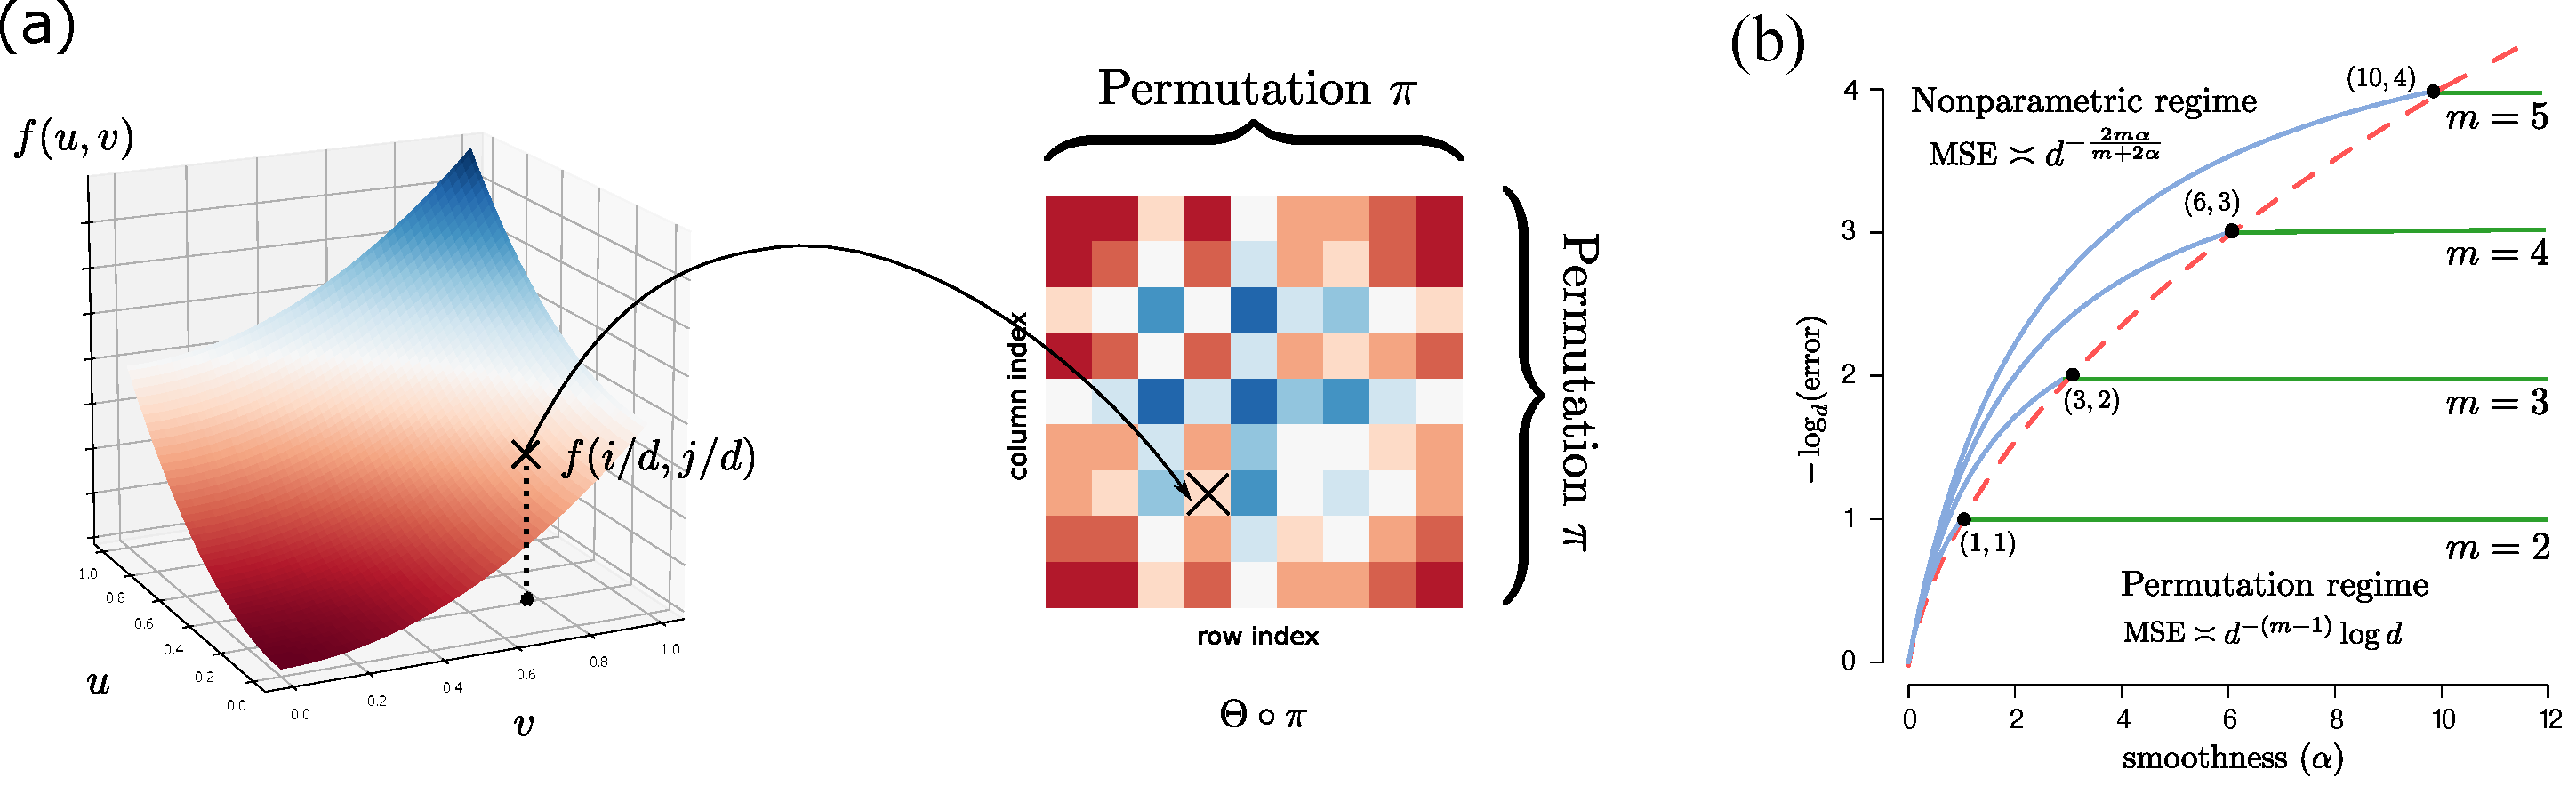
\includegraphics[width = .95\textwidth]{figure/semantic_new.pdf}
    \caption{(a): Illustration of order-$m$ $d$-dimensional permuted smooth tensor models with $m=2$. (b): Phase transition of mean squared error (MSE) (on $-\log_d$ scale) as a function of smoothness $\alpha$ and tensor order $m$. Bold dots correspond to the critical smoothness level above which higher smoothness exhibits no further benefits to tensor estimation. }
    \label{fig:rate}
\end{figure}


In this article, we develop a \emph{permuted} smooth tensor model based on the aforementioned  motivation. We study a class of structured tensors, called \emph{permuted smooth tensor model}, of the following form:
\begin{align}\label{eq:gmd}
    \tY = \Theta\circ \pi + \text{noise}, \quad \text{where}\quad \Theta(i_1,\ldots,i_m)=f\left({i_1\over d},\ldots,{i_m\over d}\right),
\end{align}
where $\pi\colon[d]\rightarrow[d]$ is an \emph{unknown} latent permutation, $\Theta$ is an \emph{unknown} order-$m$ $d$-dimensional signal tensor, and $f$ is an \emph{unknown} multivariate function with certain notion of smoothness, and $\Theta \circ \pi $ denotes the permuted tensor after reordering the indices along each of the $m$ modes. Figure~\ref{fig:rate}(a) shows an example of this generative model for the matrix case $m=2$. Our primary goal is to estimate the permuted smooth signal tensor $\Theta \circ \pi$ from the noisy tensor observation $\tY$ of arbitrary order $m$. 


\subsection{Our contributions}
We develop a suite of statistical theory, efficient algorithms, and related applications for permuted smooth tensor models~\eqref{eq:gmd}.  
Our contributions are summarized below. 

First, we develop a general permuted $\alpha$-smooth tensor model of arbitrary smoothness level $\alpha\geq 0$. We establish the statistically optimal error rate and its dependence on model complexity, including tensor order, tensor dimension, smoothness level, signal-to-noise ratio, and unknown permutations. Table~\ref{tab:comp} summarizes the comparison of our work with previous results.  Our framework substantially generalizes earlier works which focus on only matrices with $m=2$~\citep{gao2015rate,klopp2017oracle} or Lipschitz function with $\alpha=1$~\citep{balasubramanian2021nonparametric,li2019nearest}. The generalization enables us to obtain results previously impossible: i) As tensor order $m$ increases, we demonstrate the failure of pervious clustering-based algorithms~\citep{balasubramanian2021nonparametric,gao2015rate}, and we develop a new block-wise polynomial algorithm for tensors of order $m\geq 3$; ii) As smoothness $\alpha$ increases, we demonstrate that the error rate converges to a fast rate $\tO(d^{-(m-1)})$, thereby disproving the conjectured lower bound $\tO(d^{-2m/(m+2)})$ posed by earlier work~\citep{balasubramanian2021nonparametric}. The results showcase the accuracy gain of our new approach, as well as the intrinsic distinction between matrices and higher-order tensors. 

 \begin{table*}[t!]
    \centering
    \resizebox{\textwidth}{!}{%
    \begin{tabular}{c|@{\hskip4pt}c@{\hskip5pt}c@{\hskip4pt}c@{\hskip5pt}c@{\hskip4pt}c@{\hskip5pt}c@{\hskip4pt}c@{\hskip5pt}c}
    & \cite{pananjady2020isotonic}&  \citet{balasubramanian2021nonparametric}&  \citet{li2019nearest}&\textbf{Ours}\\
    \hline
       Model structure& monotonic & Lipschitz & Lipschitz &  $\alpha$-smoothness  \\
     Error rate for order-$m$ tensor$^*$ & \multirow{2}{*}{$d^{-1}$} & $d^{-{2m/(m+2)}}$ & $d^{-\lfloor m/3\rfloor }$ & $d^{-(m-1)}$ \\
       (e.g., when $m=3$) & & ($d^{-6/5}$) & $(d^{-1})$ & $(d^{-2})$ \\
          Minimax optimality& $\surd$  & $\times$ & $\times$ & $\surd$ \\
     Polynomial algorithm& $\surd$ &$\times$ & $\surd$ & $\surd$\\
    \end{tabular}
    }
    \caption{Comparison of our results with previous work. $^*$For simplicity, we list here the error rate (omitting the log term) for $\infty$-smooth tensors. Our results allow general tensors of arbitrary smoothness level $\alpha\geq 0$; See Theorems~\ref{thm:LSE}-\ref{thm:BC} in Sections~\ref{sec:lse}-\ref{sec:borda}.}\label{tab:comp}
\end{table*}

Second, we discover a phase transition phenomenon with respect to the smoothness needed for optimal recovery in model~\eqref{eq:gmd}. Figure~\ref{fig:rate}(b) plots the dependence of estimation error in terms of smoothness level $\alpha$ for tensors of order $m$. We characterize two distinct error behaviors determined by a critical smoothness threshold; see Theorems~\ref{thm:LSE}-\ref{thm:minimax} in Section~\ref{sec:lse}. Specifically, the accuracy improves with $\alpha$ in the regime $\alpha\leq m(m-1)/2$, but then it becomes a constant of $\alpha$ in the regime $\alpha>m(m-1)/2$. The results imply a polynomial of degree $(m-2)(m+1)/2$ $=[m(m-1)/2-1]$ is sufficient for accurate recovery of order-$m$ tensors of arbitrary smoothness in model~\eqref{eq:gmd}, whereas higher degree brings no further benefits. The phenomenon is distinctive from matrix problems~\citep{klopp2017oracle,gao2015rate} and classical \emph{non-permuted} smooth function estimation~\citep{tsybakov2009introduction}, thereby highlighting the fundamental challenges in our new setting. These statistical contributions, to our best knowledge, are new to the literature of general permuted smooth tensor problems. 

Third, we propose two estimation algorithms with accuracy guarantees: the least-squares estimation and Borda count estimation. The least-squares estimation, although being computationally hard, reveals the fundamental model complexity in the problem. The result serves as the benchmark and a useful guide to the algorithm design. Furthermore, we develop an efficient polynomial-time Borda count algorithm that provably achieves optimal rate under monotonicity assumptions. The algorithm handles a broad range of data types, including continuous and binary observations. 

Lastly, we illustrate the efficacy of our method through both simulations and data applications. A range of practical settings are investigated in simulations, and we show the outperformance of our method compared to alternative approaches.
Application to Chicago crime data is presented to showcase the usefulness of our method. We identify the key global pattern and pinpoint local smooth structure in the denoised tensor. Our method will help practitioners efficiently analyze tensor datasets in various areas. Toward this end, the package and all data used are released at CRAN.

\subsection{Related work}\label{sec:priorwork}
 Our work is closely related to but also clearly distinctive from several lines of existing research. We review related literature for comparison.
\paragraph{Structure learning with latent permutations.} The estimation problem of~\eqref{eq:gmd} falls into the general category of structured learning with \emph{latent permutation}. Models involving latent permutations have recently received a surge of interest, include graphons~\citep{chan2014consistent,klopp2017oracle}, stochastic transitivity models~\citep{chatterjee2015matrix,shah2019low}, statistical seriation~\citep{flammarion2019optimal,hutter2020estimation}, and graph matching~\citep{ding2021efficient,livi2013graph}. These methods, however, are developed for matrices; the tensor counterparts are far less well understood. Table~\ref{tab:comp} summarizes the most related works to ours. \citet{pananjady2020isotonic} studied the permuted tensor estimation under isotonic constraints.  We find that our smooth model results in a much faster rate $\tO(d^{-(m-1)})$ than the rate $\tO(d^{-1})$ for isotonic models. The works~\citep{balasubramanian2021nonparametric,li2019nearest} studied similar smooth models as ours, but we gain substantial improvement in both statistics and computations. \citet{balasubramanian2021nonparametric} developed a (non-polynomial-time) clustering-based algorithm with a rate $\tO(d^{-2m/(m+2)})$. \citet{li2019nearest} developed a (polynomial-time) nearest neighbor estimation with a rate $\tO(d^{-\lfloor m/3\rfloor})$. Neither approach investigates the minimax optimality. By contrast, we develop a polynomial-time algorithm with a fast rate $\tO(d^{-(m-1)})$ under mild conditions. The optimality of our estimator is safeguarded by matching a minimax lower bound. 


\paragraph{Low-rank tensor models.} There is a huge literature on structured tensor estimation under low-rank models, including CP models~\citep{kolda2009tensor,sun2017provable}, Tucker models~\citep{zhang2018tensor}, and block models~\citep{wang2019multiway}. These models belong to parametric approaches, because they aim to explain the data with a finite number of parameters (i.e., decomposed factors). Our permuted smooth tensor model utilizes a different measure of model complexity than the usual low-rankness. We use \emph{infinite} number of parameters (i.e., smooth functions) to allow growing model complexity. In this sense, our method belongs to nonparametric approaches. The comparison and benefits of nonparametric methods over parametric ones were discussed previously~\citep{pananjady2020isotonic,li2019nearest,gao2015rate,bickel2009nonparametric,shah2019low}.  
 
\paragraph{Nonparametric regression.} Our model is also related to nonparametric regression~\citep{tsybakov2009introduction}. One may view the problem~\eqref{eq:gmd} as a nonparametric regression, where the goal is to learn the function $f$ based on scalar response $\tY(i_1,\ldots,i_m)$ and design points $(\pi({i_1}),\ldots,\pi({i_m}))$ in $\bbR^m$; see Figure~\ref{fig:rate}(a). However, the \emph{unknown} permutation $\pi$ significantly influences the statistical and computational hardness of the problem. This latent $\pi$ leads to a phase transition behavior in the estimation error; see Figure~\ref{fig:rate}(b) and Sections~\ref{sec:lse}. We reveal  two components of error for the problem, one for nonparametric error and the other for permutation error. The impact of unknown permutation hinges on tensor order and smoothness in an intriguing way (see Theorems~\ref{thm:LSE}-\ref{thm:BC}). This is clearly contrary to classical nonparametric regression. 

\paragraph{Graphon and hypergraphon.} Our work is also connected to graphons and hypergraphons. Graphon is a measurable function representing the limit of a sequence of exchangeable random graphs (matrices)~\citep{klopp2017oracle,gao2015rate,chan2014consistent}. Similarly, hypergraphon~\citep{zhao2015hypergraph,lovasz2012large} is introduced as a limiting function of $m$-uniform hypergraphs, i.e., a generalization of graphs in which edges can join $m$ vertices with $m\geq 3$. While both our model~\eqref{eq:gmd} and hypergraphon focus on function representations, there are two remarkable differences. First, unlike the matrix case where graphon is represented as bivariate functions~\citep{lovasz2012large}, hypergraphons for $m$-uniform hypergraphs should be represented as $(2^m-2)$-multivariate functions; see~\citet[Section 1.2]{zhao2015hypergraph}. Our framework~\eqref{eq:gmd} represents the function using $m$ coordinates only, and in this sense, the model shares the common ground as \emph{simple hypergraphons}~\citep{balasubramanian2021nonparametric}. We compare our method to earlier work in theory (Table~\ref{tab:comp} and Sections~\ref{sec:lse}-\ref{sec:borda}) and in numerical studies (Section~\ref{sec:sim}). Second, unlike typical simple hypergraphons where the design points are random, our generative model uses deterministic design points. These two choices lead to different analysis in the same spirit as random- vs. fixed-designs in nonparametric regression~\citep{wasserman2006all,tsybakov2009introduction}. 

\subsection{Notation and organization}
We use $\bbN_{+}$ to denote the set of positive integers, and $\bbN_{\geq 0}=\bbN_{+}\cup\{0\}$.
We use $[d]=\{1,\ldots,d\}$ for $d$-set with $d\in\mathbb{N}_{+}$. For a set $S$, $|S|$ denotes its cardinality and $\mathds{1}_S$ denotes the indicator function. For two positive sequences $\{a_d\},\{b_d\}$,  we denote $a_d\lesssim b_d$ if $\lim_{d\to\infty} a_d/b_d\leq c$ for some constant $c>0$, and $a_d\asymp b_d$ if $c_1\leq \lim_{d\to \infty} a_d/b_d\leq c_2$ for some constants $c_1,c_2>0$. Given a number $a\in\bbR$, the floor function $\lfloor a\rfloor$ is the largest integer no greater than $a$, and the ceiling function $\lceil a\rceil$ is the smallest integer no less than $a$. We use $\tO(\cdot)$ to denote big-O notation hiding logarithmic factors, and $\circ$ the function composition. 

Let $\Theta\in\bbR^{d\times \cdots \times d}$ be an order-$m$ $d$-dimensional tensor, $\pi\colon[d]\rightarrow[d]$ be an index permutation, and $\Theta(i_1,\ldots,i_m)$ the tensor entry indexed by $(i_1,\ldots,i_m)$. We use $\Theta\circ\pi$ to denote the permuted tensor such that $(\Theta\circ\pi)(i_1,\ldots,i_m) = \Theta(\pi(i_1),\ldots,\pi(i_m))$ for all $(i_1,\ldots,i_m)\in[d]^m$. We sometimes  use shorthand notation $\Theta(\omega)$ for tensor entries with indices $\omega=(i_1,\ldots,i_w)$. We call a tensor \emph{a binary-valued tensor} if its entries take value on $\{0,1\}$-labels, and \emph{a continues-valued tensor} if its entries take values on a continuous scale. We define the Frobounis norm $\FnormSize{}{\Theta}^2=\sum_{\omega\in[d]^m}|\Theta(\omega)|^2$ for a tensor $\Theta$, and the $\infty$-norm $\mnorm{\mx}=\max_{i}|x_i|$ for a vector $\mx=(x_1,\ldots,x_d)^T$.
We use $\Pi(d,d)=\{\pi\colon [d]\to[d]\}$ to denote all permutations on $[d]$, while $\Pi(d,k)=\{\pi\colon [d]\to[k]\}$ the collection of all onto mappings from $[d]$ to $[k]$. An event $A$ is said to occur \emph{with high probability} if $\mathbb{P}(A)$ tends to 1 as the tensor dimension $d\to\infty$. 


The rest of the paper is organized as follows. Section~\ref{sec:model} presents the permuted smooth tensor model and its connection to smooth function representation. In Section~\ref{sec:tba}, we establish the approximation error based on block-wise polynomial approximation. In the next two sections,  we develop two estimation algorithms with accuracy guarantees: the least-squares estimation and Borda count estimation. Section~\ref{sec:lse} presents a statistically optimal but computationally challenging least-squares estimator. Section~\ref{sec:borda} presents a polynomial-time Borda count algorithm with a provably same optimal rate under monotonicity assumptions. Simulations and data analyses are presented in Section~\ref{sec:sim}.  We conclude the paper with a discussion in Section~\ref{sec:discussion}. Extra simulation results, proof for the main theorems, and technical lemmas are deferred to Appendix. 


\section{Smooth tensor model with unknown permutation}\label{sec:model}
Suppose we observe an order-$m$ $d$-dimensional data tensor from the following model,
\begin{equation}\label{eq:obs}
\tY=\Theta\circ \pi+\tE,
\end{equation}
where $\pi\colon[d]\rightarrow[d]$ is an unknown latent permutation,  $\Theta\in \bbR^{d\times \cdots \times d}$ is an unknown signal tensor under certain smoothness (to be specified in next paragraph), and $\tE$ is a noise tensor consisting of zero-mean, independent sub-Gaussian entries with variance bounded by $\sigma^2$. We allow heterogeneous and non-identically distributed entries in noise $\tE$. For instance, we allow binary tensor problem where entries in $\tY$ are $\{0, 1\}$-labels from Bernoulli distribution, in which case, the noise variance depends on the mean. Our model~\eqref{eq:obs} is applicable to a wide range of data types including continuous and binary tensors. 
 

We now describe the smooth model on the signal $\Theta$. Suppose that there exists a multivariate function $f\colon [0,1]^m\rightarrow \bbR$ underlying the signal tensor, such that
\begin{align}\label{eq:rep}
\Theta(i_1,\ldots,i_m) = f\left({i_1\over d},\ldots,{i_m\over d}\right), \quad \text{for all }(i_1,\ldots,i_m)\in[d]^m.
\end{align}
Assume the generative function $f$ is in the $\alpha$-H\"older smooth family~\citep{wasserman2006all,tsybakov2009introduction}. 
\begin{defn}[$\alpha$-H\"older smooth]
Let $\alpha\geq 0$. A function $f\colon [0,1]^m\rightarrow \bbR$ is $\alpha$-H\"older smooth, denoted as $f\in\tH(\alpha,L)$, if there exists a polynomial function $\textup{Poly}_{\lfloor \alpha\rfloor}(\mx-\mx_0)$ of degree  $\lfloor \alpha\rfloor$, such that 
\begin{align}\label{eq:defn}
    |f(\mx) - \textup{Poly}_{\lfloor \alpha\rfloor}(\mx-\mx_0)| \leq L\|\mx-\mx_0\|_\infty^\alpha,
\end{align}
for all $\mx,\mx_0\in [0,1]^m$ and a universal constant $L>0.$ 
\end{defn}
H\"older smooth function class is one of the most popular function classes considered in the nonparametric regression literature \citep{klopp2017oracle,gao2015rate}. 
In addition to the function class $\tH(\alpha, L)$, we also define the smooth tensor class based on discretization~\eqref{eq:rep}, 
\[
{\small \tP(\alpha,L)= \left\{\Theta\in\mathbb{R}^{d\times \cdots \times d} \colon\Theta(\omega) = f\left({\omega \over d}\right) \text{ for all } \omega=(i_1,\ldots,i_m) \in[d]^m \text{ and } f\in\tH(\alpha,L)\right\}.}
\]
Combining~\eqref{eq:obs} and~\eqref{eq:rep} yields our proposed \emph{permuted smooth tensor model}. 
The unknown parameters are the smooth tensor $\Theta \in \tP(\alpha, L)$ and latent permutation $\pi \in \Pi(d,d)$. The generative model is visualized in Figure~\ref{fig:rate}(a) for the case $m=2$ (matrices). For ease of presentation, we mainly consider the tensor model of equal dimension and same permutations along $m$ modes. The results for non-symmetric tensors with $m$ distinct permutations are similar but require extra notations; we assess this general case in Section~\ref{sec:sim}. 

We give two examples to show the applicability of our permuted smooth tensor model. 


\begin{example}[Four-player game tensors] Consider the tournament of a four-player board game. Suppose there are in total $d$ players, among which all combinations of four have played with each other. The tournament results are summarized as an order-4 (non-symmetric) tensor, with entries encoding the winner out of the four. Our model is then given by
\begin{align}
\bbE\tY(i_1,\ldots,i_4)&=\mathbb{P}(\text{player $i_1$ wins over $(i_2,i_3,i_4)$})\\&
=f\left({\pi(i_1)\over d},\cdots, {\pi(i_4)\over d}\right).
\end{align}
In this setting, we can interpret the permutation $\pi$ as the unknown ranking among $d$ players, and the function $f$ as the unknown four-player interaction. Players with similar ranking may have similar performance reflected by the smoothness of $f$. For example, a variant of popular Plackett-Luce model~\citep{chen2021optimal} considers the parametric form $f(x_1,x_2,x_3,x_4)={\exp(\beta x_1)/ \sum_{i=1}^4\exp(\beta x_i)}$. By contrast, our model leaves the form of $f$ unspecified, and we learn the function from the data in a nonparametric approach. 
\end{example}

\begin{example}[Co-authorship networks] Consider a co-authorship network consisting of $d$ nodes (authors) in total. We say there exists a hyperedge of size $m$ between nodes $(i_1,\ldots,i_m)$ if the authors $i_1,\ldots,i_m$ have co-authored at least one paper. The resulting $m$-uniform hypergraph is represented as an order-$m$ (symmetric) adjacency tensor. Our model is then expressed as
\begin{align}
    \bbE\tY(i_1,\ldots,i_m)&=\mathbb{P}(\text{authors $i_1,\ldots,i_m$ co-authored})\\&
=f\left({\pi(i_1)\over d},\cdots, {\pi(i_m)\over d}\right).
\end{align}
In this setting, we can interpret the permutation $\pi$ as the affinity measures of authors, and the function $f$ represents the $m$-way interaction among authors. The parametric model~\citep{wang2018learning} imposes logistic function $f(x_1,\ldots,x_m)=(1+\exp(-\beta x_1x_2\cdots x_m))^{-1}$. By contrast, our nonparametric model allows unknown $f$ and learns the function directly from data. 
\end{example}


\section{Block-wise tensor estimation}\label{sec:tba}
Our general strategy for estimating the permuted smooth tensor is based on the block-wise tensor approximation. In this section, we first introduce the tensor block model~\citep{wang2019multiway,han2020exact}. Then, we extend this model to block-wise polynomial approximation.

\subsection{Tensor block model}\label{subsec:bm}
Tensor block models describe a checkerboard pattern in a signal tensor. The block model provides a meta structure to many popular models including the low-rankness~\citep{young2018universality}, latent space models~\citep{wang2018learning}, and isotonic tensors~\citep{pananjady2020isotonic}. Here, we use tensor block models as a building block for estimating permutated smooth models. 

Specifically, suppose that there are $k$ clusters among $d$ entities, and the cluster assignment is represented by a clustering function $z \colon[d]\rightarrow[k]$. Then, the tensor block model assumes that the entries of signal tensor $\Theta\in\bbR^{d\times \cdots \times d}$ take values from a core tensor $\tS\in\bbR^{k\times\cdots\times k}$ according to the clustering function $z$; that is,
\begin{align}\label{eq:block}
    \Theta(i_1,\ldots,i_m) = \tS(z(i_1),\ldots,z(i_m)), \quad \text{ for all } (i_1,\ldots,i_m)\in[d]^m.
\end{align}
Here, the core tensor $\tS$ collects the entry values of $m$-way blocks; the core tensor $\tS$ and clustering function $z\in \Pi(d,k)$ are parameters of interest. A tensor $\Theta$ satisfying~\eqref{eq:block} is called a block-$k$ tensor, where $k$ is often assumed much smaller than $d$. Tensor block models allow various data types, as shown below. 

\begin{example}[Gaussian tensor block model] Let $\tY$ be a continuous-valued tensor. The Gaussian tensor block model draws independent entries according to $\tY(i_1,\ldots,i_m)\stackrel{\text{ind}}{\sim} N(\tS(z(i_1),\ldots,z(i_m)),\sigma^2)$. The mean model belongs to~\eqref{eq:block}, and the noise has subGaussian parameter $\sigma^2$. The Gaussian tensor block model has served as the statistical foundation for many tensor clustering algorithms \citep{wang2019multiway,han2020exact}.
\end{example}

\begin{example}[Stochastic tensor block model] Let $\tY$ be a binary-valued tensor. The stochastic tensor block model draws independent Bernoulli entries according to $\mathbb{P}(\tY(i_1,\ldots,i_m)=1)=\tS(z(i_1),\ldots,z(i_m))$. The mean model also belongs to \eqref{eq:block}, and the noise has subGaussianity parameter $\sigma$ bounded by $1/4$.  
The stochastic tensor block model is useful for community detection in multi-relational networks~\citep{bickel2009nonparametric,gao2015rate}.
\end{example}

Tensor block models have shown great success in discovering hidden group structures for many applications~\citep{wang2019multiway,han2020exact}. Despite the popularity, the constant block assumption is insufficient to capture delicate structure when the signal tensor is complicated. 
This parametric model aims to explain data with a finite number of blocks; such an approach is useful when the sample outsizes the parameters. Our nonparametric model~\eqref{eq:rep}, by contrast, uses infinite number of parameters (i.e., smooth functions) to allow growing model complexity. Our next section will shift the goal of tensor block model from discovering hidden group structures to approximating the generative function $f$ in~\eqref{eq:rep}. In our setting, the number of blocks $k$ should be interpreted as a resolution parameter (i.e., a bandwidth) of the approximation, similar to the notion of number of bins in histogram and polynomial regression~\citep{wasserman2006all}. 

\subsection{Block-wise polynomial approximation}\label{sec:poly}
The block tensor~\eqref{eq:block} can be viewed as a discrete version of piece-wise \emph{constant} function with $\alpha=0$ in~\eqref{eq:defn}. This connection motivates us to use block-wise \emph{polynomial} tensors to approximate $\alpha$-H\"older functions. Now we extend~\eqref{eq:block} to block-wise polynomial models. 

We introduce some additional notations. For a given block number $k$, we use $z\in\Pi(d,k)$ to denote the canonical clustering function that partitions $[d]$ into $k$ equally-sized clusters such that 
$z(i) = \lceil ki/d\rceil$, for all $i\in[d]$.
The collection of inverse images $\{z^{-1}(j)\colon j\in[k]\}$ is a partition of $[d]$ into $k$ disjoint and equal-sized subsets. We use $\tE_k$ to denote the $m$-way partition, i.e., a collection of $k^m$ disjoint and equal-sized subsets in $[d]^m$, such that 
\begin{align}\label{eq:blockind}
    \tE_k = \{z^{-1}(j_1)\times\cdots\times z^{-1}(j_m)\colon (j_1,\ldots,j_m)\in [k]^m\}.
\end{align}
Let $\Delta\in \tE_k$ denote the element in $\tE_k$. We propose to approximate the signal tensor $\Theta$ in~\eqref{eq:rep} by degree-$\ell$ polynomial tensors within each block $\Delta\in \tE_k$. Specifically, let $\caliB(k,\ell)$ denote the class of block-$k$ degree-$\ell$ polynomial tensors,
\begin{align}\label{eq:polynomial}
    \caliB(k,\ell) = \bigg\{&\tB\in \bbR^{d\times \cdots \times d}\colon \tB(\omega) = \sum_{\Delta\in\tE_k}\text{Poly}_{\ell,\Delta}(\omega)\mathds{1}\{\omega\in\Delta\}\text{ for all } \omega\in[d]^m\bigg\},
\end{align}
where $\text{Poly}_{\ell,\Delta}(\cdot)$ denotes a degree-$\ell$ polynomial function in $\bbR^m$, with coefficients depending on block $\Delta$; that is, a constant function $\text{Poly}_{0,\Delta}(\omega)= \beta^0_{\Delta}$ for $\ell=0$, a linear function $\text{Poly}_{1,\Delta}(\omega)=\langle \boldsymbol{\beta}_{\Delta},\omega\rangle+\beta_{\Delta}^0$ for $\ell=1$, and so on so forth. Here $\beta^0_{\Delta}$ and $\boldsymbol{\beta}_{\Delta}$ denote unknown coefficients in polynomial function. Note that the degree-0 polynomial block tensor reduces to the constant block model~\eqref{eq:block}. We generalize the constant block model to degree-$\ell$ polynomial block tensor~\eqref{eq:polynomial}, in a way that is analogous to the generalization from $k$-bin histogram to $k$-piece-wise polynomial regression in nonparametric statistics~\citep{wasserman2006all}.

Smoothness of the function $f$ in \eqref{eq:rep} plays an important role in the block-wise polynomial approximation. The following lemma explains the role of smoothness in the approximation. 

\begin{lem}[Block-wise polynomial tensor approximation]\label{lem:approx}
Suppose  $\Theta\in\tP(\alpha,L)$. Then, for every block number $k\leq d$, and degree $\ell\in \bbN_{\geq 0}$, we have the approximation error
\begin{align}
   \inf_{\tB\in\caliB(k,\ell)} \frac{1}{d^m}\FnormSize{}{\Theta-\tB}^2\lesssim \frac{L^2}{k^{2\min(\alpha,\ell+1)}}.
\end{align}
\end{lem}
Lemma~\ref{lem:approx} implies that we can always find a block-wise polynomial tensor close to the signal tensor generated from $\alpha$-H\"older smooth function $f$. The approximation error decays with block number $k$ and degree $\min(\alpha,\ell+1)$. 

\section{Fundamental limits via least-squares estimation}\label{sec:lse}
We develop two estimation methods based on the block-wise polynomial approximation. We first introduce a statistically optimal but computationally inefficient least-squares estimator. The least-squares estimation serves as a statistical benchmark because of its minimax optimality. In Section~\ref{sec:borda}, we will present a polynomial-time algorithm with a provably same optimal rate under monotonicity assumptions.

We propose the least-squares estimation for model~\eqref{eq:obs} by minimizing the Frobounis loss over the block-$k$ degree-$\ell$ polynomial tensor family $\caliB(k,\ell)$ up to permutations, 
\begin{align}\label{eq:lseopt}
    (\hat\Theta^{\text{LSE}},\hat \pi^{\text{LSE}}) &= \argmin_{\Theta\in\caliB(k,\ell), \pi\in \Pi(d,d)}\FnormSize{}{\tY-\Theta\circ\pi}.
\end{align}
The least-squares estimator $(\hat\Theta^{\text{LSE}},\hat\pi^{\text{LSE}})$ depends on two tuning parameters: the number of blocks $k$ and the polynomial degree $\ell$. The optimal choice $(k^*,\ell^*)$ will be provided below. 

Our next Theorem~\ref{thm:LSE} establishes the error bound for the least-squares estimator~\eqref{eq:lseopt}. Note that $\Theta$ and $\pi$ are in general not separably identifiable; for example, when the true signal is a constant tensor, then every permutation $\pi\in \Pi(d,d)$ gives equally good fit in statistics. We assess the estimation error on the composition $\Theta \circ \pi$ to avoid this identifiability issue. For two order-$m$ $d$-dimensional tensors $\Theta_1, \Theta_2$, define the mean squared error (MSE) by $\textup{MSE}(\Theta_1,\Theta_2) = d^{-m}\FnormSize{}{\Theta_1-\Theta_2}^2$. 
 
\begin{thm}[Least-squares estimation error]\label{thm:LSE} Consider the order-$m$ ($m\geq 2$) permuted smooth tensor model~\eqref{eq:obs} with $\Theta\in\tP(\alpha,L)$.
Let $(\hat\Theta^{\textup{LSE}},\hat\pi^{\textup{LSE}})$ denote the least-squares estimator in \eqref{eq:lseopt} with a given $(k,\ell)$. Then, for every $k\leq d$ and degree $\ell\in \mathbb{N}_{\geq 0}$, we have
\begin{align}\label{eq:rateMSE}
\textup{MSE}(\hat\Theta^{\textup{LSE}}\circ\hat\pi^{\textup{LSE}},\ \Theta\circ\pi)\lesssim \KeepStyleUnderBrace{\frac{L^2}{k^{2\min(\alpha,\ell+1)}}}_{\textup{approximation error}}+ \sigma^2\left(\KeepStyleUnderBrace{\frac{k^m(\ell+m)^\ell}{d^m}}_{\textup{nonparametric error}}+\KeepStyleUnderBrace{\frac{\log d}{d^{m-1}}}_{\textup{permutation error}}\right),
\end{align}
with high probability. In particular, setting {\small $\ell^* = \min(\lfloor \alpha\rfloor,(m-2)(m+1)/2)$} and $k^*=c_1 d^{m/(m+2\min(\alpha,\ell^*+1))}$
yields the optimized error rate
\begin{align}\label{eq:rates}
     \eqref{eq:rateMSE}\ \lesssim 
     \begin{cases} 
    c_2 d^{-\frac{2m\alpha}{m+2\alpha}}, & \text{ when } \alpha < m(m-1)/2,\\
     c_3 d^{-(m-1)}\log d, &\text{ when } \alpha \geq m(m-1)/2.
    \end{cases}
\end{align}
Here, the constants $c_1,c_2,c_3>0$ depend on the model configuration $(m,\sigma, L,\alpha)$ but not on the tensor dimension $d$. The closed-form expressions are provided in Section~\ref{sec:proofLSE}.
\end{thm}

We discuss the asymptotic error rate as $d\rightarrow \infty$ while treating other model configurations fixed. The final least-squares estimation rate~\eqref{eq:rates} has two sources of error: the nonparametric error $d^{-{2m\alpha\over m+2\alpha}}$ and the permutation error $d^{-(m-1)}\log d$. Intuitively, in the tensor data analysis problem, we can view each tensor entry as a data point, so sample size is the total number of entries, $d^m$. The unknown permutation results in $\log(d!)\approx d\log d$ complexity, whereas the unknown generative function results in $d^{-2m\alpha/(m+2\alpha)}$ nonparametric complexity. When the function $f$ is smooth enough, estimating the function $f$ becomes relatively easier compared to estimating the permutation $\pi$. This intuition coincides with the fact that the permutation error dominates the nonparametric error when  $\alpha\geq m(m-1)/2$. 


We now compare our results with existing work in the literature.
\begin{rmk}[Comparison to non-parametric regression]
In the vector case with $m = 1$,  our model reduces to the one-dimensional regression problem such that
\begin{align}
    y_i  = \theta_{\pi(i)}+\epsilon_i,  \quad\text{ for all } i\in [d],
\end{align}
where $\theta_i=f(i/d)$ and unknown $\pi \in \Pi(d,d)$.
A similar analysis of our Theorem~\ref{thm:LSE} shows the error rate
\begin{align}\label{eq:m1}
    \frac{1}{d}\sum_{i\in[d]}(\hat\theta_i^{\text{LSE}}-\theta_i)^2 \lesssim \left(d^{-{2\alpha\over 2\alpha+1}}+\log d\right),
\end{align}
under the choice of $\ell^* = 0$ and $k^* \asymp d^{1\over 1+2\min(\alpha,1)}$.
Notice that  $d^{-2\alpha/(2\alpha+1)}$ is the  classical nonparametric minimax rate for $\alpha$-Hölder smooth functions~\citep{tsybakov2009introduction} with \emph{known} permuted design points $\{\pi(i)\}_{i=1}^d$. By contrast, our model involves \emph{unknown} $\pi$, which results in the non-vanishing permutation rate $\log d$ in~\eqref{eq:m1}.
\end{rmk}

\begin{rmk}[Breaking previous limits on matrices/tensors]
In the matrix case with $m=2$, Theorem~\ref{thm:LSE} implies that the best rate is obtained under $\ell^*=0$, i.e., the block-wise \emph{constant} approximation. This result is consistent with existing literature on smooth graphons~\citep{bickel2009nonparametric,gao2015rate,klopp2017oracle}, where constant block model (see Section~\ref{subsec:bm}) has been develop for accurate estimation.

Earlier work~\citep{balasubramanian2021nonparametric} suggests that constant block approximation ($\ell^*=0$) remains minimax optimal for tensors of order $m\geq 3$. Our Theorem~\ref{thm:LSE} disproves this conjecture, and we reveal a much faster rate $d^{-(m-1)}$ compared to the conjectured lower bound $d^{-2m/( m+2)}$~\citep{balasubramanian2021nonparametric} for sufficiently smooth tensors. We demonstrate that a polynomial up to degree $(m-2)(m+1)/2$ is sufficient (and necessary; see Theorem~\ref{thm:minimax} below) for accurate estimation of order-$m$ permuted smooth tensors. 
In fact, permuted $\alpha$-smooth tensors of order-3 require quadratic approximation $(\ell^*=2)$ with $k^*\asymp d^{1/3}$ blocks, for all $\alpha\geq 2$. The results show the clear difference from matrices and highlight the challenges with tensors.
\end{rmk}


We now show that the rate in~\eqref{eq:rates} cannot be improved. The lower bound is obtained via information-theoretical analysis and thus applies to all estimators including, but not limited to, the least-squares estimator~\eqref{eq:lseopt} and Borda count estimator introduced in next section. 
\begin{thm}[Minimax lower bound]\label{thm:minimax}For any given $\alpha\geq 0$, the estimation problem based on model~\eqref{eq:gmd} obeys the minimax lower bound 
\begin{equation}\label{eq:minimax}
\inf_{(\hat \Theta,\hat \pi)}\sup_{
\Theta\in \tP(\alpha,L), \pi\in \Pi(d,d)} \mathbb{P}\left(\textup{MSE}(\hat\Theta\circ\hat\pi,\ \Theta\circ\pi) \gtrsim c_2 d^{-{2m\alpha\over m+2\alpha}}+c_3 d^{-(m-1)}\log d \right) \geq 0.8,
\end{equation}
where $c_2,c_3>0$ are the same constants as in Theorem~\ref{thm:LSE}. 
\end{thm}
The lower bound in~\eqref{eq:minimax} matches the upper bound in~\eqref{eq:rates}, demonstrating the statistical optimality of  least-squares estimator \eqref{eq:lseopt}. The two-component error reveals the intrinsic model complexity: the permutation error $d^{-(m-1)}$ dominates nonparametric error $d^{-{2m\alpha/(m+2\alpha)}}$ for sufficiently smooth tensors. This is clearly contrary to classical nonparametric regression. 

\begin{rmk}[Phase transition]\label{rmk:phase} We conclude this section by presenting an interesting phase transition phenomenon.  Figure~\ref{fig:rate}(b) plots the convergence rate of estimation error based on Theorems~\ref{thm:LSE}-\ref{thm:minimax}. We find that the impact of unknown permutation hinges on the tensor order and smoothness.  
The accuracy improves with smoothness in the regime $\alpha\leq m(m-1)/2$, but then it becomes a constant of smoothness in the regime $\alpha>m(m-1)/2$. 
The result implies a polynomial of degree $\approx (m-2)(m+1)/2$ is sufficient for accurate recovery of order-$m$ tensors, whereas higher degree brings no further benefits. This full picture of error dependence, to our best knowledge, is new to the literature of permuted smooth tensors.
\end{rmk}


\section{An efficient and computationally feasible procedure}\label{sec:borda}
At this point, we should point out that computing the least-squares optimizer $(\hat\Theta^{\text{LSE}},\hat\pi^{\text{LSE}})$ in \eqref{eq:lseopt} is generally computationally hard, even in the simple matrix case~\citep{gao2015rate}. In this section, we propose an efficient polynomial-time \emph{Borda count} algorithm. We show that Borda count estimator provably achieves the same convergence rate as the minimax lower bound~\eqref{eq:minimax} under monotonicity assumptions. 


\subsection{Borda count algorithm}
We introduce a notion of $\beta$-monotonicity for the generative functions.
\begin{defn}[Weakly $\beta$-monotonicity]\label{eq:bdefn}A function $f\colon[0,1]^m \rightarrow \bbR$ is called $\beta$-monotonic ($\beta\geq 0$), denoted as $f\in\tM(\beta)$, if there exists a small tolerance $\delta\lesssim d^{-(m-1)/2}$ such that
\begin{align}\label{eq:monotonic}
   \left({i-j\over d}\right)^{1/\beta}  \lesssim g(i)-g(j)+\delta,\quad \text{ for all } j<i\in[d],
\end{align}
where we define \emph{score function} $g(i) = d^{-(m-1)}\sum_{(i_2,\ldots,i_m)\in[d]^{m-1}} f\left({i\over d},{i_2\over d},\ldots,{i_m\over d}\right)$ for all $i \in[d]$.
\end{defn}

 
Our $\beta$-monotonicity condition extends the strictly monotonic degree condition in the graphon literature~\citep{chan2014consistent}; the latter is a special case of our definition with $\beta=1, m=2$ and $\delta=0$. A large value of $\beta$ in~\eqref{eq:monotonic} implies the steepness of $g$. The introduction of tolerance $\delta$ relaxes the condition by allowing for small fluctuations. Our $\beta$-monotonicity condition is also related to isotonic functions~\citep{pananjady2020isotonic} which consider more restricted coordinate-wise monotonicity; i.e., $f(x_1,\ldots,x_d)\leq f(x_1',\ldots,x_d')$
whenever $x_i\leq x_i'$ for $i\in[d]$. 

The $\beta$-monotonicity condition allows us to efficiently estimate the permutation $\pi$. Before presenting the theoretical guarantees, we provide the intuition here. The exponent $\beta$ measures the difficulty for estimating the permutation $\pi$. Consider the noisy observation $\tY$ from model \eqref{eq:gmd}.
We define the empirical score function $\tau\colon [d]\rightarrow\bbR$ as
\begin{align}\label{eq:score}
    \tau(i) = \frac{1}{d^{m-1}}\sum_{(i_2,\ldots,i_m)\in[d]^m} \tY(i,i_2,\ldots,i_m).
\end{align}
The permuted score function $\tau\circ\pi^{-1}$ reduces to the function $g$ in \eqref{eq:monotonic} under the noiseless setting.
Therefore, a good estimate $\hat\pi$ should make the permuted score function $\tau\circ\hat\pi^{-1}$ monotonically increasing. Notice that the estimated permutation $\hat\pi$ could be different from the oracle permutation $\pi$ due to the noise. We find that a larger $\beta$ guarantees a faster consistency rate of $\hat\pi$. A large $\beta$ implies large gaps of $|g(i)-g(j)|$ for $i\neq j$. Therefore, we obtain similar orderings of $\{\tau(i)\}_{i=1}^d$ before and after the addition of noise. This intuition is well represented by the following lemma.
\begin{lem}[Permutation error]\label{lem:permute}
Consider the permuted smooth tensor model with $f\in \tM(\beta)$. Let $\hat\pi$ be the permutation such that the permuted empirical score function $\tau\circ \hat\pi^{-1}$ is monotonically increasing. Then, with high probability, 
\begin{align}
    \textup{Loss}(\pi,\hat\pi):= \frac{1}{d}\max_{i\in[d]}|\pi(i)-\hat\pi(i)|\lesssim \left(\sigma d^{-(m-1)/2}\sqrt{\log d}\right)^{\beta}.
\end{align}
\end{lem}


Now we introduce the \emph{Borda count} estimation that consists of two stages. The full estimation procedure is illustrated in Figure~\ref{fig:borda}.
\begin{enumerate}[wide, labelwidth=0pt, labelindent=0pt]
  \item {\bf Sorting stage:} The purpose of the sorting is to rearrange the observed tensor $\tY$ so that the score function $\tau$ of sorted tensor is  monotonically increasing. We define a permutation $\hat\pi^{\text{BC}}$ such that
    \begin{align}\label{eq:permute}
        \tau((\hat\pi^{\text{BC}})^{-1}(1))\leq  \tau((\hat\pi^{\text{BC}})^{-1}(2))
        \leq \cdots 
        \leq
        \tau((\hat\pi^{\text{BC}})^{-1}(d)).
    \end{align}
    Then, we obtain sorted observation $\tilde\tY = \tY \circ (\hat\pi^{\text{BC}})^{-1}$, illustrated in Figure~\ref{fig:borda}(b).
\begin{figure}[t]
    \centering
    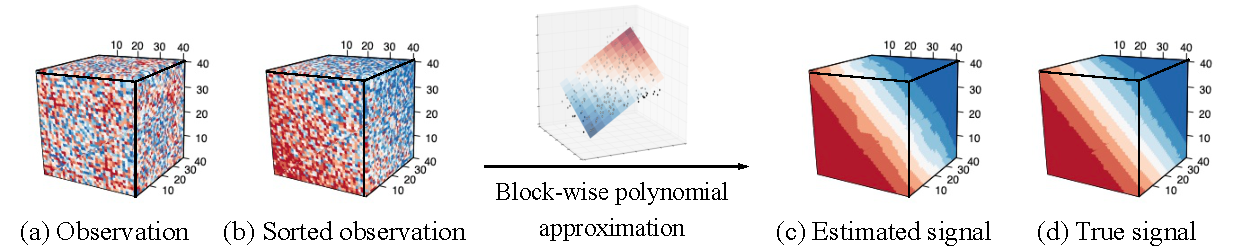
\includegraphics[width = \textwidth]{figure/Borda2.pdf}
    \caption{Illustration of Borda count estimation. We first sort tensor entries using the proposed procedure, and then estimate the signal by block-wise polynomial approximation.}
    \label{fig:borda}
\end{figure}

 \item {\bf Block-wise polynomial approximation stage:} Given sorted observation $\tilde \tY $, we estimate the signal tensor by block-wise polynomial tensor based on the following optimization,
    \begin{align}\label{eq:bclse}
        \hat\Theta^{\text{BC}} = \argmin_{\Theta\in\caliB(k,\ell)}\FnormSize{}{\tilde\tY-\Theta},
    \end{align}
    where $\tB(k,\ell)$ denotes the block-$k$ degree-$\ell$ tensor class  in~\eqref{eq:polynomial}. An example of this procedure is shown in Figure~\ref{fig:borda}(c).    
    \end{enumerate}
    
The pseudo algorithm is summarized below.
\begin{center}
\includegraphics[width=1\textwidth]{figure/algorithm_template.pdf}
\end{center}


The estimator $\hat\Theta^{\text{BC}}$ depends on two tuning parameters: the number of blocks $k$ and polynomial degree $\ell$. The optimal choice of $(k^*,\ell^*)$ is provided in Theorem~\ref{thm:BC}.
 Notice that the least-squares estimator in \eqref{eq:lseopt} requires a combinatoric search with exponential-time complexity for estimating the permutation. By contrast, the estimator~\eqref{eq:bclse} requires only the estimation of degree-$\ell$ polynomial within $k$ canonical blocks. Therefore, the Borda count estimator is polynomial-time efficient. Our algorithm implementation is available in CRAN. 



\subsection{Computational and statistical complexities}
In this section, we show that the Borda count estimation achieves both computational efficiency and statistical accuracy. 

The computational complexity of Borda count estimation is polynomial in tensor dimension $d$. In the sorting stage, computing the empirical score function $\tau$ requires $\tO(d^{m-1})$ operations while sorting the $\{\tau(i)\}_{i=1}^d$ requires $\tO(d\log d)$ comparisons. In the block-wise polynomial approximation stage, we compute $k^m$ many degree-$\ell$ polynomial tensors. Each polynomial tensor approximation requires $\tO((d/k)^m\ell)$ arithmetic operations. Thus, the second step requires $\tO(d^m\ell)$ operations. Combining the two steps yields the total complexity at most $\tO(d^m\log d)$. This complexity is comparable with existing efficient tensor estimation algorithms in other settings~\citep{li2019nearest,zhang2018tensor}.

The following theorem ensures the statistical accuracy of the Borda count estimator.
\begin{thm}[Estimation error for Borda count algorithm]\label{thm:BC} Consider the permuted smooth tensor model with $f\in \tH(\alpha,L)\cap \tM(\beta)$.
Let $(\hat\Theta^{\textup{BC}},\hat\pi^{\textup{BC}})$ be the Borda count estimator in \eqref{eq:permute}-\eqref{eq:bclse} with a given $(k,\ell)$. Then, for every $k\leq d$ and degree $\ell\in \mathbb{N}_{\geq 0}$, we have
\begin{align}\label{eq:BC}
     \textup{MSE}(\hat\Theta^{\textup{BC}}\circ\hat\pi^{\textup{BC}},\ \Theta\circ\pi)\lesssim  \frac{L^2}{k^{2\min(\alpha,\ell+1)}}+\sigma^2 \frac{k^m(\ell+m)^\ell}{d^m}+ \left(\sigma^2{\log d\over d^{m-1}}\right)^{\beta\min(\alpha,1)},
\end{align}
with high probability. Furthermore, denote a constant $c(\alpha,\beta,m):= \frac{m(m-1)\beta\min(\alpha,1)}{\max(0,\ 2(m-(m-1)\beta\min(\alpha,1)))}$. Then, setting {\footnotesize $
\ell^* = \min\left(\lfloor\alpha\rfloor,\lfloor c(\alpha,\beta,m)\rfloor\right)$} and $k^* = c_1d^{m/ (m+2\min(\alpha,\ell^*+1))}$ yields
\begin{align}\label{eq:rateBC}
  \eqref{eq:BC}\  \lesssim  
   \begin{cases}
   c_2 d^{-{2m\alpha\over m+2\alpha}} & \text{ when } \alpha <c(\alpha,\beta,m),\\
   \left({c_3\log d\over d^{m-1}}\right)^{\beta\min(\alpha,1)}&\text{ when } \alpha \geq c(\alpha,\beta,m),
   \end{cases}
\end{align}
where $c_1,c_2,c_3>0$ are the same constants as in Theorem~\ref{thm:LSE}.
\end{thm}


\begin{rmk}[Sufficiently smooth tensors] When the generative function is infinitely smooth ($\alpha =\infty$) with Lipschitz monotonic score $(\beta=1)$,
our estimation error~\eqref{eq:rateBC} becomes
\begin{equation}\label{eq:infinite}
\textup{MSE}(\hat\Theta^{\textup{BC}}\circ\hat\pi^{\textup{BC}},\ \Theta\circ\pi)\lesssim d^{-(m-1)}\log d,
\end{equation}
under the choice of degree and block number
\[
\ell^*= {(m-2)(m+1)/2}\quad \text{and}\quad k^* \asymp d^{m\over m +2\ell^*}.
\]
Now, we compare the rate~\eqref{eq:infinite} with the classical low-rank estimation~\citep{wang2018learning,zhang2018tensor,kolda2009tensor}. The low-rank tensor model with a constant rank is known to have MSE rate $\tO(d^{-(m-1)})$~\citep{wang2018learning}. Our infinitely smooth tensor model achieves the nearly same rate up to the negligible log term. Compared to low-rank models, we utilize a different measure of \emph{model complexity}.
When the underlying signal is precisely low-rank, then rank might be a reasonable measure for model complexity. However, if the underlying signal is high rank but has certain shape structure, then our nonparametric approach may better capture the intrinsic model complexity. 
\end{rmk}

\begin{rmk}[Comparison with least-squares estimation] The three terms in the estimation bound~\eqref{eq:BC} correspond to approximation error (Lemma~\ref{lem:approx}), nonparametric error (Theorem~\ref{thm:LSE}), and permutation error (Lemma~\ref{lem:permute}), respectively. 
We find that the Borda count estimator achieves the same minimax-optimal rate as the least-squares estimator for sufficiently smooth tensors under Lipschitz score condition $\beta =1$. The least-squares estimator requires a combinatoric search with exponential-time complexity. By contrast, the Borda count estimator is polynomial-time solvable. Therefore, Borda count algorithm enjoys both statistical accuracy and computational efficiency. 
\end{rmk}


\paragraph{Hyperparameter tuning.}
Our algorithm has two tuning parameters $(k,\ell)$. The theoretically optimal choices of $(k,\ell)$ are given in Theorems~\ref{thm:LSE} and~\ref{thm:BC}. In practice, since model configuration is unknown, we search $(k,\ell)$ via cross-validation. 
Based on our theorems, a polynomial of degree $\ell^*=(m-2)(m+1)/2$ is sufficient for accurate recovery of order-$m$ tensors, whereas higher degree brings no further benefit. The practical impacts of hyperparameter tuning are investigated in Section~\ref{sec:sim}. 

\section{Numerical analysis}\label{sec:sim}

\subsection{Synthetic data}
We simulate order-3 $d$-dimensional tensors based on the permuted smooth tensor model~\eqref{eq:rep}. Both symmetric and non-symmetric tensors are investigated. The symmetric tensors are generated based on functions $f$ in Table~\ref{tb:md}, and the non-symmetric results are discussed later.
\begin{table}[htp]
    \centering
    \begin{tabular}{c|c|c|c}
        Model ID  &  $f(x,y,z)$ & CP rank & Tucker rank \\\hline
        1 &    $xyz$ & 1 & $(1,1,1)$\\
        2 &    $(x+y+z)/3$ & 3 & $(2,2,2)$\\
        3 & $(1+\exp(-3x^2+3y^2+3z^2))^{-1}$ &9& $(4,4,4)$ \\
        4 & $\log(1+\max(x,y,z))$ &$\geq 100$& $\geq (50,50,50)$ \\
        5 &  $\exp\left(-\max(x,y,z)-\sqrt{x}-\sqrt{y}-\sqrt{z}\right)$ &$\geq 100$& $\geq (50,50,50$)
    \end{tabular}
    \caption{Smooth functions in simulation. We define the numerical CP/Tucker rank as the minimal rank $r$ for which the relative approximation error is below $10^{-4}$. The reported rank in the table is estimated from a $100\times100\times100$  signal tensor generated by \eqref{eq:rep}.}
    \label{tb:md}
\end{table}
The generative functions involve compositions of operations such as polynomial, logarithm, exponential, square roots, etc. Notice that considered functions cover a reasonable range of model complexities from low rank to high rank. Two types of noise are considered: Gaussian noise and Bernoulli noise.
For the Gaussian model, we simulate continuous-valued tensors with i.i.d.\ noises drawn from $N(0,0.5^2)$. For the Bernoulli model, we generate binary tensors $\tY$ using the success probability tensor $\Theta \circ \pi$. The permutation $\pi$ is randomly chosen. For space consideration, only results for Models 1, 3, and 5 are presented in the main paper. The rest is presented in Appendix~\ref{sec:extra}. We first examine impacts of model complexity to estimation accuracy. We then compare Borda count estimation with alternative methods under a range of scenarios. Extra simulation results and extensions are deferred to Appendix.


 \begin{figure}[t!]
    \centering
    \begin{subfigure}[b]{.9\textwidth}
    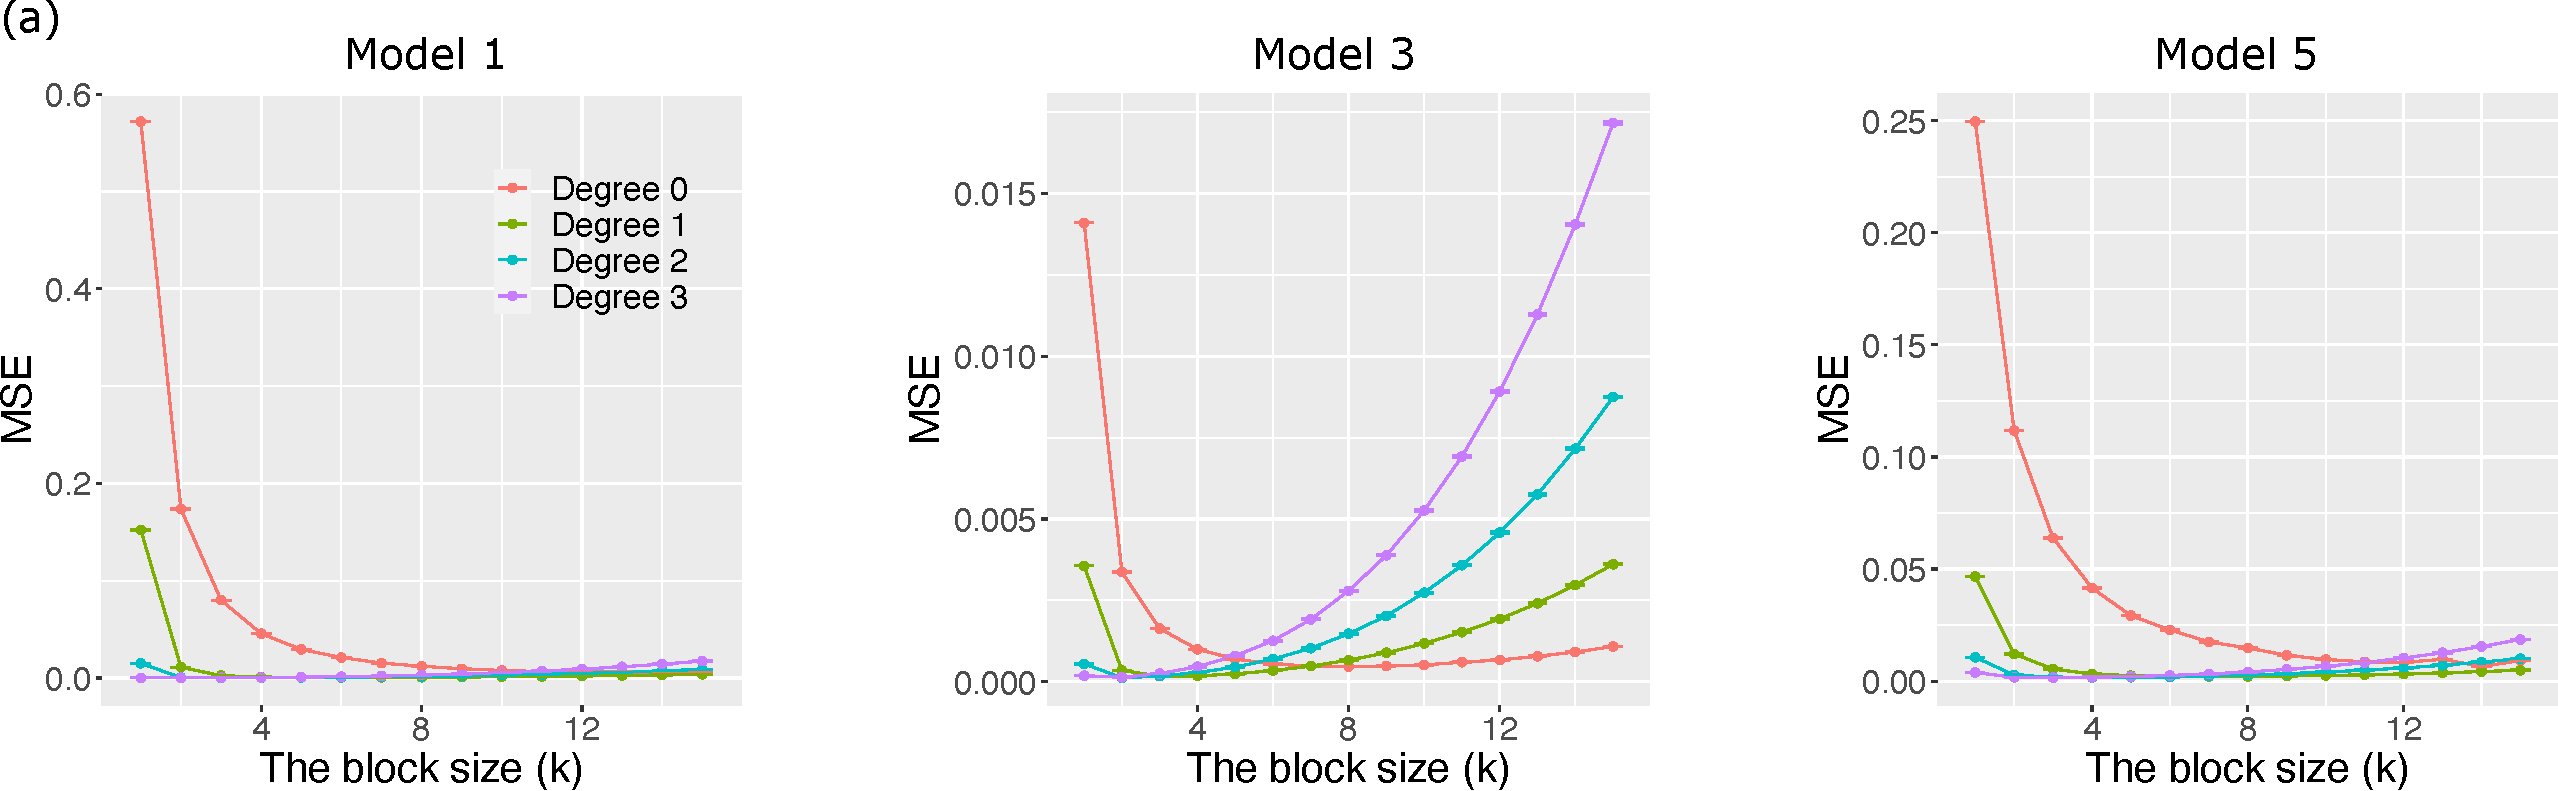
\includegraphics[width = \textwidth]{figure/deg_conti.pdf}    
    \end{subfigure}
    \vspace{.5cm}
    \begin{subfigure}[b]{.9\textwidth}
    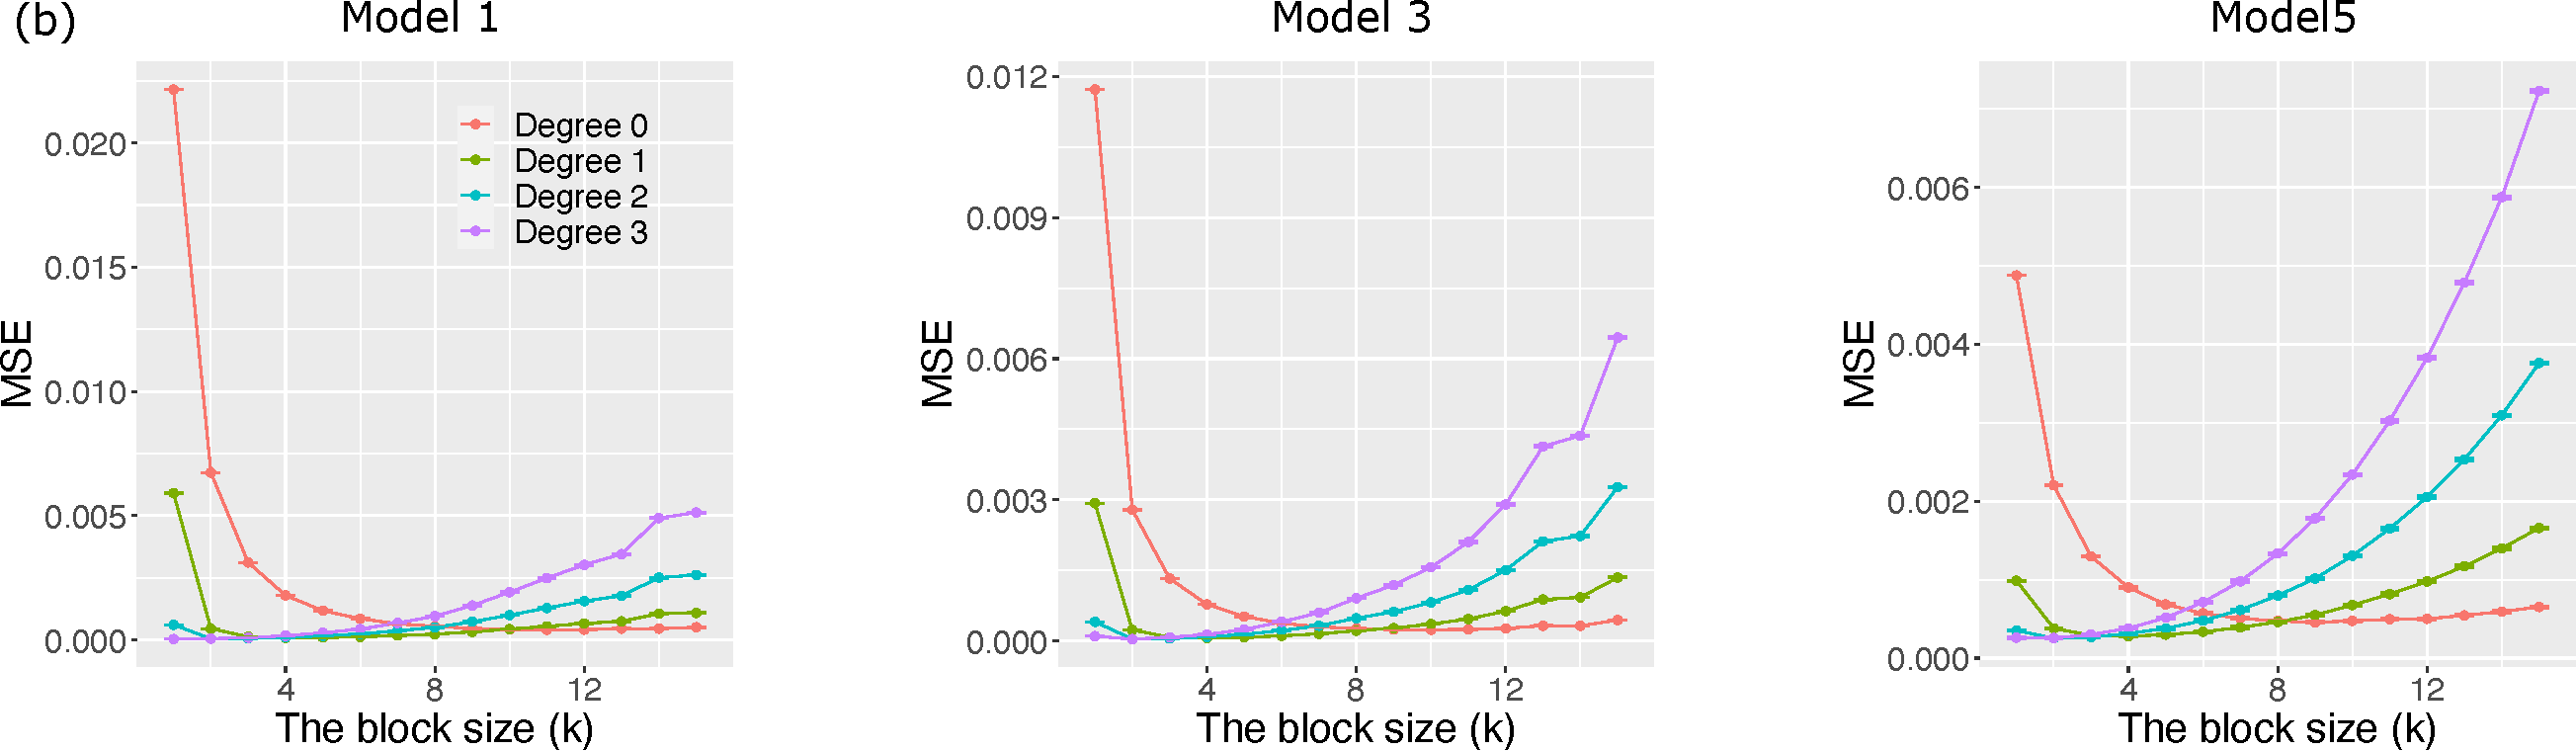
\includegraphics[width = \textwidth]{figure/deg_binary.pdf}    
    \end{subfigure}
    \caption{MSE versus the number of blocks based on different polynomial approximations. Columns 1-3 consider the Models 1, 3, and 5 respectively. Panel (a) is for continuous tensors, whereas (b) is for the binary tensors.}
    \label{fig:degk}
\end{figure}


\paragraph{Impacts of the number of blocks, tensor dimension, and polynomial degree.}
The first experiment examines the impact of the block number $k$ and degree of polynomial $\ell$ for the approximation. We fix the tensor dimension $d = 100$, and vary the number of blocks $k\in\{1,\ldots,15\}$ and polynomial degree $\ell\in\{0,1,2,3\}.$
Figure~\ref{fig:degk} demonstrates the trade-off in accuracy determined by the number of groups for each polynomial degree. The results confirm our bias-variance analysis in Theorem~\ref{thm:LSE}. While a large block number $k$ provides less biased approximation, this large $k$ renders the signal tensor estimation difficult within each block due to small sample size. In addition, we find that degree-2 polynomial approximation with the optimal $k$ gives the smallest MSE among all considered polynomial approximations. These observations are consistent with our theoretical results that the optimal number of blocks and polynomial degree are $(k^*,\ell^*)=(\tO(d^{3/7}),2)$. 



The second experiment investigates the impact of the tensor dimension $d$ for various polynomial degrees. We vary the tensor dimension $d\in\{10,\ldots,100\}$ and polynomial degree $\ell\in\{0,1,2,3\}$ in each model configuration. We set optimal number of blocks as the one that gives the best accuracy. Figure~\ref{fig:degdim} compares the estimation errors among different polynomial approximations. The result verifies that the degree-2 polynomial approximation performs the best under the sufficient tensor dimension, which is consistent with our theoretical results. We emphasize that this phenomenon is different from the matrix case where the degree-0 polynomial approximation gives the best results~\citep{gao2015rate,klopp2017oracle}.


\begin{figure}[ht!]
    \centering
    \begin{subfigure}[b]{.9\textwidth}
    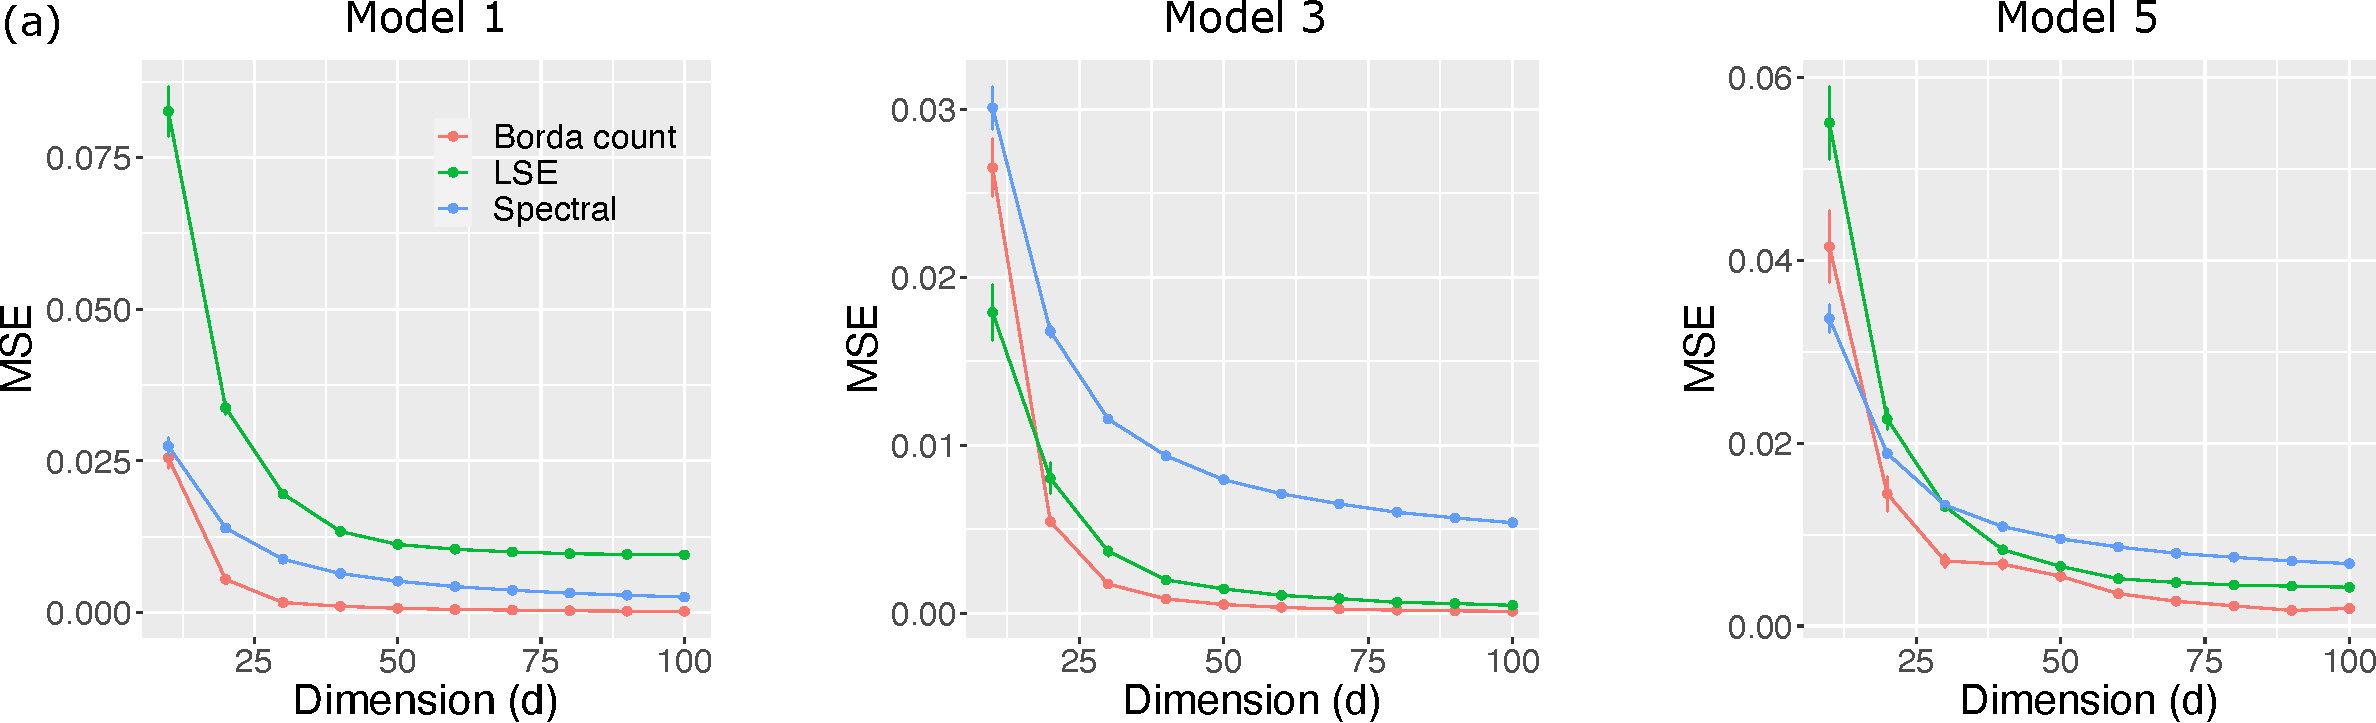
\includegraphics[width = \textwidth]{figure/altdim_conti.pdf}
       \vspace{.3cm}
    \end{subfigure}
    \begin{subfigure}[b]{.9\textwidth}
    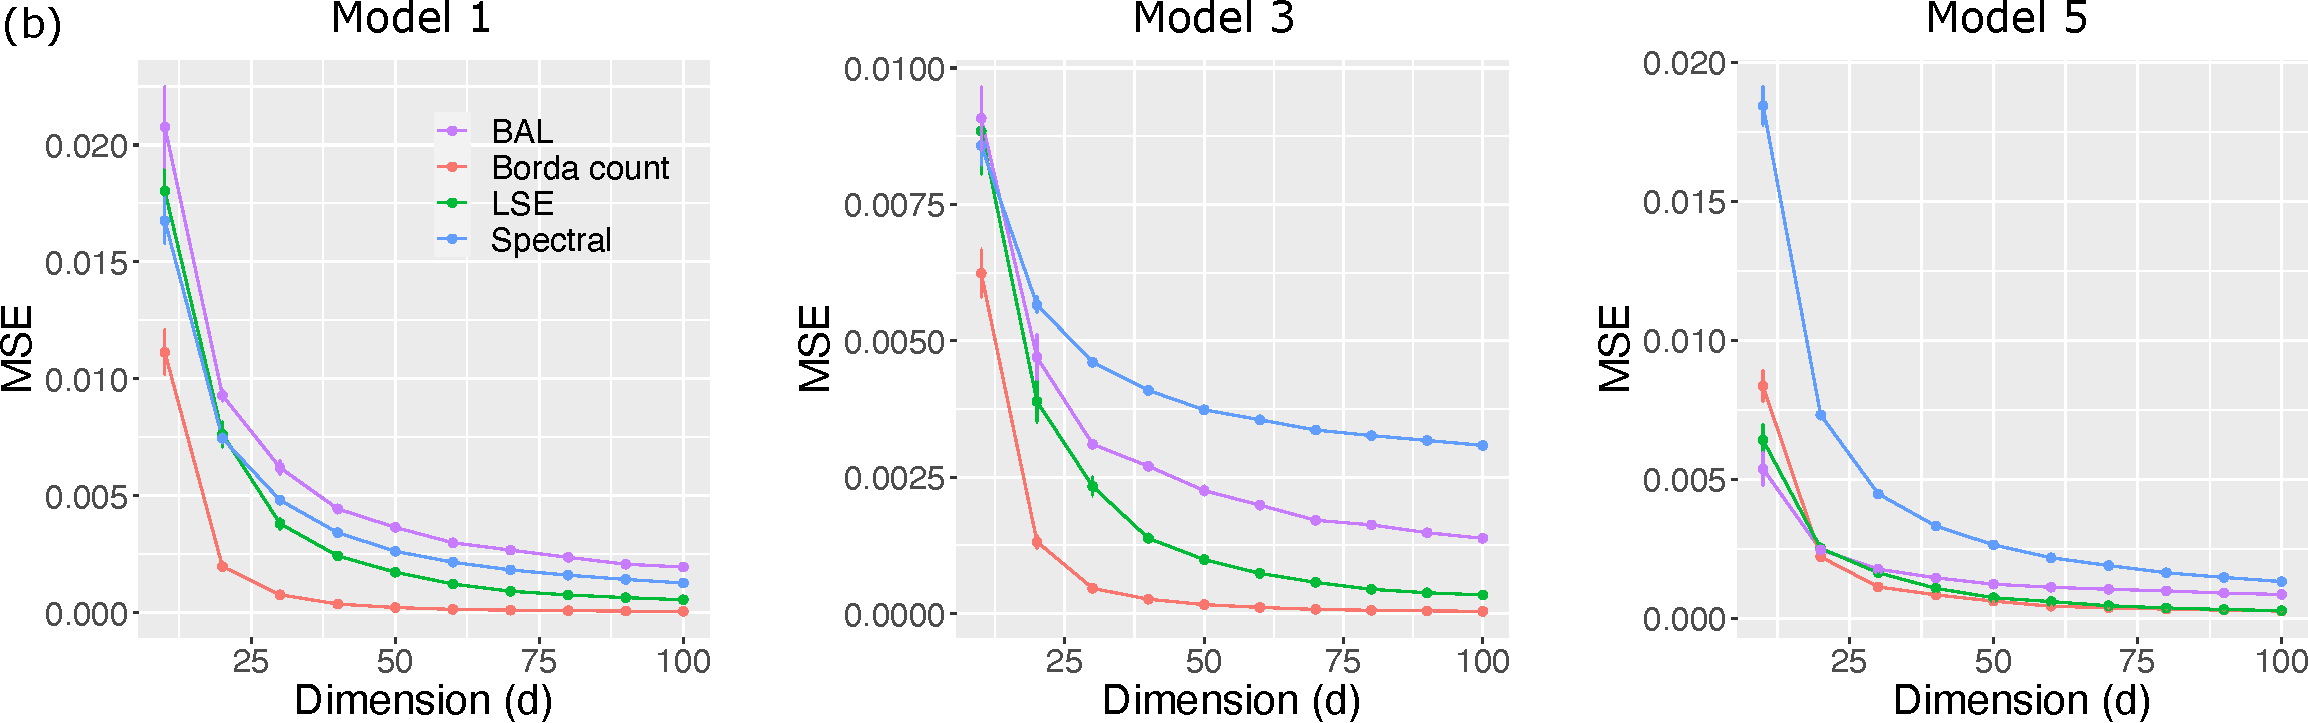
\includegraphics[width = \textwidth]{figure/altdim_binary.pdf}   
    \end{subfigure}
    \caption{MSE versus the tensor dimension based on different estimation methods. Columns 1-3 consider the Models 1, 3, and 5 in Table~\ref{tb:md} respectively. Panel (a) is for continuous tensors, whereas (b) is for the binary tensors.}
    \label{fig:method}
\end{figure}


\begin{figure}[ht]
    \centering
    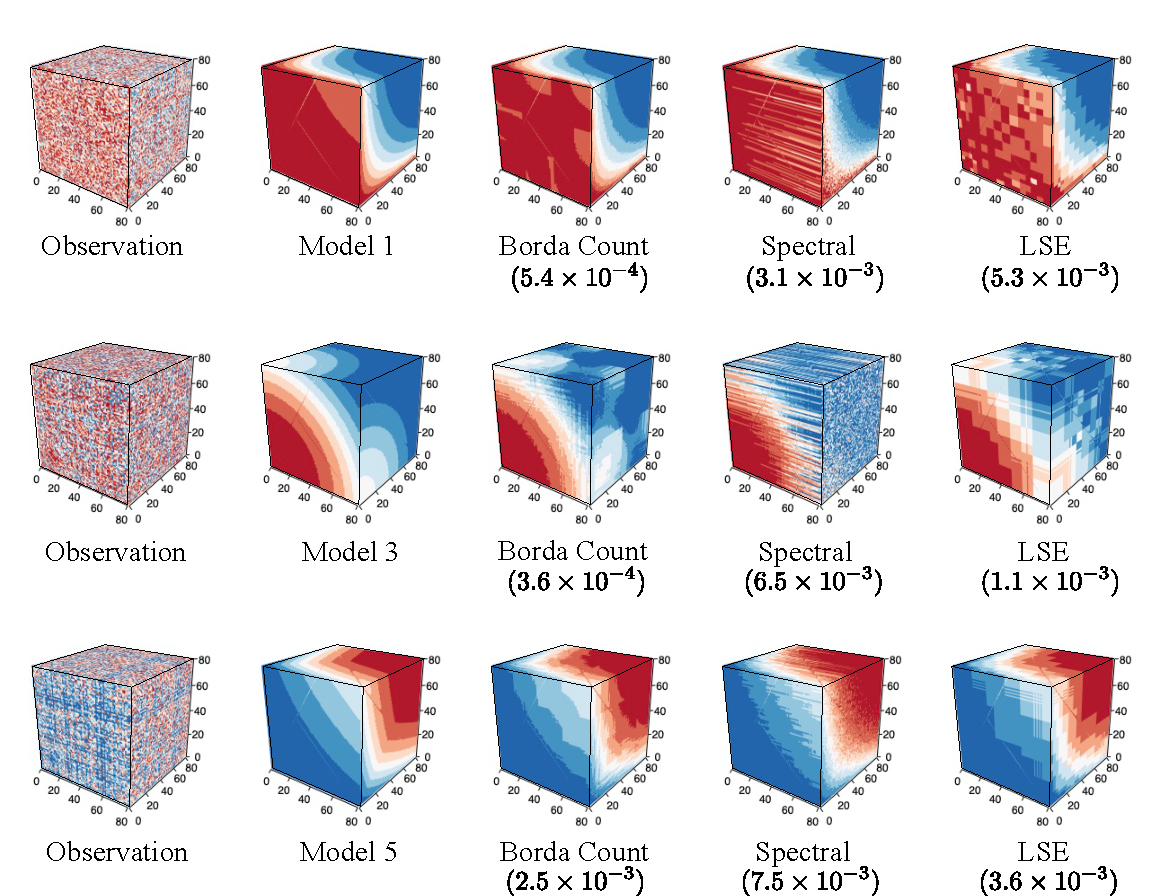
\includegraphics[width =0.9\textwidth]{figure/vfinal.pdf}
    \caption{Performance comparison among different methods. The observed data tensors, true signal tensors, and estimated signal tensors are plotted for Models 1, 3 and 5 in Table~\ref{tb:md} with fixed dimension $d = 80$. Numbers in parenthesis indicate the mean squared error.}
    \label{fig:contim}
\end{figure}


\paragraph{Comparison with alternative methods.} We compare our method ({\bf \small Borda Count}) with several popular alternative methods. 
\begin{itemize}[wide, labelwidth=0pt, labelindent=0pt,itemsep=0ex]
    \item  Spectral method ({\bf \small Spectral})~\citep{xu2018rates} that performs universal singular value thresholding~\citep{chatterjee2015matrix} on the unfolded tensor.
    \item Least-squares estimation ({\bf \small LSE}) \citep{gao2015rate} which solves the optimization problem \eqref{eq:lseopt} with constant block approximation ($\ell=0$) based on spectral $k$-means. We extend the matrix-based biclustering algorithm to higher-order tensors~\citep{han2020exact}. 
    \item Least-squares estimation ({\bf \small BAL}) \citep{balasubramanian2021nonparametric} which solves the optimization problem \eqref{eq:lseopt} with constant block approximation ($\ell=0$). This tensor-based algorithm is only available for binary observations because it uses count-based statistics. Therefore, we only use this algorithm for the Bernoulli model.
\end{itemize}
We choose degree-2 polynomial approximation as our theorems suggested, and vary tensor dimension $d\in\{10,\ldots,100\}$ under each model configuration. For {\bf \small Borda Count} and {\bf \small LSE}, we choose the block numbers that achieve the best performance in the corresponding outputs. For {\bf \small Spectral} method, we set the hyperparameter (singular-value threshold) that gives the best performance. 


Figure~\ref{fig:method} shows that our algorithm {\bf \small Borda Count} achieves the best performance in all scenarios as the tensor dimension increases. The poor performance of {\bf \small Spectral} can be explained by the loss of multilinear structure in the tensor unfolding procedure. The sub-optimality of {\bf \small LSE} is possibly due to its limits in both statistics and computations. Statistically, our theorems have shown that constant block approximation results in sub-optimal rates compared to polynomial approximation. Computationally, the least-squares optimization~\eqref{eq:lseopt} is highly non-convex and computationally unstable. 
Figure~\ref{fig:contim} displays true signal tensors of three models and corresponding observed tensors of dimension $d = 80$ with Gaussian noise. We use oracle permutation $\pi$ to obtain the estimated signal tensor from the estimated permuted signal tensor $\hat\Theta\circ\hat\pi$ for the better visualization and comparisons. As shown in the figure, we see clearly that our method achieves the best signal recovery, thereby supporting the numerical results in Figure~\ref{fig:method}.
The outperformance of {\bf \small Borda count} demonstrates the efficacy of our method.


\paragraph{Investigation of non-symmetric tensors.}\label{sec:asym}
Our models and techniques easily extend to non-symmetric tensors. We simulate order-3 tensors based on the non-symmetric functions in Table~\ref{tb:md2}. 

\begin{table}[ht]
    \centering
    \begin{tabular}{c|c}
        Model ID  &  $f(x,y,z)$  \\\hline
        1 &    $xy+z$ \\
        2&  $x^2+y +yz^2$\\
        3 & $x(1+\exp(-3(x^2+y^2+z^2)))^{-1}$\\
        4 & $\log(1+\max(x,y,z)+x^2+yz)$ \\
        5 &  $\exp\left(-x-\sqrt{y}-z^3\right)$
    \end{tabular}
    \caption{List of non-symmetric smooth functions in simulation.}
    \label{tb:md2}
\end{table}


We fix the tensor dimension ${30\times40\times 50}$ and assume that the noise tensors are from Gaussian distribution. Similar to other simulations, the hyperparameters are chosen via cross-validation that give the best accuracy for each method. Table~\ref{tb:hyper} summarizes the choice of hyperparameters.  Table~\ref{tb:asymresult} compares the MSEs from repeated simulations based on different methods under Models 1-5 (see Table~\ref{tb:md2}). We find that Borda count estimation outperforms all alternative methods for non-symmetric tensors. The results demonstrate the applicability of our method to general tensors. 


\begin{table}[ht]
    \centering
    \begin{tabular}{c|c|c|c|c|c}
        Method &  Model 1 & Model 2 & Model 3& Model 4 & Model 5  \\\hline
        Borda count &   (2,1,2)&(1,2,2)& (1,3,3) &(2,1,2)&(1,4,4)\\
        LSE &(6,2,3)&(8,5,8)&(6,9,6)&(9,5,6)&(7,9,3)\\
        Spectral & (1,24)&(3,48)&(1,48)&(1,28)&(1,22)
    \end{tabular}
    \caption{Hyperparameters for the methods under Models 1-5 in Table~\ref{tb:md2}. For {\bf \small Borda count} and {\bf \small LSE} methods, the values in the table indicate the number of blocks. For {\bf \small Spectral} method, the first value indicates the tensor unfolding mode, while the second one represents the singular value threshold.}
    \label{tb:hyper}
\end{table}


\begin{table}[ht]
    \centering
    \begin{tabular}{c|c|c|c|c|c}
        Method &  Model 1 & Model 2 & Model 3& Model 4 & Model 5  \\\hline
        Borda count &  {\bf 0.57 (0.01)}&{\bf 0.51 (0.02)}& {\bf0.87 (0.02)} &{\bf1.02 (0.02)}& {\bf2.56 (0.21)}\\
        LSE &23.58 (0.03)&7.70 (0.04)&9.45 (0.05)&3.29 (0.05)&9.93 (0.03)\\
        Spectral & 10.76 (0.06)&10.64 (0.05)&6.27 (0.05)&10.90 (0.06)&5.24 (0.04)
    \end{tabular}
    \caption{MSEs from 20 repeated simulations based on different methods. All numbers are displayed on the scales $10^{-3}$. Standard errors are reported in parenthesis.}
    \label{tb:asymresult}
\end{table}



\subsection{Applications to Chicago crime data}

\begin{figure}[ht!]
    \centering
    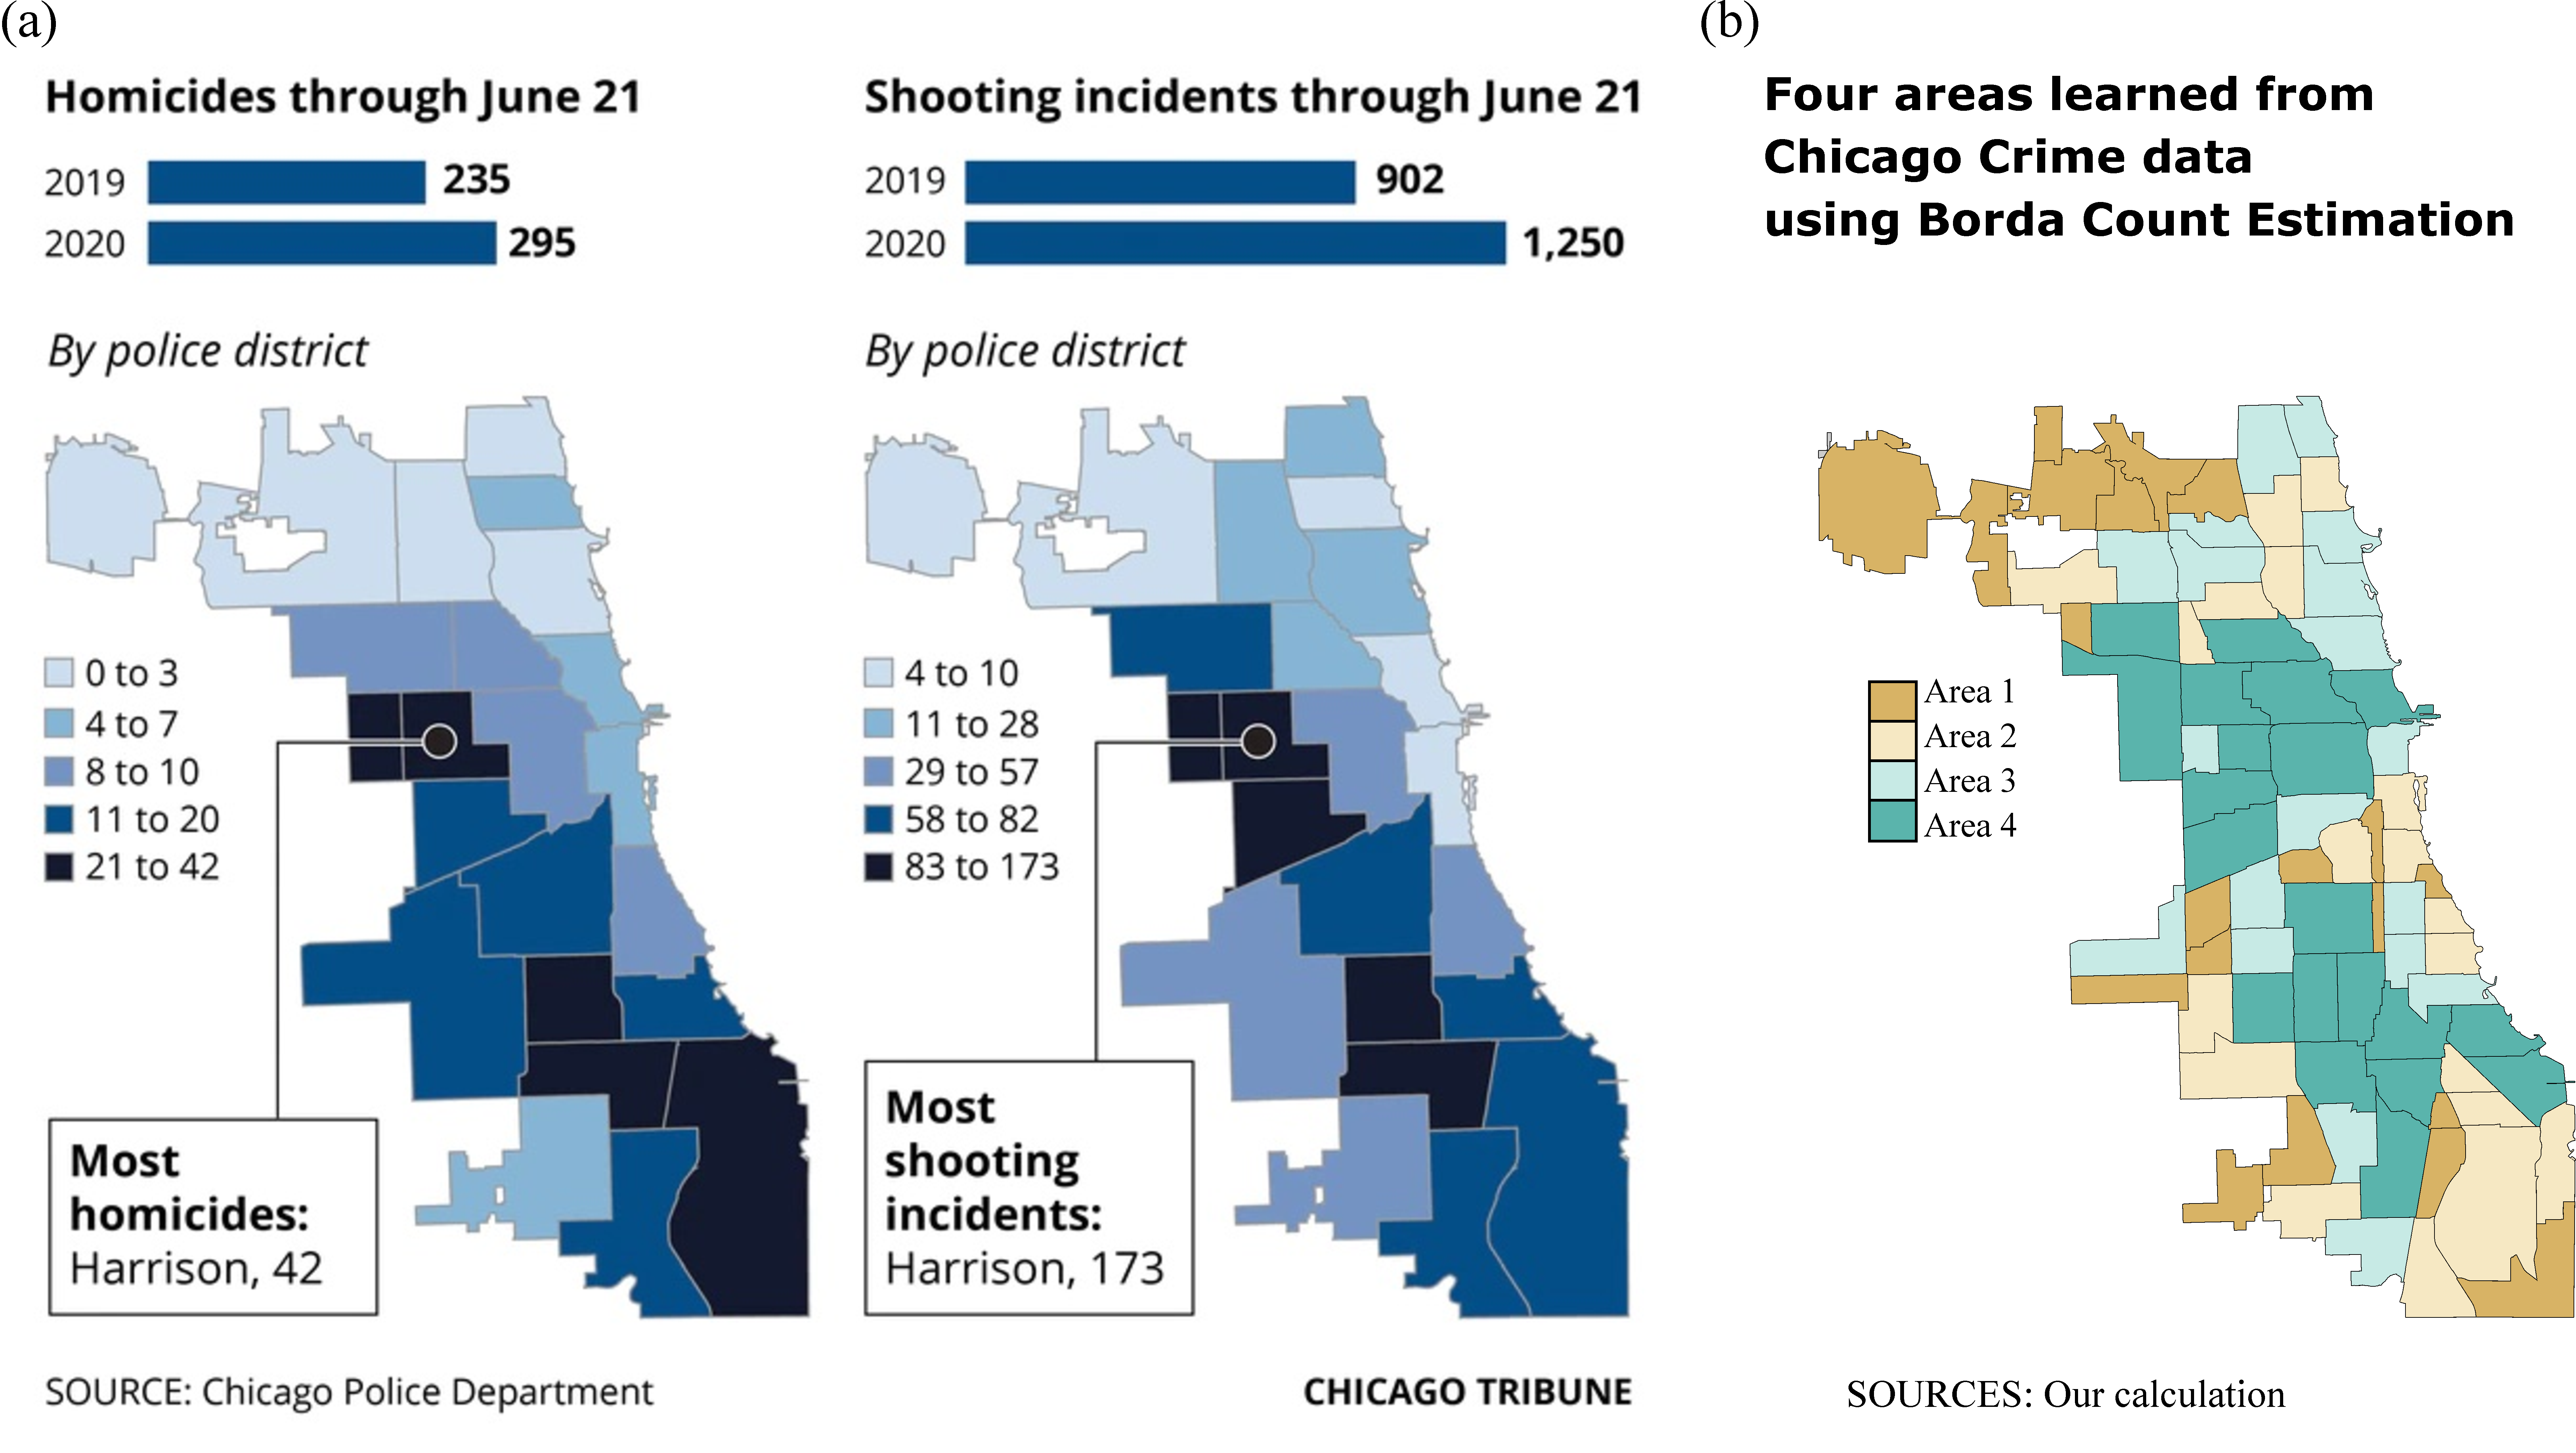
\includegraphics[width = \textwidth]{figure/crimecompare.pdf}
    \caption{Chicago crime maps. Figure(a) is the benchmark map based on homicides and shooting incidents in community areas in Chicago~\citep{Jeremy.2020}. Figure(b) shows the four clustered areas learned from 32 crime types using our method.}
    \label{fig:area}
\end{figure}


Chicago crime dataset consists of crime counts reported in the city of Chicago, ranging from January 1st, 2001 to December 11th, 2017. The observed tensor is an order-3 tensor with entries representing the log counts of crimes from 24 hours, 77 community areas, and 32 crime types. We apply our Borda count method to Chicago crime dataset. Because the data tensor is non-symmetric, we allow different number of blocks across the three modes. Cross validation result suggests the $(k_1,k_2,k_3)=(6,4,10)$, representing the block number for crime hours, community areas, and crime types, respectively.


\begin{figure}[ht!]
    \centering
    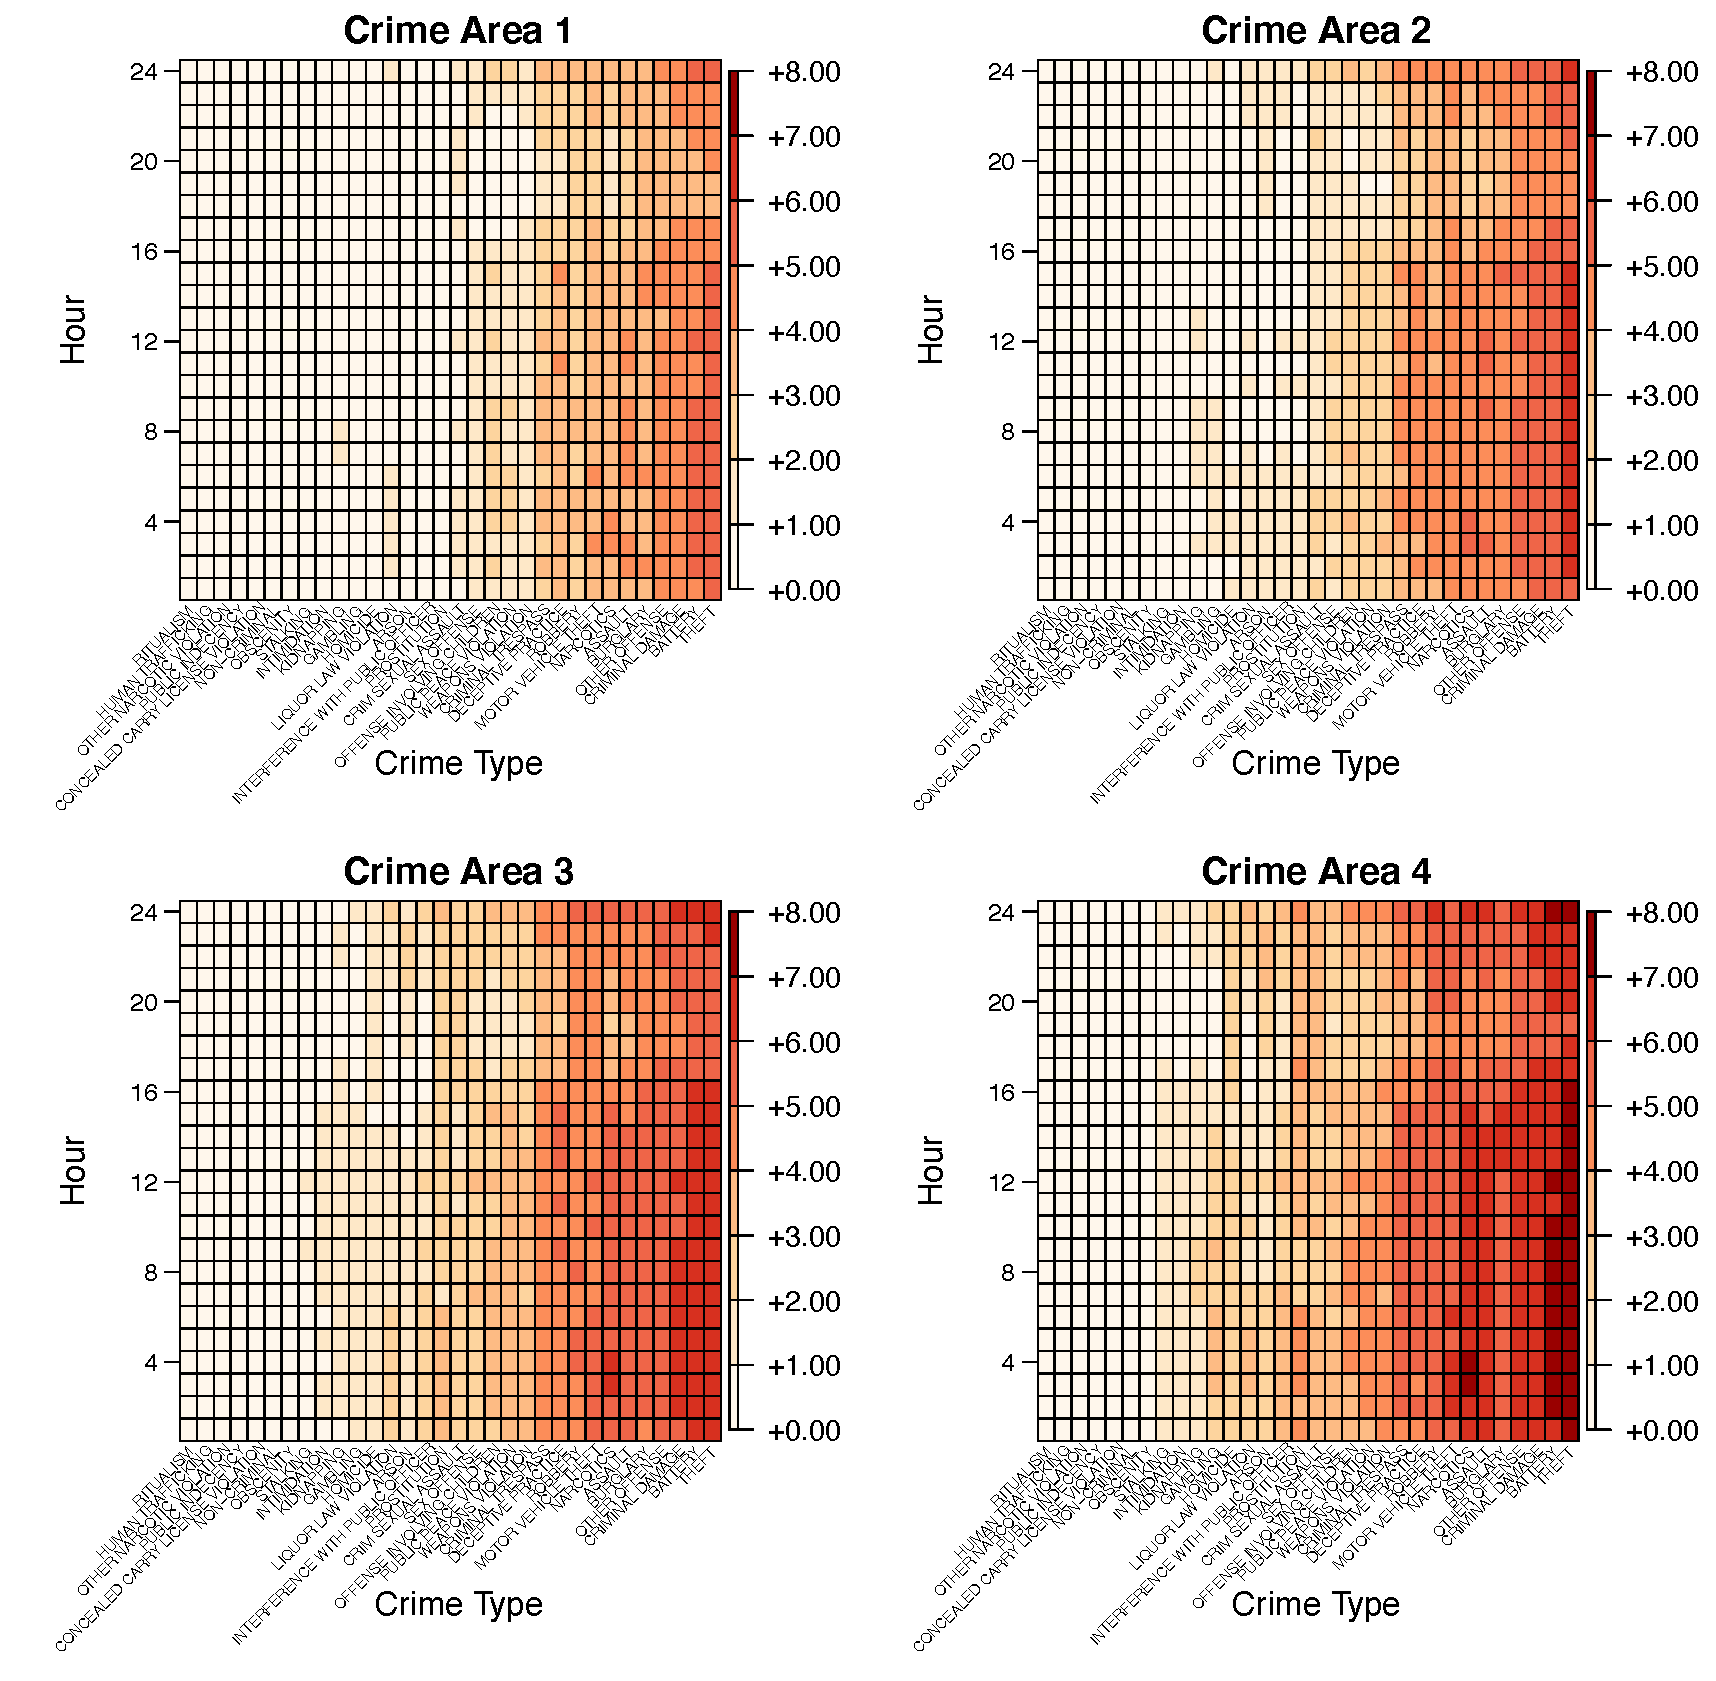
\includegraphics[width = \textwidth]{figure/CrimeA.pdf}
    \caption{Averaged log counts of crimes according to crime types, hours, and the four areas estimated by our Borda count algorithm. We plot the estimated signal tensor entries averaged within four areas in the heatmap.}
    \label{fig:crimeA}
\end{figure}

We first investigate the four community areas obtained from our Borda count algorithm.  Figure~\ref{fig:area}(b) shows the four areas overlaid on the Chicago map. Interestingly, we find that the clusters are consistent with actual locations, even though our algorithm did not take any geographic information such as longitude or latitude as inputs. In addition, we compare the cluster patterns with benchmark maps based on homicides and shooting incidents in Chicago shown in Figure~\ref{fig:area}(a). We find that our clusters share similar geographical patterns with Figure~\ref{fig:area}(a). The results demonstrate the power of our approach in detecting meaningful pattern from tensor data. 




Then, we examine the denoised signal tensor obtained from our method and analyze the trends between crime types and crime hours by the four community areas in Figure~\ref{fig:area}(b). Figure~\ref{fig:crimeA} shows the averaged log counts of crimes according to crime types and crime hours by four areas. We find that the major difference among four areas is the crime rates. Area 4 has the highest crime rates,  and the crime rates monotonically decrease from Area 4 to Area 1. The variation in crime rates across hour and type, nevertheless, exhibits similarity among the four areas. For example, Figure~\ref{fig:crimeA} shows that the number of crimes increases hourly from 8 p.m., peaks at night hours, and then drops to the lowest at 6 p.m. 
The identified similarities and differences among the four community areas highlight the interpretability of our method in real data.

\begin{table}[htp!]
    \centering
    \begin{tabular}{c|c|c}
         &  Constant block model & Permuted smooth tensor model \\\hline
         
        MSE &   0.399 (0.009) &  0.283 (0.006)\\
        Block number &    $(7,11,10)$  & $(6,4,10)$
    \end{tabular}
    \caption{Performance comparison in Chicago data analysis. Reported MSEs are averaged
over five runs of cross-validation, with 20\% entries for testing and 80\% for training, with standard
errors in parentheses. Block number is set to achieve the best prediction performance.}\label{tab:MSE}
\end{table}

Finally, we compare the prediction performance based on constant block model and our permuted smooth tensor model. Notice that constant block model uses $\ell=0$ approximation, whereas our permuted smooth tensor model uses $\ell=2$ approximation. Table~\ref{tab:MSE} shows the mean squared error over five runs of cross-validation, with 20\% entries for testing and 80\% for training. We find that the permuted smooth tensor model substantially outperforms the classical constant block models. We emphasize that our method does not necessarily assume the block structure. The comparison supports our premises that permuted smooth tensor model with polynomial approximation performs better than common constant block models in this application. 




\section{Conclusion and Discussions}\label{sec:discussion}
We have presented a suite of statistical theory, estimation methods, and data applications for permuted smooth tensor models. Two estimation algorithms are proposed with accuracy guarantees: the (statistically optimal) least-squares estimation and the (computationally tractable) Borda count estimation. In particular, we establish an interesting phase transition phenomenon with respect to the critical smoothness level. We demonstrate that a block-wise polynomial of order $(m-2)(m+1)/2$ is sufficient and necessary for accurate recovery of order-$m$ tensors, in contrast to earlier beliefs on constant block approximation. Experiments demonstrate the effectiveness of both theoretical findings and algorithms. 

There are several possible extensions from our work. The theory in this paper assumes symmetry on the signal tensor $\Theta$ for simplicity of exposition. In fact, all our results naturally extend to non-symmetric signal tensors. A non-symmetric tensor $\Theta\in\bbR^{d_1\times \cdots\times d_m}$ can be represented by $\Theta(i_1,\ldots,i_m) = f\left({\pi_1(i_1)\over d_1},\ldots,{\pi_m(i_m)\over d_m}\right)$, where $\pi_\ell\colon [d_\ell]\rightarrow [d_\ell]$ is the latent permutation for each mode $\ell\in[m]$, and the function $f$ is a smooth but non-symmetric function. Under the condition that $d_1,\ldots, d_m$ are asymptotically of the same order, similar estimation algorithms and theoretical accuracy guarantees still hold true.  

Our framework of block-wise polynomial approximation can be extended to allow other nonparametric techniques, including B splines, smoothing splines, kernel regression, wavelets, etc. We choose to use polynomial basis because of its simplicity. The parsimony allows us to establish the insights on critical smoothness level $ (m-2)(m+1)/2$. For example, our result suggests that quadratic splines are enough for accurate estimation of order-3 tensors. One can combine our approach with the modern trend filtering techniques~\citep{tibshirani2014adaptive,ortelli2019prediction},
\[
\hat f =\argmin_{f}\sum_{(i_1,i_2,i_3)}\left(\tY(\hat \pi(i_1),\hat \pi(i_2),\hat \pi(i_3))-f\left({i_1\over d},{i_2\over d},{i_3\over d}\right)\right)^2+\lambda \norm{{\boldsymbol \nabla}_2 f},
\]
where $\norm{{\boldsymbol \nabla}_2 f}$ represents total variation of second order difference. The case of $m=2$ (matrix) reduces to the total variation smoothing in graphons~\citep{chan2014consistent}. For general order-$m$ tensors, our theory provides a principle of guidance for the order of smoothness needed. Exploiting the benefits and properties of various nonparametric fitting techniques for general tensor models warrants future research.

Finally, our current approach assumes no randomness in the signal tensor $\Theta$. One can also extend the generative model to allow random designs, where the signal tensor is represented by $\Theta(i_1,\ldots,i_m)=f(x_{i_1},\ldots,x_{i_m})$ with $(x_i)_{i=1}^d$ i.i.d.\ randomly drawn from certain distribution. Similar techniques have been developed for graphons and hypergraphons~\citep{chan2014consistent,gao2015rate,klopp2017oracle,balasubramanian2021nonparametric}. The two choices of designs lead to different analysis in the same spirit as random- vs. fixed-designs in nonparametric regression. Extending our theory to random design is an interesting question for future research.


%\section*{Acknowledgements}
%This research is supported in part by NSF grants DMS-1915978, DMS-2023239, and funding from the Wisconsin Alumni Research foundation.

\bibliographystyle{Chicago.bst}
\bibliography{tensor_wang}

\clearpage
\appendix
\section*{Appendix}
The appendix includes extra simulation results, proof of main theormes, and technical lemmas. 




\renewcommand{\thefigure}{S\arabic{figure}}
\setcounter{figure}{0}   
\renewcommand{\thetable}{S\arabic{table}}
\setcounter{table}{0}   

\section{Extra numerical results}
\subsection{Results for Models 2 and 4 in Table~\ref{tab:comp}}\label{sec:extra}
We first present simulation results for Models 2 and 4 omitted in Section~\ref{sec:sim}. Figure~\ref{fig:extrav} compares the estimation performance among the {\bf \small Borda count, LSE}, and {\bf \small Spectral methods}. We find that our Borda count algorithm outperforms others in both models. The first two columns in Figure~\ref{fig:extrasim1} show the impact of the number of blocks $k$ and degree of polynomial $\ell$ for the approximation with fixed dimension $d = 100$. Similar to results for Models 1, 3 and 5 in the main paper, we find the optimal $k$ balances the trade-off between approximation error and signal tensor estimation error within each block. The last two columns compare our {\bf \small Borda count} with other alternative methods. We find that our method still outperforms {\bf \small LSE} and {\bf \small Spectral} in all scenarios under Models~2 and~4.

\begin{figure}[h!]
    \centering
    \begin{subfigure}[b]{\textwidth}
    \vspace{0.5cm}
    
    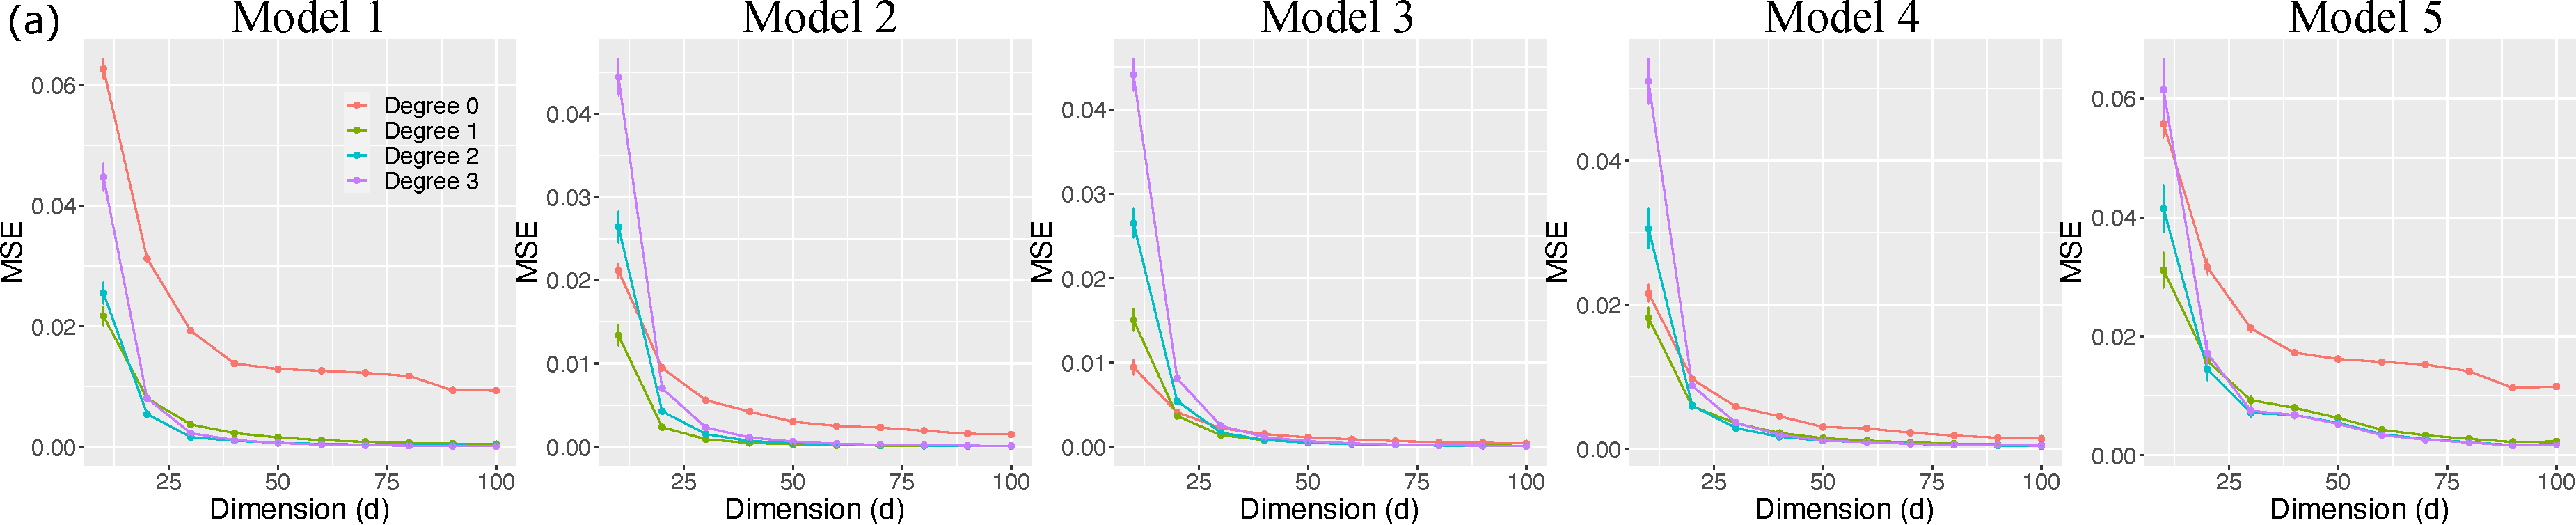
\includegraphics[width = \textwidth]{figure/deg_dim_c.pdf} 
    \vspace{0cm}
    \end{subfigure}
    \begin{subfigure}[b]{\textwidth}
    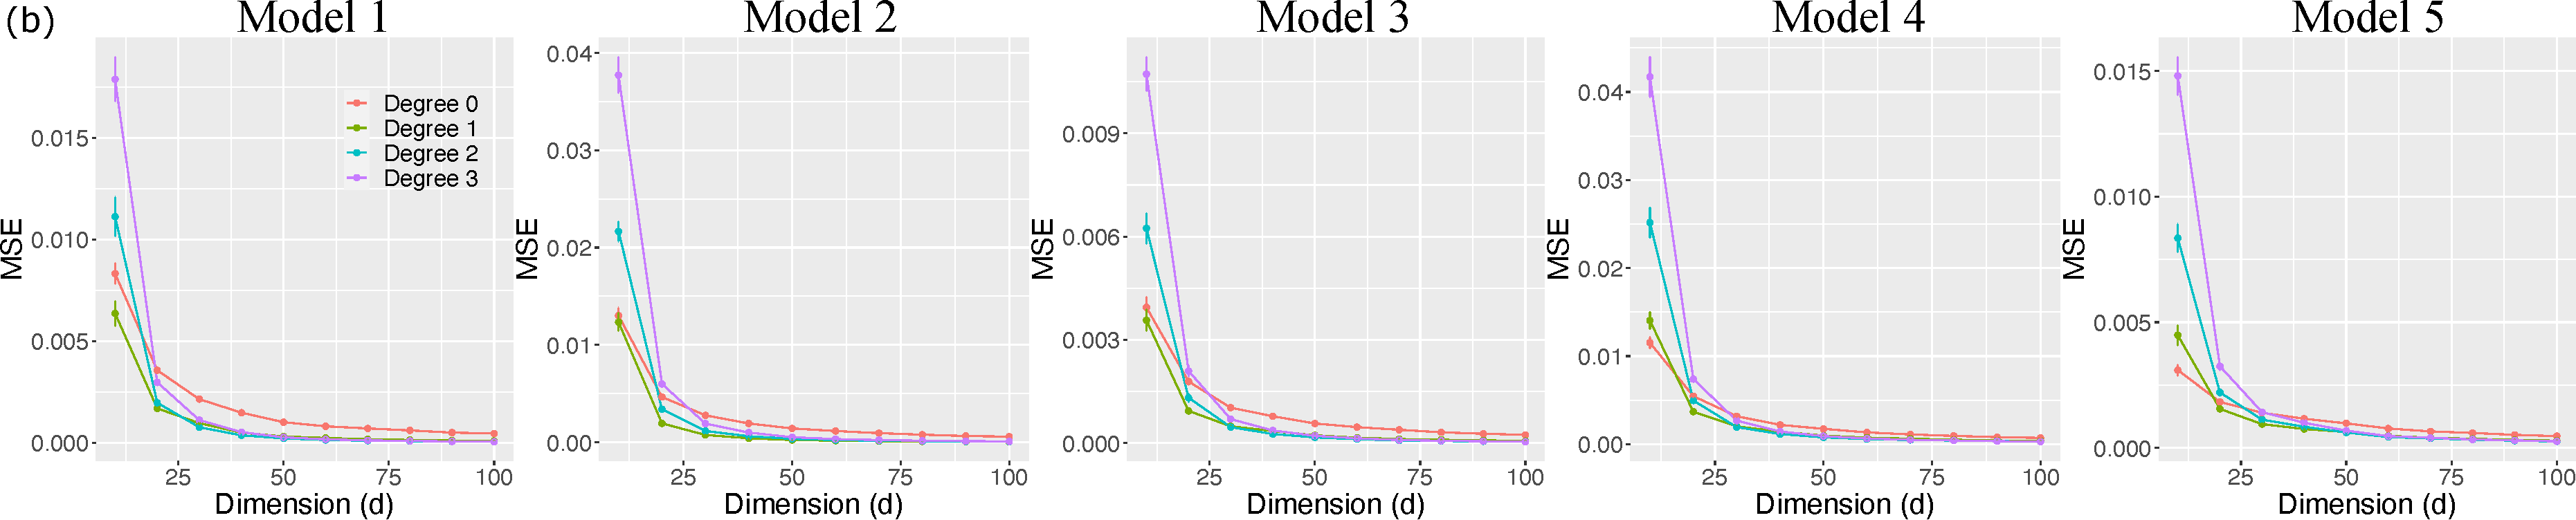
\includegraphics[width =\textwidth]{figure/deg_dim_b.pdf}    
    \end{subfigure}
    \caption{MSE versus the tensor dimension based on different polynomial approximations. Columns 1-5 consider the Models 1-5 in Table~\ref{tb:md} respectively. Panel (a) is for continuous tensors, whereas (b) is for the binary tensors.}
    \label{fig:degdim}
\end{figure}


\begin{figure}[htp!]
    \centering
    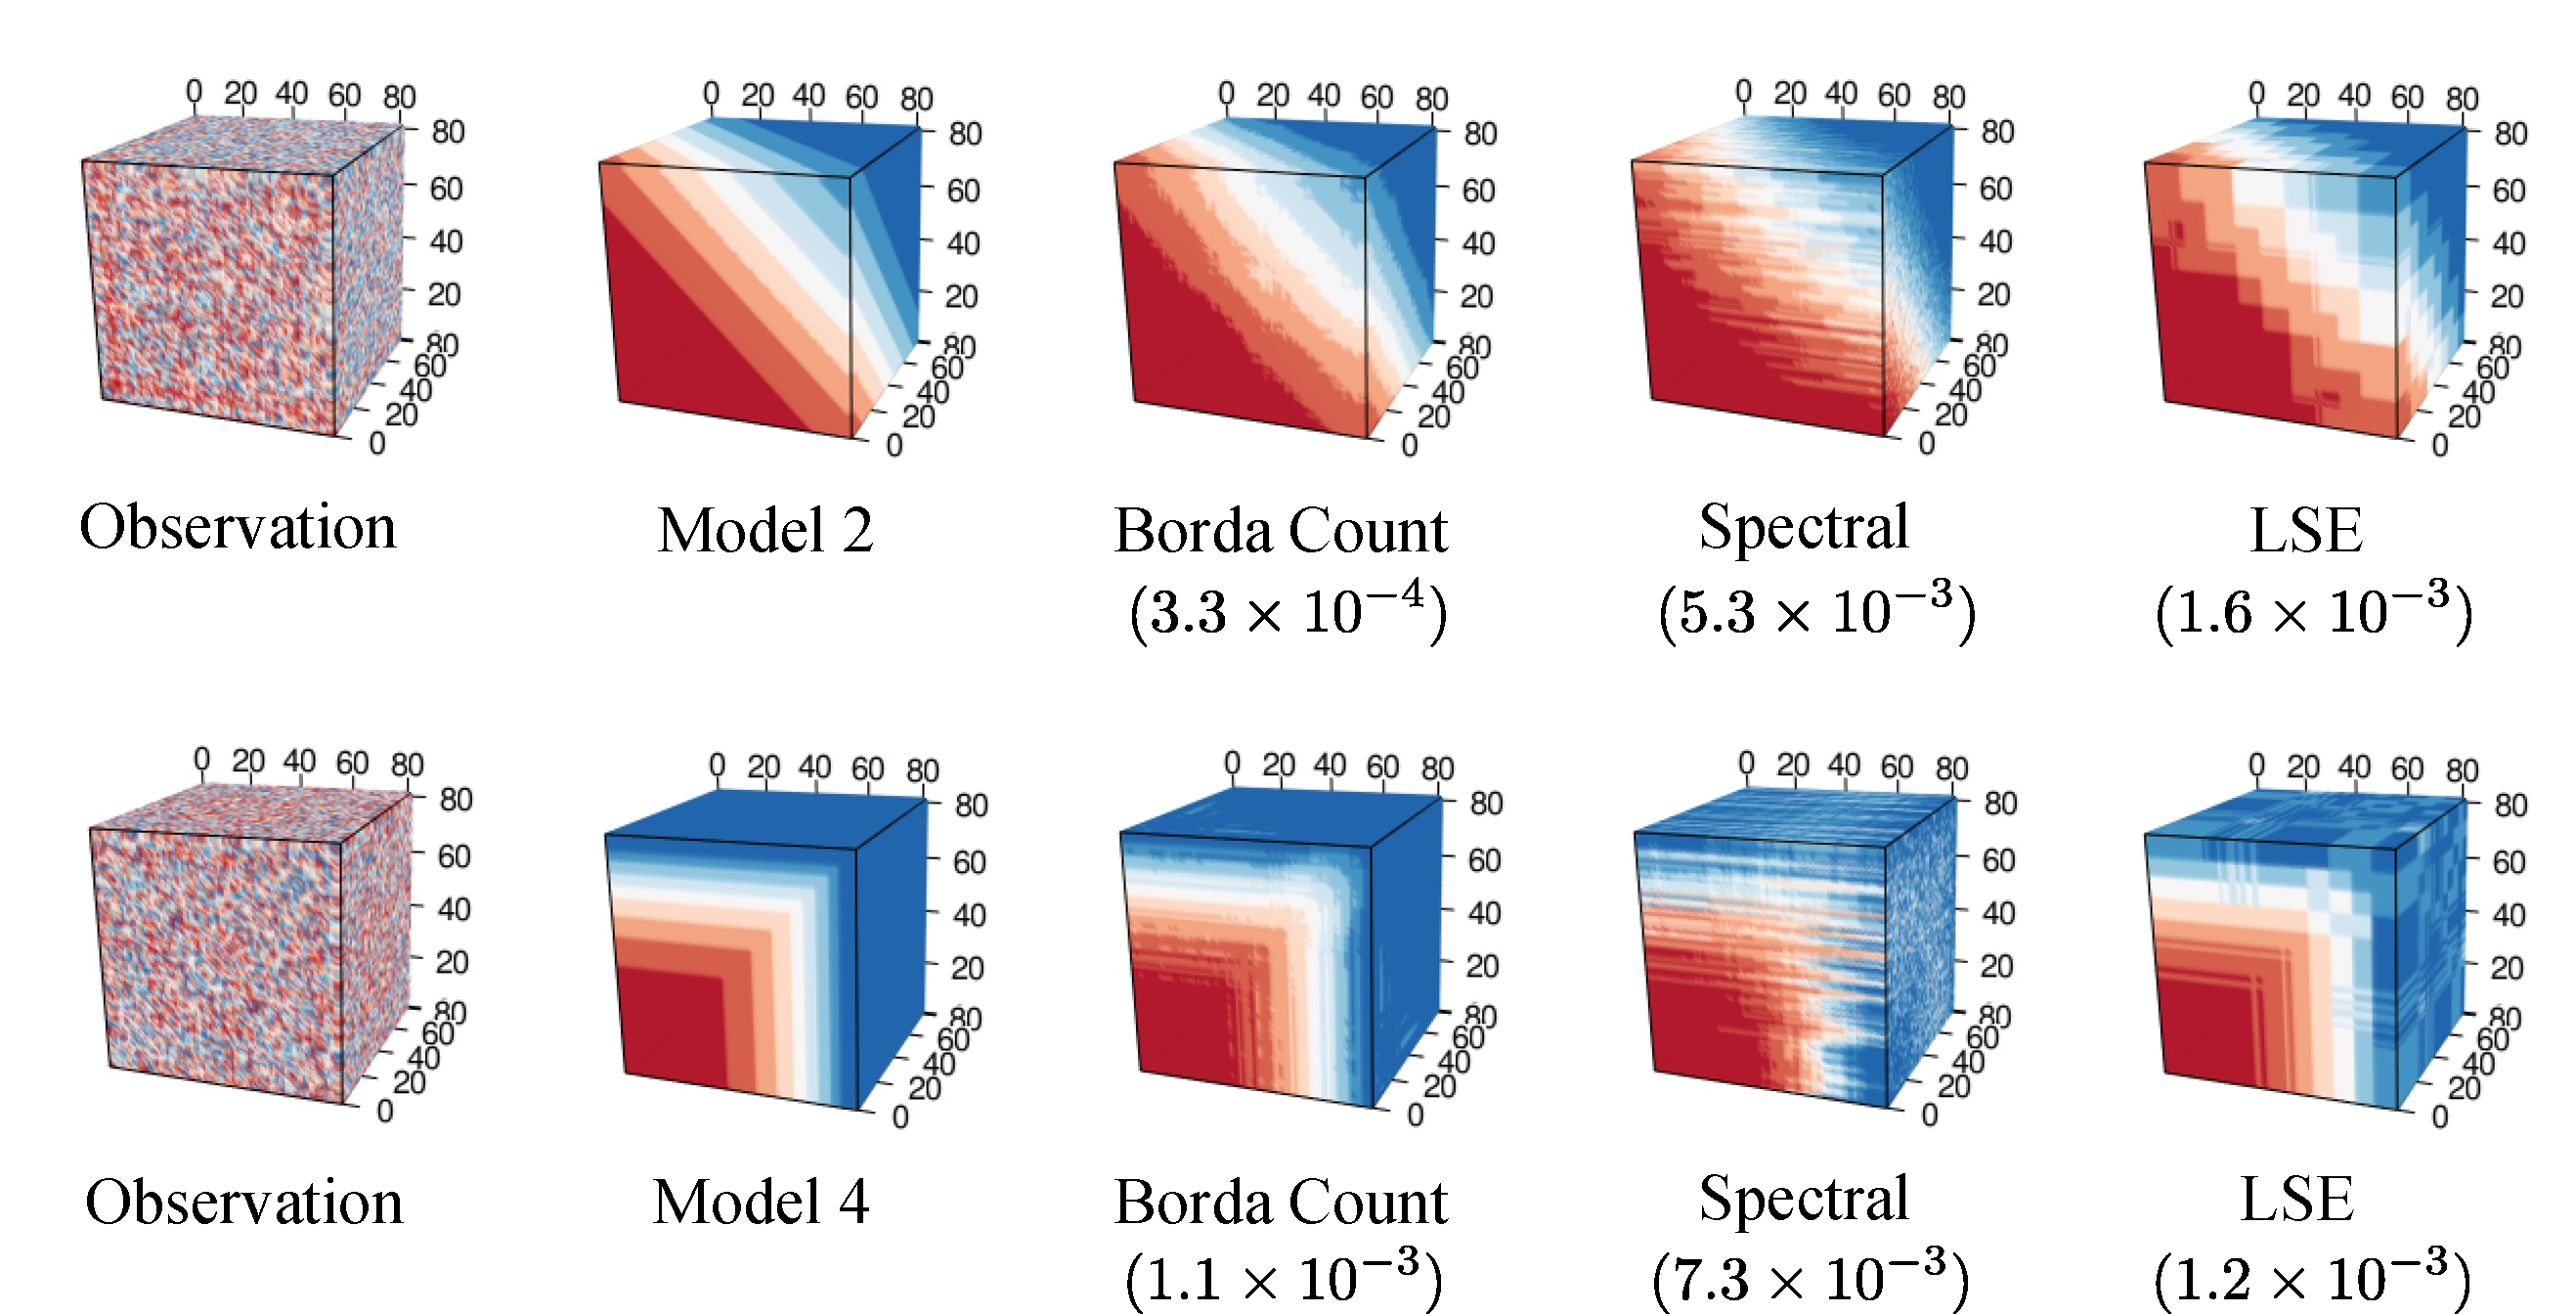
\includegraphics[width =0.9\textwidth]{figure/extravfinal.pdf}
    \caption{Performance comparison between different methods. The observed data tensors, true signal tensors, and estimated signal tensors are plotted for Models 2 and 4 in Table~\ref{tb:md} with fixed dimension $d = 80$. Numbers in parenthesis indicate the mean squared error.}
    \label{fig:extrav}
\end{figure}


\begin{figure}[htp!]
    \centering
    \begin{subfigure}[b]{\textwidth}
    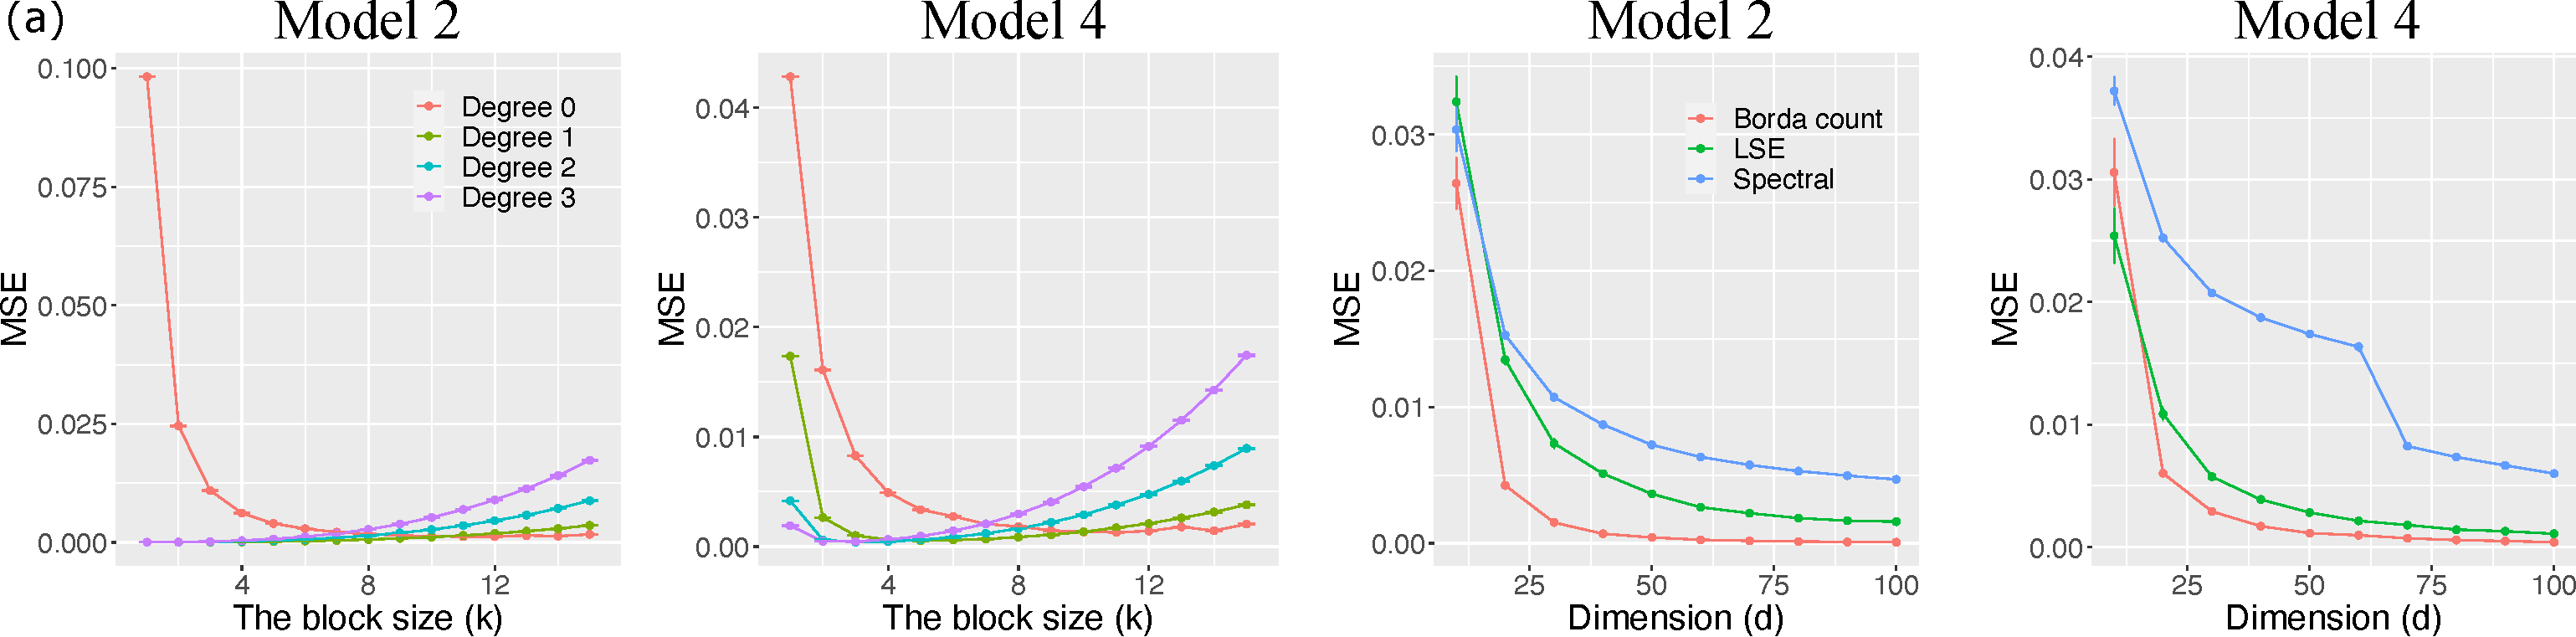
\includegraphics[width = \textwidth]{figure/extra_conti.pdf}  
        \vspace{0cm}
    \end{subfigure}
    \begin{subfigure}[b]{\textwidth}
    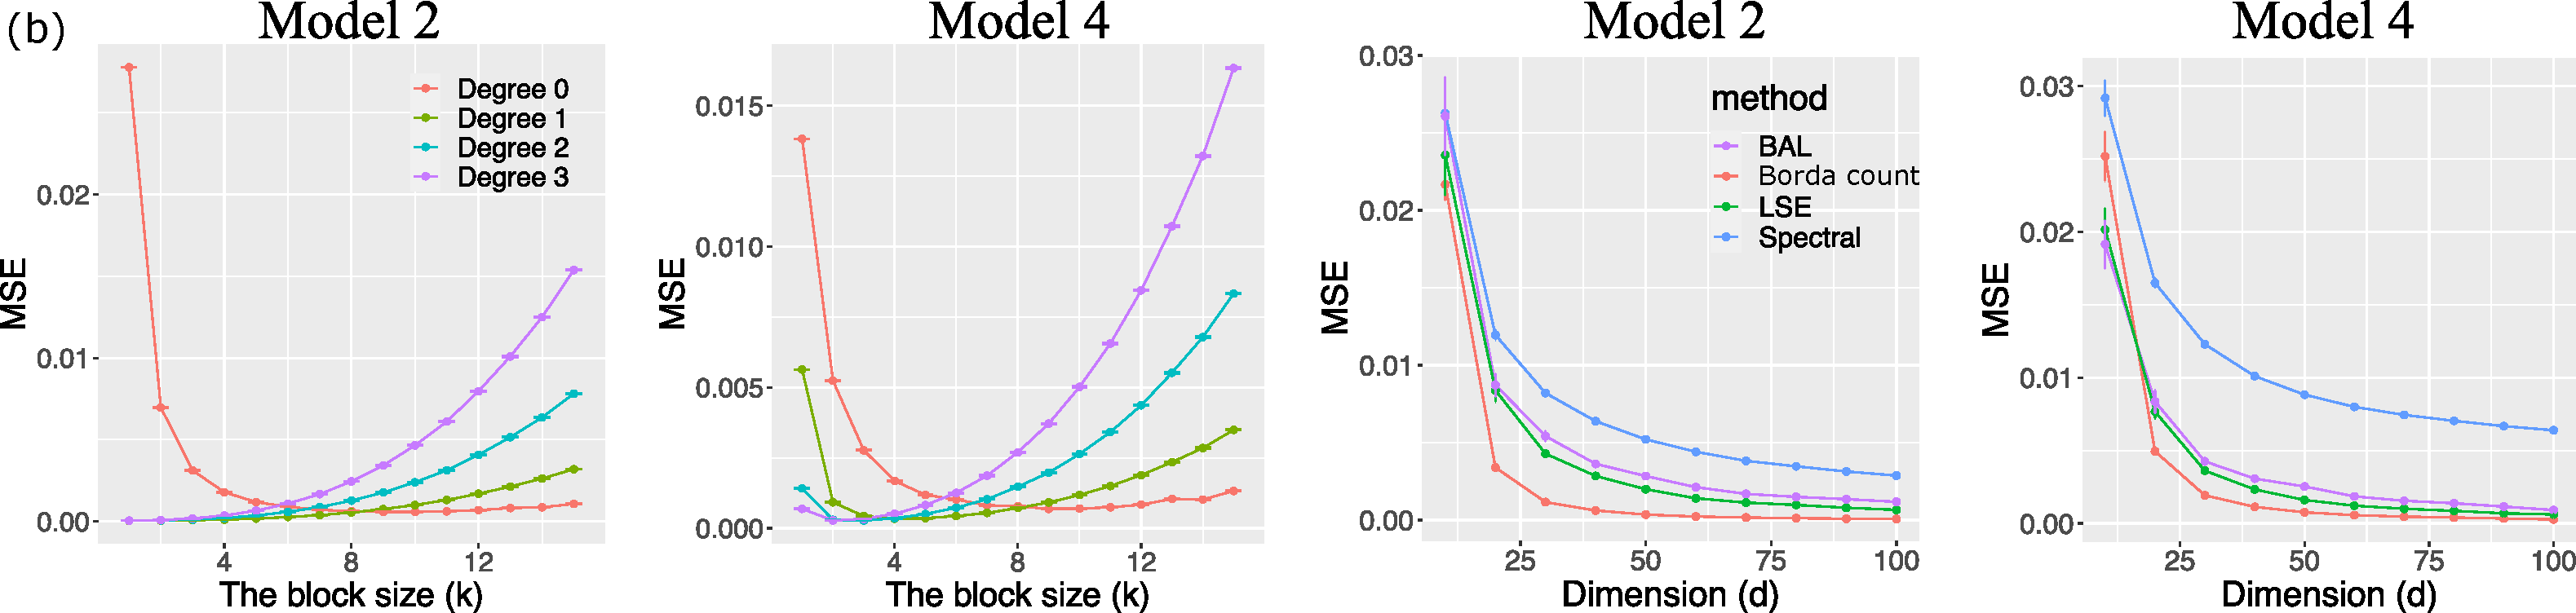
\includegraphics[width = \textwidth]{figure/extra_binary.pdf}    
    \end{subfigure}
    \caption{Simulation results for Models 2 and 4 in Table~\ref{tb:md}. Columns 1-2 plots MSE versus the number of blocks for different polynomial approximation, while Columns 3-4 shows the MSE versus the tensor dimension according to estimation methods. Panel (a) is for continuous tensors, whereas (b) is for the binary tensors.}
    \label{fig:extrasim1}
\end{figure}


\subsection{Extra results on Chicago crime data analysis}\label{subsec:chicago}
We investigate the ten groups of crime types clustered by our method. Table~\ref{tb:crimetb} shows that the clustering captures the similar type of crimes. For example, group 2 consists of misdemeanors such as public indecency, non-criminal, and concealed carry license violation, while group 6 represents sex-related offenses such as prostitution, sex offense, and crime sexual assault.

\begin{table}[ht!]
    \centering
    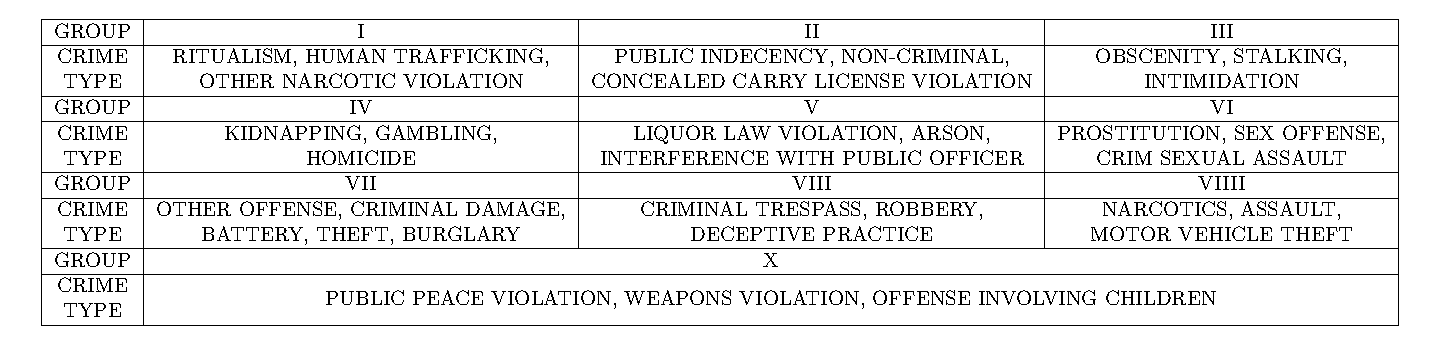
\includegraphics[width = \textwidth]{figure/crimetable.pdf}
    \caption{Groups of crime types learned based on the Borda count estimation.}
    \label{tb:crimetb}
\end{table}


\section{Proofs of main theorems}\label{app:theorem}

Here, we provide proofs of the theoretical results presented in Sections~\ref{sec:tba}-\ref{sec:borda}. 

\subsection{Proof of Lemma~\ref{lem:approx}}
\begin{proof}
Recall that we denote $\tE_k$ as the $m$-way partition
\begin{align}
    \tE_k = \{\bigtimes_{a=1}^m z^{-1}(j_a)\colon (j_1,\ldots,j_m)\in [k]^m\}, 
\end{align}
where $z\colon [d]\rightarrow[k]$ is the canonical clustering function such that $z(i) = \lceil ki/d\rceil,$ for all $i \in[d]$, and we use the shorthand $\bigtimes_{a=1}^m$ to denote the Cartesian product of $m$ sets. For a given partition  $ \bigtimes_{a=1}^m z^{-1}(j_a)\in\tE_k$, fix any index  $(i_1^0,\ldots,i_m^0)\in \bigtimes_{a=1}^m z^{-1}(j_a)$. Then, we have 
\begin{align}\label{eq:ind}
\|(i_1,\ldots,i_m)-(i_1^0,\ldots,i_m^0)\|_\infty \leq \frac{d}{k},
\end{align} 
for all $(i_1,\ldots,i_m)\in \bigtimes_{a=1}^m z^{-1}(j_a)$.
We define the block-wise degree-$\ell$ polynomial tensor $\tB$ based on the partition $\tE_k$ as
\begin{align}
    \tB(i_1,\ldots,i_m) = \text{Poly}^{j_1,\ldots,j_m}_{\min(\lfloor \alpha \rfloor,\ell)}\left(\frac{i_1-i_1^0}{d},\ldots\frac{i_m-i_m^0}{d}\right), \quad \text{for all } (i_1,\ldots,i_m)\in \bigtimes_{a=1}^m z^{-1}(j_a),
\end{align}
where $\text{Poly}^{j_1,\ldots,j_m}_{\min(\lfloor \alpha \rfloor,\ell)}$ denotes a degree-$\ell$ polynomial function satisfying
\begin{align}\label{eq:polyapp}
\left|f\left(\frac{i_1}{d},\ldots,\frac{i_m}{d}\right)-\text{Poly}^{j_1,\ldots,j_m}_{\min(\lfloor \alpha \rfloor,\ell)}\left(\frac{i_1-i_1^0}{d},\ldots\frac{i_m-i_m^0}{d}\right)\right|\leq L\left\|\left(\frac{i_1-i_1^0}{d},\ldots,\frac{i_m-i_m^0}{d}\right)\right\|_\infty^{\min(\alpha,\ell+1)},
\end{align}
for all $(i_1,\ldots,i_m)\in \bigtimes_{a=1}^m z^{-1}(j_a).$
Notice that we can always find such polynomial function by $\alpha$-H\"older smoothness of the generative function $f$.
Based on the construction of block-wise degree-$\ell$ polynomial tensor $\tB$, we have 
\begin{align}
   & \frac{1}{d^m}\FnormSize{}{\Theta-\tB}^2\\
=&\ \frac{1}{d^m} \sum_{(i_1,\ldots,i_m)\in[d]^m}|\Theta(i_1,\ldots,i_m)-\tB(i_1,\ldots,i_m)|^2\\
=&\ \frac{1}{d^m}\sum_{(j_1,\ldots,j_m)\in[k]^m}\sum_{(i_1,\ldots,i_m)\in \bigtimes_{a=1}^m z^{-1}(j_a)}\bigg|f\left(\frac{i_1}{d},\ldots,\frac{i_m}{d}\right)-\text{Poly}^{j_1,\ldots,j_m}_{\min(\lfloor \alpha \rfloor,\ell)}\left(\frac{i_1-i_1^0}{d},\ldots,\frac{i_m-i_m^0}{d}\right)\bigg|^2\\
    \lesssim &\ \frac{L^2}{d^m}\sum_{(j_1,\ldots,j_m)\in[k]^m}\sum_{(i_1,\ldots,i_m)\in \bigtimes_{a=1}^m z^{-1}(j_a)} \left\|\left(\frac{i_1-i_1^0}{d},\ldots,\frac{i_m-i_m^0}{d}\right)\right\|_\infty^{2\min(\alpha,\ell+1)}\\
    \leq&\ \frac{L^2}{k^{2\min(\alpha,\ell+1)}},
\end{align}
where the first inequality uses~\eqref{eq:polyapp} and the second inequality is from \eqref{eq:ind}.
\end{proof}




\subsection{Proof of Theorem~\ref{thm:LSE}}\label{sec:proofLSE}
\begin{proof} By Lemma~\ref{lem:approx}, there exists a block-wise polynomial tensor $\tB\in\caliB(k,\ell)$ such that
\begin{equation}\label{eq:approx}
\FnormSize{}{\tB-\Theta}^2\lesssim {L^2d^m\over k^{2\min(\alpha,\ell)}}.
\end{equation}
By the triangle inequality,
\begin{equation}\label{eq:tri}
\FnormSize{}{\hat\Theta^\textup{LSE}\circ\hat\pi^\textup{LSE} -\Theta\circ \pi}^2\leq 2\FnormSize{}{\hat\Theta^\textup{LSE}\circ\hat\pi^\textup{LSE} -\tB\circ \pi}^2+2\underbrace{\FnormSize{}{\tB\circ \pi-\Theta\circ \pi}^2}_{\textup{Lemma~\ref{lem:approx}}}.
\end{equation}
Therefore, it suffices to bound $\FnormSize{}{\hat\Theta^\textup{LSE}\circ\hat\pi^\textup{LSE} -\tB\circ \pi}^2$. By the global optimality of least-square estimator, we have
\begin{align}
\FnormSize{}{\hat\Theta^\textup{LSE}\circ\hat\pi^\textup{LSE} -\tB\circ \pi}&\leq \left\langle {\hat \Theta^\textup{LSE}\circ \hat \pi^\textup{LSE}-\tB\circ \pi \over \FnormSize{}{ \hat \Theta^\textup{LSE}\circ \hat \pi^\textup{LSE}-\tB\circ \pi}},\ \tE+(\Theta\circ \pi-\tB\circ \pi) \right \rangle \\
&\leq \sup_{\pi, \pi'\colon[d]\to[d]}\sup_{\tB, \tB'\in \caliB(k,\ell)} \left\langle {\tB'\circ \pi'-\tB\circ \pi \over \FnormSize{}{\tB'\circ \pi'-\tB\circ \pi}}, \tE \right \rangle+\underbrace{\FnormSize{}{\tB\circ \pi-\Theta\circ \pi}}_{\textup{Lemma~\ref{lem:approx}}}.
\end{align}
Now we bound inner product term. For fixed $\pi,\pi'$, let $\mP$ and $\mP'$ be permutation matrices corresponding to permutations $\pi$ and $\pi'$ respectively. 
We express vectorized block-wise degree-$\ell$ polynomial tensors, $\text{vec}(\tB)$ and $\text{vec}(\tB')$, by discrete polynomial functions. Specifically, denote $\text{vec}(\tB)=\mX\mbeta$ and $\text{vec}(\tB')=\mX\mbeta'$, where $\mX\in\bbR^{d^m\times k^m(k+m)^\ell}$ is a design matrix consisting of $m$-multivaraite degree-$\ell$ polynomial basis over grid design $(1/d,\ldots,d/d)$, $\mbeta$ and $\mbeta'\in\bbR^{k^m(k+m)^\ell}$ are corresponding coefficient vectors. Notice that the number of coefficients for $m$-multivariate polynomial of degree-$\ell$ is $\ell+m \choose \ell$. We choose to use $(k+m)^\ell$ coefficients for each block for notational simplicity. Therefore, we rewrite the inner product
\begin{align}
   \left\langle {\tB'\circ \pi'-\tB\circ \pi \over \FnormSize{}{\tB'\circ \pi'-\tB\circ \pi}}, \tE \right \rangle &=  \left\langle {(\mP')^{\otimes m}\text{vec}(\tB')-(\mP)^{\otimes m}\text{vec}(\tB) \over \FnormSize{}{(\mP')^{\otimes m}\text{vec}(\tB')-(\mP)^{\otimes m}\text{vec}(\tB)}}, \tE \right \rangle\\
    &=\left\langle {(\mP')^{\otimes m}\mX\mbeta'-(\mP)^{\otimes m}\mX\mbeta \over \FnormSize{}{(\mP')^{\otimes m}\mX\mbeta'-(\mP)^{\otimes m}\mX\mbeta}}, \tE \right \rangle\\&=
     \left\langle {\mA\mc \over \FnormSize{}{\mA\mc}}, \tE \right \rangle,
\end{align}
where we define $\mA := \begin{pmatrix}\mP' &-\mP\end{pmatrix}\begin{pmatrix}\mX & 0\\ 0&\mX\end{pmatrix}\in\bbR^{d^m\times 2k^m(k+m)^\ell}$ and $\mc:=\begin{pmatrix} \mbeta'\\\mbeta\end{pmatrix}\in\bbR^{2k^m(k+m)^\ell}.$
By Lemma~\ref{lem:embedding}, we have 
\begin{align}\label{eq:embedding}
\sup_{\tB, \tB'\in \caliB(k,\ell)} \left\langle {\tB'\circ \pi'-\tB\circ \pi \over \FnormSize{}{\tB'\circ \pi'-\tB\circ \pi}}, \tE \right \rangle \leq \sup_{\mc\in \bbR^{2k^m(\ell+m)^\ell } }\left\langle {\mc\over \vnormSize{}{\mc}},\ e \right\rangle,
\end{align}
where  $e\in\bbR^{2k^m(k+m)^\ell}$ is a vector consisting of i.i.d.\ sub-Gaussian entries with variance proxy $\sigma^2$. 
By the union bound of Gaussian maxima over countable set $\{\pi,\pi'\colon [d]\to[d]\}$, we obtain
\begin{align}\label{eq:union}
    \mathbb{P}&\left(\sup_{\pi, \pi'\colon[d]\to[d]}\sup_{\tB, \tB'\in \caliB(k,\ell)} \left\langle {\tB'\circ \pi'-\tB\circ \pi \over \FnormSize{}{\tB'\circ \pi'-\tB\circ \pi}}, \tE \right \rangle\geq t\right)\\
    &\leq \sum_{\pi,\pi'\in[d]^d}\mathbb{P}\left(\sup_{\tB, \tB'\in \caliB(k,\ell)} \left\langle {\tB'\circ \pi'-\tB\circ \pi \over \FnormSize{}{\tB'\circ \pi'-\tB\circ \pi}}, \tE \right \rangle\geq t\right)\\
    &\leq d^d\mathbb{P}\left( \sup_{\mc\in \bbR^{2k^m(\ell+m)^\ell } }\left\langle {\mc\over \vnormSize{}{\mc}},\ e \right\rangle\geq t\right)\\&\leq \exp\left(-\frac{t^2}{8\sigma^2} +k^m(\ell+m)^\ell\log 6 + d\log d\right),
\end{align}
where the second inequality is from \eqref{eq:embedding} and the last inequality is from Lemma~\ref{lem:subga}. Setting $t = C\sigma\sqrt{k^m(\ell+m)^\ell + d\log d}$ in~\eqref{eq:union} for sufficiently large $C>0$ gives
\begin{align}\label{eq:union}
    \sup_{\pi, \pi'\colon[d]\to[d]}\sup_{\tB, \tB'\in \caliB(k,\ell)} \left\langle {\tB'\circ \pi'-\tB\circ \pi \over \FnormSize{}{\tB'\circ \pi'-\tB\circ \pi}}, \tE \right \rangle\lesssim \sigma\sqrt{k^m(\ell+m)^\ell +d\log d},
\end{align}
with high probability.

Combining the inequalities~\eqref{eq:approx}, \eqref{eq:tri} and \eqref{eq:union} yields the desired conclusion
\begin{equation}\label{eq:three}
\FnormSize{}{\hat\Theta^\textup{LSE}\circ\hat\pi^\textup{LSE} -\Theta\circ \pi}^2\lesssim \sigma^2\left(k^m(\ell+m)^\ell +d\log d\right)+{L^2d^m \over k^{2\min(\alpha, \ell)}} .
\end{equation}

Finally, optimizing~\eqref{eq:three} with respect to $(k,l)$ gives that 
\begin{align}
     \eqref{eq:three}\ \lesssim 
     \begin{cases} 
    L^2\left({\sigma\over L}\right)^{4\alpha\over m+2\alpha} d^{-\frac{2m\alpha}{m+2\alpha}}, & \text{ when } \alpha < m(m-1)/2,\\
     \sigma^2 d^{-(m-1)}\log d, &\text{ when } \alpha \geq m(m-1)/2,
    \end{cases}
\end{align}
under the choice
\[
\ell^* = \min(\lfloor \alpha\rfloor,(m-2)(m+1)/2),\quad k^* = \left\lceil \left( d^m L^2 /\sigma^2\right)^{1\over m+2\min(\alpha,\ell^*+1)} \right\rceil.
\]

\end{proof}


\subsection{Proof of Theorem~\ref{thm:minimax}}
\begin{proof} By the definition of the tensor space, we seek the minimax rate $\varepsilon^2$ in the following expression
\begin{equation}\label{eq:final}
\inf_{(\hat \Theta,\hat \pi)}\sup_{\Theta\in \tP(\alpha,L)}\sup_{\pi\in\Pi(d,d)} \mathbb{P}\left({1\over d^m}\FnormSize{}{\Theta\circ \pi-\hat \Theta\circ \hat \pi}^2 \geq \varepsilon^2 \right).
\end{equation}
On one hand, if we fix a permutation $\pi\in\Pi(d,d)$, the problem can be viewed as a classical $m$-dimensional $\alpha$-smooth nonparametric regression with $d^m$ sample points. The minimax lower bound is known to be $\varepsilon^2=L^2\left(\sigma\over L\right)^{4\alpha\over m+2\alpha}d^{-{2m\alpha\over m+2\alpha}}$. On the other hand, if we fix $\Theta\in\tP(\alpha,L)$, the problem become a new type of convergence rate due to the unknown permutation. We refer to the resulting error as the permutation rate, and we will prove that $\varepsilon^2=\sigma^2 d^{-(m-1)}\log d$. Since our target is the sum of the two rates, it suffice to prove the two different rates separately. In the following arguments, we will proceed by this strategy. 

\paragraph{Nonparametric rate.} The nonparametric rate for $\alpha$-smooth function is readily available in the literature; see \citet[Section 3.2]{gyorfi2002distribution}~and \citet[Section 2]{stone1982optimal}. We state the results here for self-completeness. 

\begin{lem}[Minimax rate for $\alpha$-smooth function estimation]\label{lem:non} Consider a sample of $N$ data points, $(\mx_1,Y_1), \ldots, (\mx_N,Y_N)$, where $\mx_n=({i_1\over d},\ldots,{i_m\over d})\in[0,1]^m$ is the $m$-dimensional predictor and $Y_n\in\bbR$ is the scalar response. Consider the observation model
\[
Y_n=f(\mx_n)+\varepsilon_n,\quad \text{with}\ \varepsilon_n \sim \text{i.i.d. }  N(0,1), \quad\text{ for all }n\in[N].
\]
Assume $f$ is in the $\alpha$-Holder smooth function class, denoted by $\tH(\alpha,L)$. Then,
\begin{equation}
\inf_{\hat f}\sup_{f\in \tH(\alpha,L)}\mathbb{P}\left(\vnormSize{}{f-\hat f}\geq \sigma^{4\alpha\over m+2\alpha}L^{2m\over m+2\alpha} N^{-{2\alpha\over m+2\alpha}}\right)\geq 0.9.
\end{equation}
\end{lem}
Our desired nonparametric rate readily follows from Lemma~\ref{lem:non} by taking sample size $N=d^m$ and function norm $\vnormSize{}{f-\hat f}={1\over d^m}\FnormSize{}{\Theta-\hat \Theta}^2$. In summary, for a given permutation $\pi\in\Pi(d,d)$, we have
\begin{align}\label{eq:non}
\inf_{\hat \Theta}\sup_{\Theta\in \tP(\alpha,L)}\mathbb{P}\left({1\over d^m}\FnormSize{}{\hat \Theta\circ \pi-\Theta\circ \pi}^2\geq L^2\left(\sigma\over L\right)^{4\alpha\over m+2\alpha} d^{-{2m\alpha\over m+2\alpha}}\right) \geq 0.9.
\end{align}



\paragraph{Permutation rate.}
Since nonparametric rate dominates permutation rate when $\alpha\leq 1$, it is sufficient to prove the permutation rate lower bound for $\alpha\geq 1.$
We first show the minimax permutation rate for $k$-block degree-$0$ tensor family $\tB(k,0)$, and then construct a smooth $f\in\tH(\alpha,L)$ to mimic the constant block tensors. 

Let $\Pi(d,k)$ denote the collection of all possible onto mappings from $[d]$ to $[k]$.
Lemma~\ref{lem:permutation} shows the permutation rate over  $k$-block degree-0 tensor family $\tB(k,0)$ is $\sigma^2 d^{-(m-1)}\log k$. 
\begin{lem}[Permutation error for tensor block model]\label{lem:permutation}
Consider the problem of estimating $d$-dimensional, block-$k$ signal tensors from sub-Gaussian tensor block models.
For every given integer $k\in[d]$, there exists a core tensor $\tS\in\bbR^{k\times \cdots \times k}$ satisfying
\begin{equation}\label{eq:givenC}
\inf_{\hat \Theta}\sup_{z \in \Pi(d,k)}\mathbb{P}\left\{{1\over d^m}\sum_{(i_1,\ldots,i_m)\in[d]^m}\left[\hat \Theta(i_1,\ldots,i_m)-\tS\left(z(i_1),\ldots,z(i_m)\right)\right]^2\gtrsim \frac{\sigma^2\log k} {d^{m-1}}\right\}\geq 0.9.
\end{equation}
\end{lem}
The proof of Lemma~\ref{lem:permutation} is constructive and deferred to Appendix~\ref{sec:tech}. We fix a core tensor $\tS\in\bbR^{k\times \cdots \times k}$ satisfying~\eqref{eq:givenC}, and use it to construct the smooth tensors. 

Now we construct a function $f\in\tH(\alpha,L)$ that mimics the core tensor $\tS$ in block tensor family $\tB(k,0).$  Define $k = d^\delta$ for some $\delta\in(0,1)$, which will be specified later. Consider a smooth function $K(x)$ that is infinitely differentiable,
\begin{align}
    K(x) = C_k\exp\left(-\frac{1}{1-64x^2}\right)\mathds{1}\left\{|x|<\frac{1}{8}\right\},
\end{align}
where $C_k>0$ satisfies $\int K(x)dx = 1.$  Then, we define a smooth cutoff function as
\begin{align}
    \psi(x) = \int_{-3/8}^{3/8}K(x-y)dy.
\end{align}
The smooth cutoff function has support $[-1/2,1/2]$ and takes value 1 on the interval $[-1/4,1/4]$. 
For a given  core tensor $\tS$ satisfying Lemma~\ref{lem:permutation}, we define $\alpha$-smooth function
\begin{align}\label{eq:constructf}
    f(x_1,\ldots,x_m) = \sum_{(a_1,\ldots,a_m)\in[k]^m}\left(\tS(a_1,\ldots,a_m)-\frac{1}{2}\right)\prod \psi\left(kx_1-a_1+\frac{1}{2}\right) + \frac{1}{2}.
\end{align}
One can verify that $f\in\tH(\alpha,L)$ as long as we choose sufficiently small $\delta$ depending on $\alpha$ and $L$. Notice that for any $(a_1,\ldots,a_m)\in [k]^m$, 
\begin{align}
f(x_1,\ldots,x_m) = \tS(a_1,\ldots,a_m), \quad \text{if } (x_1,\ldots,x_m)\in \bigtimes_{i=1}^m\left[\frac{a_i-3/4}{k},\frac{a_i-1/4}{k}\right].
\end{align}
From this observation, we define a sub-domain $I\subset [d]$ such that
\begin{align}
    I = \left(\bigcup_{a=1}^k\left[\frac{d(a-3/4)}{k},\frac{d(a-1/4)}{k}\right]\right)\bigcap [d].
\end{align}
Then, $\{f(i_1/d,\ldots,i_m/d)\colon i_1,\ldots,i_m\in I\}$  forms the block structure with the core tensor $\tS\in\bbR^{k\times\cdots k}$. Define a subset of permutations $\Pi'(d,d) = \{\pi\in\Pi(d,d)\colon \sigma(i) = i \text{ for } i\in[d]\setminus I\}\subset \Pi(d,d)$, which collects permutations on $I$ while fixing indices on $[d]\setminus I$. Then we have 
\begin{align}\label{eq:lower}
&\inf_{(\hat \Theta,\hat \pi)}\sup_{\pi\in \Pi(d,d)}\mathbb{P}\left({1\over d^m}\FnormSize{}{\hat \Theta\circ \hat \pi-\Theta\circ \pi}^2\geq \varepsilon^2\right)\notag \\
\stackrel{(1)}{=}&\ \inf_{\hat \Theta}\sup_{\pi\in \Pi(d,d)}\mathbb{P}\left({1\over d^m}\FnormSize{}{\hat \Theta-\Theta\circ \pi}^2\geq \varepsilon^2\right)\notag \\
\stackrel{(2)}{\geq}& \ \inf_{\hat  \Theta}\sup_{\pi\in\Pi'(d,d)}\mathbb{P}\left({1\over d^m}\sum_{(i_1,\ldots,i_m)\in[d]^m}\left[\hat \Theta(i_1,\ldots,i_m)-f(\pi(i_1)/d,\ldots,\pi(i_m)/d)\right]^2\geq \varepsilon^2\right)\notag \\
\geq & \ \inf_{\hat  \Theta}\sup_{\pi\in \Pi'(d,d)}\mathbb{P}\left({1\over d^m}\sum_{(i_1,\ldots,i_m)\in I^m}\left[\hat \Theta(i_1,\ldots,i_m)-f(\pi(i_1)/d,\ldots,\pi(i_m)/d)\right]^2\geq \varepsilon^2\right),
\end{align}
where (1) absorbs the estimate $\hat \pi$ into the estimate $\hat \Theta$, and (2) uses the constructed function \eqref{eq:constructf} and the permutation collections $\Pi'(d,d)$. For any $\pi\in\Pi'(d,d)$, define clustering function $z\colon I\rightarrow[k]$ such that $z(i) = \lceil k\pi(i)/d\rceil$ for all $i\in I$. Then, we have 
\begin{align}\label{eq:clusterrep}
    f\left({\pi(i_1)\over d},\ldots,{\pi(i_m)\over d}\right) = \tS(z(i_1),\ldots,z(i_m)),\quad\text{for all } i_1,\ldots,i_m\in I.
\end{align}
Finally, combining \eqref{eq:lower}, \eqref{eq:clusterrep}, and Lemma~\ref{lem:permutation} yields 
\begin{align}\label{eq:permlower}
\inf_{(\hat \Theta,\hat \pi)}\sup_{\pi\in \Pi(d,d)}\mathbb{P}\left({1\over d^m}\FnormSize{}{\hat \Theta\circ \hat \pi-\Theta\circ \pi}^2\gtrsim \frac{\sigma^2\log d}{d^{m-1}}\right) \geq 0.9,
\end{align}
where $k$ is replaced by $n^\delta$.

\paragraph{Combining two rates.} Now, we combine~\eqref{eq:non} and~\eqref{eq:permlower} to get the desired lower bound. For any $\Theta$  generated as in  \eqref{eq:rep} with $f\in\tH(\alpha,L)$, by union bound, we have
\begin{align}
&\mathbb{P}\left\{ {1\over d^m}\FnormSize{}{\hat \Theta- \Theta}^2\gtrsim L^2\left(\sigma\over L\right)^{4\alpha\over m+2\alpha}d^{-{2m\alpha\over m+2\alpha}}+\frac{\sigma^2\log d}{d^{m-1}}\right\}\\
\geq &\quad \mathbb{P}\left\{ {1\over d^m}\FnormSize{}{\hat \Theta-\Theta}^2\gtrsim L^2\left(\sigma\over L\right)^{4\alpha\over m+2\alpha}d^{-{2m\alpha\over m+2\alpha}}\right\} +\mathbb{P}\left\{ {1\over d^m}\FnormSize{}{\hat \Theta- \Theta}^2\gtrsim \frac{\sigma^2\log d}{d^{m-1}}\right\}-1.
\end{align}
Taking sup on both sides with the property
\[
\sup_{\substack{\Theta\in \tP(\alpha,L)\\\pi\in \Pi(d,d)}}(f(\pi)+g(\Theta))=\sup_{\pi\in \Pi(d,d)}f(\pi)+\sup_{\Theta\in \tP(\alpha,L)}g(\Theta)
\]
yields the desired rate~\eqref{eq:minimax}. 
\end{proof}


\subsection{Proof of Lemma~\ref{lem:permute}}
\begin{proof}
Without loss of generality, assume that $\pi$ is the identity permutation. 
Notice that $g(i)-\tau(i)$ is the sample average of roughly (excluding repetitions from symmetricity) $d^{m-1}$ independent mean-zero sub-Gaussian random variables with the variance proxy $\sigma$. Based on the independence of sub-Gaussian random variables, we have
\begin{align}\label{eq:concentration}
    |g(i)-\tau(i)| < 2\sigma d^{-(m-1)/2}\sqrt{\log d},
\end{align}
with probability $1-\frac{2}{d^2}$ for all $i\in[d]$. 

By the weakly $\beta$-monotonicity of the function $g$, we have
\begin{align}\label{eq:mon1}
    g(1)\pm \delta \leq g(2) \pm \delta  \leq \cdots \leq g(d-1)\pm \delta  \leq g(d)\pm \delta,
\end{align}
where $\delta\lesssim d^{-(m-1)/2}$ is the small tolerance. 
The estimated permutation $\hat\pi$ is defined for which
\begin{align}\label{eq:mon2}
    \tau(\hat\pi^{-1}(1))\leq\tau(\hat\pi^{-1}(2))\leq \cdots\leq \tau(\hat\pi^{-1}(d-1))\leq \tau(\hat\pi^{-1}(d)).
\end{align}

For any given index $i$, we examine the error $|i-\hat\pi(i)|$. By \eqref{eq:mon1} and \eqref{eq:mon2}, we have
\begin{align}
    i = \underbrace{|\{j\colon g(j)\leq g(i)\}|}_{=:\textup{I}},\quad\text{and}\quad \hat\pi(i) = \underbrace{|\{j\colon \tau(j)\leq \tau(i)\}|}_{=:\textup{II}},
\end{align}
where $|\cdot|$ denotes the cardinality of the set. We claim that the sets I and II differ only in at most $d^{(m-1)\beta/2}$ elements. To prove this, we partition the indices in $[d]$ in two cases.
\begin{enumerate}[wide, labelwidth=0pt, labelindent=0pt]
    \item Long-distance indices in $\{j\colon|j-i|\geq 
C \left(\sigma d^{-(m-1)/2}\sqrt{\log d}\right)^{\beta} \}$ for some sufficient large constant $C>0$. In this case, the ordering of $(i,j)$ remains the same in \eqref{eq:mon1} and \eqref{eq:mon2}, i.e.,
    \begin{align}\label{eq:equiv}
        g(i) < g(j) \Longleftrightarrow \tau(i) < \tau(j).
    \end{align}
    We only prove the right side direction in  \eqref{eq:equiv} here. The other direction can be similarly proved.
    Suppose that $g(i) < g(j)$. Then we have
    \begin{align}
        \tau(j)-\tau(i) &\geq -|g(j)-\tau(j)|-|g(i)-\tau(i)| + g(j)-g(i)
       \\& > -4\sigma d^{(m-1)/2}\sqrt{\log d} + g(j)-g(i)
       \\&\geq 0,
    \end{align}
    where the second inequality is from \eqref{eq:concentration} with probability at least $(1-2/d^2)^d$ and the last inequality uses weakly $\beta$-monotonousity of $g(\cdot)$, the tolerance condition $\delta\lesssim  d^{-(m-1)/2}$, and the assumption
    $|j-i|\geq C\left(\sigma d^{-(m-1)/2}\sqrt{\log} d\right)^{\beta}$. Therefore we show that $g(i)<g(j)$ implies $\tau(i)<\tau(j).$
    In this case, we conclude that none of long-distance indices belongs to I$\Delta$II.
    \item Short-distance indices in $\{j\colon|j-i|< \left(\sigma d^{-(m-1)/2}\sqrt{\log d}\right)^{\beta} \}$. In this case, \eqref{eq:mon1} and \eqref{eq:mon2} may yield different ordering of $(i,j).$
\end{enumerate}
Combining the above two cases gives that 
\begin{align}
   \left \{j\colon\frac{1}{d}|j-i|\leq \left(4\sigma d^{-(m-1)/2}\sqrt{\log d}\right)^{\beta}\right \}\supset \textup{I}\Delta\textup{II}.
\end{align}
Finally, we have
\begin{align}
    \textup{Loss}(\pi,\hat\pi) := \frac{1}{d}\max_{i\in[d]}|\pi(i)-\hat\pi(i)|\leq\frac{1}{d}\textup{I}\Delta\textup{II}\leq \left(4\sigma d^{-(m-1)/2}\sqrt{\log d}\right)^{\beta},
\end{align}
with high probability.
\end{proof}

\subsection{Proof of Theorem~\ref{thm:BC}}
\begin{proof}
By Lemma~\ref{lem:approx}, there exists a block-wise polynomial tensor $\tB\in\caliB(k,\ell)$ satisfying \eqref{eq:approx}.
By the triangle inequality,
we decompose estimation error into three terms,
\begin{align}\label{eq:3decomp}
    &\FnormSize{}{\hat\Theta^{\text{BC}}\circ \hat\pi^{\text{BC}}-\Theta\circ\pi}\\
    \leq&\ \FnormSize{}{\hat\Theta^{\text{BC}}\circ \hat\pi^{\text{BC}}-\tB\circ\hat\pi^{\text{BC}}}+\FnormSize{}{\tB\circ\hat\pi^{\text{BC}}-\Theta\circ\hat\pi^{\text{BC}}}+\FnormSize{}{\Theta\circ\hat\pi^{\text{BC}}-\Theta\circ\pi}\nonumber\\
    =&\ \underbrace{\FnormSize{}{\Theta\circ\hat\pi^{\text{BC}}-\Theta\circ\pi}}_{\textup{Permutation error}}+\underbrace{\FnormSize{}{\hat\Theta^{\text{BC}}-\tB}}_{\textup{Nonparametric error}}+\underbrace{\FnormSize{}{\tB-\Theta}}_{\textup{Lemma~\ref{lem:approx}}}.
\end{align}
Therefore, it suffices to bound two terms $\FnormSize{}{\Theta\circ\hat\pi^{\text{BC}}-\Theta\circ\pi}$ and $\FnormSize{}{\hat\Theta^{\text{BC}}-\tB}$ separately. 

\noindent{\bf Permutation error}.
    For any $(i_1,\ldots,i_m)\in[d]^m$, we have 
    \begin{align}
        &\left|\Theta\left(\hat\pi^{\textup{BC}}(i_1),\ldots,\hat\pi^{\textup{BC}}(i_m)\right)-\Theta\left(\pi(i_1),\ldots,\pi(i_m)\right)\right|\\&\leq \left\|\left(\frac{\hat\pi^{\textup{BC}}(i_1)}{d},\ldots,\frac{\hat\pi^{\textup{BC}}(i_m)}{d}\right)-\left(\frac{\pi(i_1)}{d},\ldots,\frac{\pi(i_m)}{d}\right)\right\|_\infty^{\min(\alpha,1)}\\&\leq \left[\frac{1}{d}\max_{i\in[d]}\left|\hat\pi^{\textup{BC}}(i)-\pi(i)\right|\right]^{\min(\alpha,1)}\\&\lesssim \left(\sigma d^{-(m-1)/2}\sqrt{\log d}\right)^{\beta{\min(\alpha,1)}},
    \end{align}
    where the first inequality is from the $\alpha$-H\"older smoothness of $\Theta$, and the last inequality is from Lemma~\ref{lem:permute}. Therefore, we obtain the upper bound of the permutation error 
    \begin{align}\label{eq:permerror}
        \frac{1}{d^m}\FnormSize{}{\Theta\circ\hat\pi^{\text{BC}}-\Theta\circ\pi}^2\lesssim \left(\sigma^2 \frac{\log d}{d^{m-1}}\right)^{\beta{\min(\alpha,1)}}.
    \end{align}
    
    \noindent{\bf Nonparametric error.} 
    Recall that Borda count estimation is defined by $\hat\Theta^{\textup{BC}} := \argmin_{\Theta\in\caliB(k,\ell)}\FnormSize{}{\tilde\tY-\Theta}^2$, where $\tilde\tY = \tY\circ(\hat\pi^{\textup{BC}})^{-1}$.
     By the optimality of least-square estimator, we have
\begin{align}
\FnormSize{}{\hat\Theta^\textup{BC} -\tB}&\leq \left\langle {\hat \Theta^\textup{BC}-\tB \over \FnormSize{}{ \hat \Theta^\textup{BC}-\tB}},\ \tY\circ\pi\circ(\hat\pi^{\textup{BC}})^{-1}-\tB \right \rangle\\ &\equiv \left\langle {\hat \Theta^\textup{BC}-\tB \over \FnormSize{}{ \hat \Theta^\textup{BC}-\tB}},\tE+
\left(\Theta\circ\pi\circ(\hat\pi^{\textup{BC}})^{-1}-\tB\right) \right \rangle \\
&\leq \sup_{\tB, \tB'\in \caliB(k,\ell)} \left\langle {\tB'-\tB \over \FnormSize{}{\tB-\tB}}, \tE \right \rangle+\FnormSize{}{\Theta\circ \pi-\tB\circ \hat\pi^{\textup{BC}}}\\&\leq \sup_{\tB, \tB'\in \caliB(k,\ell)} \left\langle {\tB'-\tB \over \FnormSize{}{\tB-\tB}}, \tE \right \rangle+\underbrace{\FnormSize{}{\Theta\circ \pi-\Theta\circ \hat\pi^{\textup{BC}}}}_{\textup{Permutation error \eqref{eq:permerror}}}+\underbrace{\FnormSize{}{\Theta-\tB}}_{\textup{Lemma~\ref{lem:approx}}}
\end{align}
Now we bound the inner product term. 
 By the same argument in the proof of Theorem~\ref{thm:LSE}, the space embedding $\caliB(k,\ell)\subset \bbR^{(\ell+m)^\ell k^m}$ implies the space embedding $\{(\tB'-\tB)\colon \tB, \tB'\in\caliB(k,\ell)\} \subset\bbR^{2(\ell+m)^\ell k^m}$.
Therefore, we have 
\begin{align}\label{eq:embedding2}
\sup_{\tB, \tB'\in \caliB(k,\ell)} \left\langle {\tB'-\tB \over \FnormSize{}{\tB'-\tB}}, \tE \right \rangle \leq \sup_{\mc\in \bbR^{2k^m(\ell+m)^\ell } }\left\langle {\mc\over \vnormSize{}{\mc}},\ e \right\rangle,
\end{align}
where  $e\in\bbR^{2k^m(k+m)^\ell}$ is a vector consisting of i.i.d.\ sub-Gaussian entries with variance proxy $\sigma^2$. 
Combining \eqref{eq:embedding2} and Lemma~\ref{lem:subga} yields 
\begin{align}
    \mathbb{P}\left(\sup_{\tB, \tB'\in \caliB(k,\ell)} \left\langle {\tB'-\tB \over \FnormSize{}{\tB'-\tB}}, \tE \right \rangle\geq t\right)
    &\leq \mathbb{P}\left( \sup_{\mc\in \bbR^{2k^m(\ell+m)^\ell } }\left\langle {\mc\over \vnormSize{}{\mc}},\ e \right\rangle\geq t\right)\\&\leq \exp\left(-\frac{t^2}{8\sigma^2} +k^m(\ell+m)^\ell\log 6 \right),
\end{align}
Setting $t = C\sigma\sqrt{k^m(\ell+m)^\ell}$ for sufficiently large $C>0$ gives
\begin{align}\label{eq:nonparae}
    \sup_{\tB, \tB'\in \caliB(k,\ell)} \left\langle {\tB'-\tB \over \FnormSize{}{\tB'-\tB}}, \tE \right \rangle\lesssim \sigma\sqrt{k^m(\ell+m)^\ell},
\end{align}
with high probability.

Finally, combining all sources of error from Lemma~\ref{lem:approx} and inequalities \eqref{eq:permerror}, \eqref{eq:nonparae}, \eqref{eq:3decomp} yields
\begin{align}\label{eq:three2}
    \frac{1}{d^m} \FnormSize{}{\hat\Theta^{\text{BC}}\circ \hat\pi^{\text{BC}}-\Theta\circ\pi}\lesssim \left(\sigma^2{\log d\over d^{m-1}}\right)^{\beta{\min(\alpha,1)}}+ \sigma^2 \frac{k^m(\ell+m)^\ell}{d^m}+ \frac{L^2}{k^{2\min(\alpha,\ell+1)}}.
\end{align}
Finally, optimizing~\eqref{eq:three2} with respect to $(k,l)$ gives that 
\begin{align}
     \eqref{eq:three2}\ \lesssim 
     \begin{cases} 
    L^2\left({\sigma\over L}\right)^{4\alpha\over m+2\alpha} d^{-\frac{2m\alpha}{m+2\alpha}}, & \text{ when } \alpha <c(\alpha,\beta,m),\\
    \left( \sigma^2 \log d\over d^{m-1}\right)^{\beta\min(\alpha,1)}, &\text{ when } \alpha \geq c(\alpha,\beta,m),
    \end{cases}
\end{align}
under the choice
\[
\ell^* = \min\left(\lfloor\alpha\rfloor,\lfloor c(\alpha,\beta,m)\rfloor\right),\quad k^* = c_1d^{m/ (m+2\min(\alpha,\ell^*+1))},
\]
where $c(\alpha,\beta,m):= \frac{m(m-1)\beta\min(\alpha,1)}{\max(0,\ 2(m-(m-1)\beta\min(\alpha,1)))}$.

\end{proof}


\section{Technical lemmas}\label{sec:tech}



\begin{proof}[Proof of Lemma~\ref{lem:permutation}]
We provide the proof for $m=3$ only. The extension to higher orders $(m\geq 4)$ uses exactly the same techniques and thus is omitted. 
Let us pick $\omega_1,\ldots,\omega_{k/3}\in\{0,1\}^{k^2/9}$ such that $\rho_H(\omega_p,\omega_q)\geq k^2/36$ for all $p\neq q\in [k/3]$. This selection is possible by lemma~\ref{lem:covering}.
Fixing such $\omega_1,\ldots,\omega_{k/3}$, we define a symmetric core tensor $\tS\in\bbR^{k\times k\times k}$ for $p<q<r$,
\begin{align}
    \tS(p,q,r) = \begin{cases}s_{p,q,r} &\text{if }p\in\{1,\ldots,k/3\},q\in\{k/3+1,\ldots,2k/3\}, r\in\{2k/3+1,\ldots,k\},\\0 &\text{Otherwise,}
    \end{cases}
\end{align}
where $\left\{s_{p,q,r}\colon p\in\{1,\ldots,k/3\},q\in\{k/3+1,\ldots,2k/3\}, r\in\{2k/3+1,\ldots,k \}\right\}$ satisfies
\begin{align}
\label{eq:structure}
    \ms(r)&:= \text{vec}\left(\tS\left(1:\frac{k}{3},\ \frac{k}{3}+1:\frac{2k}{3},\ r\right)\right)\\
    &= \sqrt{c\sigma^2\log k\over d^{2}}\omega_{r-2k/3} \quad \text{ for any } r\in\{2k/3+1,\ldots,k\}.
\end{align}
The choice of constant $c>0$ is deferred to a later part of the proof.
Notice that for any $r_1,r_2\in\{2k/3+1,\ldots,k\}$, we have
\begin{align}\label{eq:sr}
    \FnormSize{}{\ms(r_1)-\ms(r_2)}^2\geq \frac{c\sigma^2k^2\log k}{36d^2}.
\end{align}

Define a subset of permutation set $\Pi(d,k)$ by
\begin{align}
    \tZ = \left\{z\in \Pi(d,k)\colon |z^{-1}(p)| = \frac{d}{k} \text{ for } a\in[k], z^{-1}(a) = \left\{\frac{(p-1)d}{k}+1,\ldots,\frac{pd}{k} \text{ for } p\in[2k/3]\right\}\right\}.
\end{align}
Each $z\in\tZ$ induces a block tensor in $\tB(k,0)$. We consider the collection of block tensors induced by $\tZ$; i.e.,
\begin{align}
    \tB(\tZ) = \{\Theta^z\in\bbR^{d\times d\times d}\colon \Theta^z(i,j,k) = \tS(z(i),z(j),z(k)) \text{ for } z\in\tZ\}.
\end{align}
To apply Proposition~\ref{prop:minmax}, we find upper bound $\sup_{\Theta,\Theta'\in\tB(\tZ)}D(\mathbb{P}_\Theta|\mathbb{P}_{\Theta'})$ and lower bound $\log \tM(\epsilon,\tB(\tZ),\rho)$, where $\rho$ is defined by 
$\rho(\Theta,\Theta') = \frac{1}{n^3}\FnormSize{}{\Theta-\Theta'}^2.$
For sub-Gaussian signal plus noise model, we have
\begin{align}\label{eq:kldistance}
    D(\mathbb{P}_\Theta|\mathbb{P}_{\Theta'})\leq \frac{1}{2\sigma^2}\FnormSize{}{\Theta-\Theta'}\leq \frac{1}{2\sigma^2}d^3 \frac{c\sigma^2\log k}{d^2}=\frac{cd\log k}{2},
\end{align}where the first inequality holds for any $\Theta,\Theta'\in\tB(\tZ)$ by \citet[Proposition 4.2]{gao2015rate}. Now we provide a lower bound of the packing number $\log \tM(\epsilon,\tB(\tZ),\epsilon)$ with $\epsilon^2 \asymp {\sigma^2\log k \over d^2}$. From the construction of $\tS$ in \eqref{eq:structure}, we have one to one correspondence between $\tZ$ and $\tB(\tZ)$. Thus $\tM(\epsilon,\tB(\tZ),\rho) = \tM(\epsilon,\tZ,\rho')$ for some metric $\rho'$ on $\tZ$ defined by $\rho'(z_1,z_2) = \rho(\Theta^{z_1},\Theta^{z_2})$. Let $P$ be the packing set in $\tZ$ with the same cardinality of $\tM(\epsilon,\tZ,\rho').$ Given any $z\in\tZ$, define its $\epsilon$-neighbor by $\tN(z,\epsilon) = \{z'\in\tZ\colon \rho'(z,z')\leq \epsilon\}.$ Then, we have $\cup_{z\in P} \tN(z,\epsilon) = \tZ$, because the cardinality of $P$ is same as packing number $\tM(\epsilon,\tZ,\rho')$. Therefore, we have
\begin{align}\label{eq:packing}
    |\tZ|\leq\sum_{z\in P}|\tN(z,\epsilon)|\leq |P|\max_{z\in P}|\tN(z,\epsilon)|.
\end{align}
It remains to find the upper bound of $\max_{z\in P}|\tN(z,\epsilon)|.$ For any $z_1,z_2\in\tZ$, $z_1(i) = z_2(i)$ for $i\in[2d/3]$ and $|z_1^{-1}(p)| = d/k$ for all $p\in[k].$ Therefore,
\begin{align}
    \rho'^2(z_1,z_2) &\geq \frac{1}{d^3}\sum_{1\leq i_1\leq d/3<i_2\leq 2d/3\leq i_3\leq d}\left( \tS\left(z_1(i_1),z_1(i_2),z_1(i_3)\right)-\tS\left(z_2(i_1),z_2(i_2),z_2(i_3)\right)\right)^2\\
    &= \frac{1}{d^3}\sum_{2n/3<i_3\leq n}\sum_{1\leq p \leq k/3< q\leq 2k/3}\sum_{i_1\in z_1^{-1}(p),i_2\in z_1^{-1}(q)}\left( \tS\left(p,q,z_1(i_3)\right)-\tS\left(p,q,z_2(i_3)\right)\right)^2\\&=
    \frac{1}{d^3}\sum_{2n/3<i_3\leq n}\sum_{1\leq p \leq k/3< q\leq 2k/3}\left(d\over k\right)^2\left( \tS\left(p,q,z_1(i_3)\right)-\tS\left(p,q,z_2(i_3)\right)\right)^2\\&=
    \frac{1}{d^3}\sum_{2n/3<i_3\leq n}\left(d\over k\right)^2\FnormSize{}{\ms(z_1(i_3)-\ms(z_2(i_3))}^2
    \\&\geq  \frac{c\sigma^2\log k}{36d^3}|\{j\colon z_1(j)\neq z_2(j)\}|,
\end{align}where the last inequality is from \eqref{eq:sr}. Hence with the choice of $\epsilon^2 = \frac{c\sigma^2\log k}{288d^2}$, we have $|\{j\colon z(j)\neq z'(j)\}|\leq d/8$ for any $z'\in\tN(z,\epsilon)$.
This implies
\begin{align}\label{eq:n}
    |\tN(z,\epsilon)|\leq {d\choose d/8}k^{d/8}\leq (8e)^{d/8}k^{d/8}\leq \exp\left(\frac{1}{5}d\log k\right),
\end{align}
for sufficiently large $k$.
Now we find the lower bound of $|\tZ|$ based on Stirling's formula,
\begin{align}\label{eq:z}
    |\tZ| = \frac{(d/3)!}{[(d/k)!]^{k/3}} = \exp\left(\frac{1}{3}d\log k + o(d\log k)\right)\geq\exp\left(\frac{1}{4}d\log k\right).
\end{align}
Plugging \eqref{eq:n} and \eqref{eq:z} into \eqref{eq:packing} yields
\begin{align}\label{eq:fpacking}
    \tM(\epsilon,\tB(\tZ),\rho) = |P| \geq\frac{\max_{z\in P}\tN(z,\epsilon)}{|\tZ|}\geq\exp\left(\frac{1}{20}d\log k\right).
\end{align}
Finally, applying Proposition~\ref{prop:minmax} based on  \eqref{eq:kldistance} and \eqref{eq:fpacking} gives
\begin{align}
    \inf_{\hat\Theta}\sup_{\Theta\in\tB(\tZ)}\mathbb{P}\left(\frac{1}{d^3}\FnormSize{}{\hat\Theta-\Theta}^2\geq \frac{C\sigma^2\log k}{d^2}\right)=\inf_{\hat\Theta}\sup_{z\in\tZ}\mathbb{P}\left(\frac{1}{d^3}\FnormSize{}{\hat\Theta-\Theta}^2\geq \frac{C\sigma^2\log k}{d^2}\right)\geq 0.9,
\end{align}
with some constant $C>0$ for sufficiently small $c>0$ in \eqref{eq:structure}.
\end{proof}


\begin{lem}[Sub-Gaussian maxima under full embedding]\label{lem:embedding}
Let $\mA\in\bbR^{d_1\times d_2}$ be a deterministic matrix with rank $r\leq\min(d_1,d_2)$. Let $\my\in\bbR^{d_1}$ be a sub-Gaussian random vector with variance proxy $\sigma^2$. Then, there exists a sub-Gaussian random vector $\mx\in\bbR^r$  with variance prosy $\sigma^2$ such that  
\begin{align}
    \max_{\mp\in\bbR^{d_2}}\left\langle \frac{\mA\mp}{\|\mA\mp\|_2},\my\right\rangle = \max_{\mq\in\bbR^r}\left\langle \frac{\mq}{\|\mq\|_2},\mx\right\rangle.
\end{align}
\begin{proof}
Let $\bmu_i\in\bbR^{d_1},\mv_j\in\bbR^{d_2}$ singular vectors and $\lambda_i\in\bbR$ be singular values of of $\mA$ such that
 $\mA = \sum_{i=1}^r \lambda_i\bmu_i\mv_i^T$.
Then  for any $\mp\in\bbR^{d_2}$, we have 
\begin{align}
    \mA\mp = \sum_{i=1}^r\lambda_i \bmu_i\mv_i^T\mp = \sum_{i=1}^r \lambda_i(\mv_i^T\mp) \bmu_i = \sum_{i = 1}^r \alpha_i\bmu_i,
\end{align}
where $\malpha(\mp) = (\alpha_1,\ldots,\alpha_r)^T := \left(\lambda_1(\mv_1^T\mp),\ldots,\lambda_r(\mv_r^T\mp)\right)^T\in\bbR^{r}$. Notice that $\malpha(\mp)$ covers $\bbR^r$ in the sense that $\{\malpha(\mp)\colon \mp\in\bbR^{d_2}\} = \bbR^r.$
Therefore, we have 
\begin{align}
    \max_{\mp\in\bbR^{d_2}}\left\langle \frac{\mA\mp}{\|\mA\mp\|_2},\my\right\rangle &=\max_{\mp\in\bbR^{d_2}}\sum_{i=1}^r\frac{\alpha_i}{\|\malpha(\mp)\|_2}\bmu_i^T\my\\&=\max_{\mp\in\bbR^{d_2}}\left\langle \frac{\malpha(\mp)}{\|\malpha(\mp)\|_2},\mx\right\rangle\\&=\max_{\mq\in\bbR^r}\left\langle \frac{\mq}{\|\mq\|_2},\mx\right\rangle,
\end{align}
where we define $\mx = (\bmu_1^T\my,\ldots,\bmu_r^T\my)^T\in\bbR^{r}$. Since $\bmu_i^T\my$ is sub-Gaussian with variance proxy $\sigma^2$ because of orthonormality of $\bmu_i$, the proof is completed.
\end{proof}
\end{lem}
\begin{rmk} In particular, if $\mx \in\bbR^r,\my\in\bbR^{d_1}$ are two Gaussian random vectors with i.i.d. entries drawn from $N(0,\sigma^2)$.
Define two Gaussian maximums 
\begin{align}
    F(\mx)\stackrel{\text{def}}{=}\max_{\mq\in\bbR^r}\left\langle \frac{\mq}{\|\mq\|_2},\mx\right\rangle,\quad\quad G(\mx)\stackrel{\text{def}}{=}\max_{\mp\in\bbR^{d_2}}\left\langle \frac{\mA\mp}{\|\mA\mp\|_2},\my\right\rangle.
\end{align}
Then $F(\mx) = G(\my)$ in distribution. This equality holds because $(\bmu_1^T\my,\ldots,\bmu_r^T\my)$ is again Gaussian random vectors whose entries are i.i.d. drawn from $N(0,\sigma^2).$
\end{rmk}

\begin{lem}[Theorem 1.19 in \citet{phillippek2016}]~\label{lem:subga} Let $e\in\mathbb{R}^d$ be a sub-Gaussian vector with variance proxy $\sigma^2$. Then, 
\begin{align}
    \mathbb{P}\left(\max_{\mc\in\mathbb{R}^d}\left\langle \frac{\mc}{\|\mc\|_2}, e\right\rangle\geq t\right)\leq \exp\left(-\frac{t^2}{8\sigma^2}+d\log 6\right).
\end{align}

\end{lem}

\begin{prop}[Proposition 4.1 in \citet{gao2015rate}]\label{prop:minmax}
Let $(\Xi,\rho)$ be a metric space and $\{\mathbb{P}_\xi\colon\xi\in\Xi\}$ be a collection of probability measure. For any totally bounded $T\subset\Xi$, define the Kullback-Leibler diameter of $T$ by $d_{KL}(T) = \sup_{\xi,\xi'\in T}D(\mathbb{P}_{\xi}|\mathbb{P}_{\xi'})$. Then,
\begin{align}
    \inf_{\hat\xi}\sup_{\xi\in\Xi}\mathbb{P}_\xi\left\{\rho(\hat\xi,\xi)\geq \frac{\epsilon^2}{4}\right\}\geq 1-\frac{d_{KL}(T)+\log 2}{\log \tM(\epsilon,T,\rho)},
\end{align}
where $\tM(\epsilon,T,\rho)$ is a packing number of $T$ with  respect to the metric $\rho$.
\end{prop}



\begin{lem}[Varshamov-Gilbert bound]~\label{lem:covering} There exists a sequence of subset $\omega_1,\ldots,\omega_N\in\{0,1\}^d$ such that 
\begin{align}
    \rho_H(\omega_i,\omega_j):= \FnormSize{}{\omega_i-\omega_j}^2 \geq \frac{d}{4} \text{ for any } i\neq j\in[N],
\end{align}
for some $N\geq \exp(d/8).$
\end{lem}





\end{document}
